% Chapter 1

\chapter{Optimización Multi-objetivo} % Main chapter title

\label{Chapter2} % For referencing the chapter elsewhere, use \ref{Chapter1} 

%----------------------------------------------------------------------------------------

% Define some commands to keep the formatting separated from the content 
%\newcommand{\keyword}[1]{\textbf{#1}}
%\newcommand{\tabhead}[1]{\textbf{#1}}
%\newcommand{\code}[1]{\texttt{#1}}
%\newcommand{\file}[1]{\texttt{\bfseries#1}}
%\newcommand{\option}[1]{\texttt{\itshape#1}}

%----------------------------------------------------------------------------------------
\section{Conceptos}
Un problema de optimización multi-objetivo (MOP) representa un conjunto de funciones objetivo las cuales deben minimizarse o maximizarse simultánemante, estas funciones usualmente se encuentran en conflicto.
%

Un problema de optimización multi-objetivo se formula como se indica en la ecuación (\ref{eqn:MOOP}).

\begin{equation}
\begin{split}
Minimizar/Maximizar \quad &f_m(\vec{x}) \quad m=1,2, ..M \\
sujeto\quad a \quad &g_j(\vec{x}) \geq 0 \quad j = 1,2, ... J\\
&h_k(\vec{x}) = 0, \quad k=1,2, ..., K\\
&x_i^{(L)} \leq x_i \leq x_i^{(U)} \quad i = 1,2, ..., n
\end{split}
\label{eqn:MOOP}
\end{equation}

Donde solución $\vec{x}$ es un vector de $n$ variables de decisión $x = (x_1, x_2, ..., x_n)^T$, la última desigualdad corresponde a los límites de las variables, restringiendo cada variable de decisión $x_i$ por su límite inferior $x_i^{(L)}$ y su límite superior $x_i^{(U)}$, conformando así el espacio de las variables de decisión. 
%
En relación con el problema existen $\textbf{J}$ desigualdades y $\textbf{K}$ restricciones.
%
Los términos $g_j(\vec{x})$ y $h_j(\vec{x})$ son conocidos como las funciones de restricción.
%
Una solución $\vec{x}$ que no satisface todas las (\textbf{J+K}) restricciones en los límites de las variables es conocida como una \textit{Solución no factible}. 
%
Si cualquier solución $\vec{x}$ satisface todas las restricciones y los límites, es conocida como una \textit{Solución factible}.
%
El conjunto de todas las soluciones factibles es conocida como la \textit{región factible} $\Omega$.\\
A diferencia de un sólo objetivo, en optimización multi-objetivo un vector de variables que corresponden al espacio de decisión $n$-dimensional es mapeado a un punto en el espacio $m$-dimensional conocido como \textit{espacio objetivo} $Z$.
%----------------------------------
\subsection{Dominancia}

\subsubsection*{Concepto de Dominancia}
Se dice que una solución $\vec{x}$ domina a otra solución $\vec{y}$ matemáticamente $\vec{x} \preceq \vec{y}$, si las dos condiciones son cumplidas:
\begin{itemize}
\item La solución $\vec{x}$ no es peor que la solución $\vec{y}$ en todos los objetivos.\\
$\forall m \in \{ 1, 2, ..., M \}: f_m(x_i) \leq f_m(y_i)$
\item La solución $\vec{x}$ es estrictamente mejor que la solución $\vec{y}$ en al menos un objetivo.\\
$\exists m \in \{ 1, 2, ..., M \}: f_m(x_i) < f_m(y_i)$
\end{itemize}
%---------------------------
\subsubsection*{Propiedades de dominancia}
Se derivan las siguientes propiedades, considerando las soluciones $\vec{p}$, $\vec{q}$ y $\vec{r}$ entonces:
\begin{itemize}
\item Reflexiva: La relación de dominancia no es reflexiva, dado que la solución no se domina a si misma.
\item Simétrica: La relación de dominancia es no simétrica, ya que si  $ \vec{p} \preceq \vec{q}$  no implica que $\vec{q} \preceq \vec{p}$, entonces la relación de dominancia es asimétrica.
\item Anti-simétrica: Dado que la relación de dominancia es no simétrica, esta no puede ser anti-simétrica.
\item Transitiva: La relación de dominancia es transitiva. Esto se debe a que si $\vec{p} \preceq \vec{q}$ y $\vec{q} \preceq \vec{r}$, entonces $\vec{p} \preceq \vec{r}$.
\end{itemize}
%%-------------
\subsubsection*{Conjunto no dominado}
Dado un conjunto de soluciones $ \mathbf{P}$, el conjunto de soluciones no dominadas $\mathbf{P'}$ son aquellas que no son dominadas por cualquier otro miembro del conjunto $ \mathbf{P}$.
Así si $\mathbf{P}$ es considerado como el espacio de búsqueda ($\mathbf{P} = \Omega$) entonces el conjunto no dominado $\mathbf{P'}$ es el conjunto óptimo de Pareto.
%%---------------
\subsubsection*{Dominancia fuerte}
Se define como dominancia fuerte si una solución $\vec{x}$ es estrictamente mejor que otra solución $\vec{y}$ en todos los objetivos, definido matemáticamente como $ \vec{x} \prec \vec{y} $.

%%-------------
\subsubsection*{Dominancia débil}
Entre un conjunto de soluciones $\mathbf{P}$, el conjunto de soluciones débilmente dominadas $\mathbf{P'}$ son consideradas como las soluciones que no son fuertemente dominadas por cualquier otro miembro del conjunto $\mathbf{P}$. Esto es una soluci\'on $\vec{x}$ domina d\'ebilmente a otra soluci\'on $\vec{y}$ denotado por $\vec{x} \preceq \vec{y} $,  si y s\'olo si $\forall i \in \{1,...,m\}$, $f_i(\vec{x}) \leq f_i(\vec{y})$.
%%-------------------------
\subsubsection*{Solución óptima de Pareto}
Una solución $\vec{x}^*$ es considerada como óptimo de Pareto si no existe otra solución factible $\vec{y}$ que dado un criterio mejore la calidad del resultado obtenido por $\vec{x}^*$.\\
$\vec{x}^* \in F  \iff  \nexists \vec{y} \in F \rightarrow \vec{y} \preceq \vec{x}^*  $ 
%%-------------
\subsubsection*{Conjunto óptimo de Pareto}
Dada la región factible $\Omega$ de un MOP, el conjunto óptimo de Pareto $\mathbf{P^*}$ se define como:
\begin{equation*}
\mathbf{P^*} = \{ \vec{x}^* \in \Omega  \}
\end{equation*}
%%-------------
\subsubsection*{Frente de Pareto}
Sea $\mathbf{P^*}$ el conjunto óptimo de Pareto, el frente de Pareto $\mathbf{PF^*}$ corresponde a todas las imágenes del conjunto óptimo de Pareto.
%%--------------
\subsubsection*{Vector objetivo Ideal}
El vector objetivo ideal $\vec{z}^*$ es la solución construida en base al punto óptimo de cada función objetivo. 
%
Así si la solución mínima para cada función objetivo es el conjunto de vectores de decisión $\vec{x}^{*(m)}$ con su correspondiente imágen ${f_m^*}$, entonces  el vector ideal se define como:
\begin{equation*}
%\vec{z}^* = \vec{f}^* = (f_1^*, f_2^*, ..., f_M^*)^T
z_i^* = min_{\vec{x}} f_i(\vec{x})
\end{equation*}
El vector objetivo ideal define los límites inferiores\footnote{En el caso de maximizción en todos los objetivos se define de la forma $z_i^* = max_{\vec{x}} f_i(\vec{x})$ .} para todos los objetivos, es decir que en el espacio de búsqueda factible $\Omega$ existe al menos una solución en cada objetivo que corresponde con un componente del vector ideal.
\subsubsection*{Vector objetivo Utópico}
Un vector objetivo utópico $\vec{z}^{**}$ tiene definido cada uno de sus componentes marginalmente menor en el espacio objetivo que el correspondiente vector ideal, donde cada $i$-ésimo componente está definido de la forma:
\begin{equation}
z_i^{**} = z_i^* - \epsilon_i
\end{equation}
donde $\epsilon_i > 0 \quad \forall i \in {1, 2, ..., M}$.
\\
El vector utópico se utiliza como punto de referencia en los algoritmos donde existe una condición la cual una solución debe ser estrictamente mejor que otra solución.
%%------------------------------
\subsubsection*{Vector Objetivo Nadir}
El vector nadir representa el límite superior de cada objetivo en el conjunto óptimo de Pareto  y no en todo el espacio de búsqueda. 
%
Este vector es construido utilizando los peores valores de $\mathbf{PF}^*$, cada $i$-ésimo componente es definido como:
\begin{equation*}
z_i^{nad} = max_{\vec{x} \in P^*} f_i(\vec{x})
\end{equation*}
%
El vector objetivo nadir puede representar una solución existente o no existente dependiendo de la forma que posea el conjunto óptimo de Pareto.

\begin{figure}[h]
\centering
\scriptsize
%\includegraphics[width=6cm, height=6cm]
\includegraphics[scale=0.3]
{Figures_Chapter2/Componentes_Multiobjetivo.png}
\decoRule
\caption{Ubicación de los vectores ideal, utópico y nadir en el caso de dos objetivos.}
\label{fig:Componentes_Multiobjetivo}
\end{figure}
%----------------------------------
\section{Algoritmos Evolutivos Multi-objetivo}

\subsection{Métodos Clásicos}

Los métodos clásicos desarrollados para resolver problemas de optimización multi-objetivo han sido clasificados por varios autores, entre ellos Cohon (1985) quien propuso la clasificación de la siguiente forma:
\begin{itemize}
\item \textbf{Métodos generadores}. En estos métodos se generan pocas soluciones no dominadas por el tomador de decisiones (decision-maker) quien toma una solución no dominada según un criterio a fin. Además no se utiliza un conocimiento a priori para cada objetivo.
\item \textbf{Métodos basados en preferencia}. En este tipo de métodos se indica una preferencia especial en cada objetivo. 
\end{itemize}
Posteriormente Hwang y Masud (1979) y posteriormente Miettien (1999), clasificaron los métodos en las siguientes categorías:
\begin{itemize}
\item \textbf{Métodos no preferenciales}. Este tipo de métodos no utilizan información para asignar una preferencia a objetivos específicos, además no utilizan estrategias para encontrar múltiples soluciones óptimas de Pareto.
\item \textbf{Métodos posteriori}. En esta categoría se utiliza información preferencial para encontrar múltiples soluciones en el frente de Pareto, posteriormente el tomador de decisiones mediante un criterio a fin decide las soluciones a utilizar (búsqueda $\rightarrow$ decisión).
\item \textbf{Métodos a priori}. En esta categoría se utiliza información preferencial transformando el problema en mono-objetivo o múltiples problemas mono-objetivo, normalmente se realiza la búsqueda de una solución óptima de Pareto (decisión $\rightarrow$ búsqueda).
\item \textbf{Métodos interactivos}. Este tipo de métodos utilizan información preferencial donde progresivamente durante el proceso se ve involucrado el tomador de decisiones para obtener soluciones aproximadas al frente de Pareto (decisión $\leftrightarrow$ búsqueda). 
\end{itemize}
	
\subsubsection{Método de sumas ponderadas}
El método de sumas ponderadas transforma un problema multi-objetivo en un problema mono-objetivo, por medio de la pre-multiplicación de cada objetivo con un peso el cual es definido por el tomador de decisiones.  El peso asignado a cada objetivo depende de la importancia que se desea dar a cada objetivo en el contexto del problema. Asignar un vector de pesos apropiado depende también de la escala en cada función objetivo, por lo que es necesario normalizar los objetivos para que cada uno tenga la misma importancia.

\begin{equation} \label{eqn:Suma_Ponderada}
\begin{matrix}
%\begin{eqnarray} \label{eqn:Suma_Ponderada}
Minimizar         & F(\vec{x})= \sum_{m=1}^M w_m f_m(\vec{x}), &  \\
sujeto\quad a & g_j(\vec{x}) \geq 0,                          & j=1, 2, ..., J;\\
                 & h_k(\vec{x}) = 0,                             & k=1,2, ..., K; \\
                 & x_i^{(L)} \leq x_i \leq x_i^{(U)}                & i=1, 2, ..., n.
%\end{eqnarray}
\end{matrix}
\end{equation}
En la ecuación $w_m$ ($\in [0,1]$) se refiere al peso de la $m$-ésima función objetivo, en el problema definido en la ecuación \ref{eqn:Suma_Ponderada}  cada componente que corresponde al vector de pesos, el cual es invariante al ser multiplicado por una constante, usualmente se escogen los pesos de la forma
%\begin{equation*}
$\sum_{m=1}^M w_m = 1$.
%\end{equation*}
\newtheorem{Classic}{Definition}

\begin{Classic}
Una solución al problema de la ecuación (\ref{eqn:Suma_Ponderada}) es óptimo de Pareto, sólo si cada componente del vector de pesos es positivo.
\end{Classic}

\begin{Classic}
\textit{Si  $\vec{x}^*$ es una solución óptima de Pareto en un problema de optimización multi-objetivo convexo, entonces existe un vector de pesos positivos diferentes de cero $\vec{w}$ tal que $\vec{x}^*$ es la solución proporcionada por la ecuación (\ref{eqn:Suma_Ponderada})}
\end{Classic}
\subsubsection*{Ventajas}
Es una de las formas más sencillas para resolver un MOP. El concepto es fácil de utilizar. Para problemas que tienen un frente óptimo de Pareto con forma convexa, este método garantiza encontrar las soluciones en el conjunto óptimo de Pareto.
\subsubsection*{Desventajas}
Es difícil asignar los pesos que puedan mapear soluciones distribuidas uniformemente en el frente óptimo de Pareto.
Distintos vectores de pesos no necesariamente llevan a diferentes soluciones óptimas de Pareto.
\subsubsection*{Dificultades con problemas no convexos}
El método de sumas ponderadas no puede encontrar ciertas soluciones óptimas de Pareto en el caso de frentes no convexos.

%------------------------------------------
\subsubsection{Método de restricción}
Se reformula el problema de optimización multi-objetivo manteniendo un objetivo y restringiendo el resto de objetivos  con valores especificados por el usuario.

\begin{equation} \label{eqn:Metodo_Restricciones}
\begin{matrix}
%\begin{eqnarray} \label{eqn:Suma_Ponderada}
Minimizar         & f_{\mu}(\vec{x}), &  \\
sujeto \quad a & f_m(\vec{x}) \leq \epsilon_m					& m=1, 2, ..., M \quad and \quad m \neq \mu\\
				 & g_j(\vec{x}) \geq 0,                          & j=1, 2, ..., J;\\
                 & h_k(\vec{x}) = 0,                             & k=1,2, ..., K; \\
                 & x_i^{(L)} \leq x_i \leq x_i^{(U)}                & i=1, 2, ..., n.
%\end{eqnarray}
\end{matrix}
\end{equation}
El parámetro $\epsilon_m$ representa un límite superior del valor de $f_m$.
\begin{Classic}
La solución única en un problema de restricciones con $\vec{\epsilon}$ establecido en la ecuación (\ref{eqn:Metodo_Restricciones}) es óptimo de Pareto para cualquier límite superior definido por el vector ($\epsilon_1, ..., \epsilon_{\mu-1}, \epsilon_{\mu+1}, ..., \epsilon_{M})^T$.
\end{Classic}
\subsubsection*{Ventajas}
Diferentes soluciones óptimas de Pareto pueden ser encontradas utilizando distintos valores de $\epsilon_m$. El mismo método puede ser utilizado en cualquier problema de optimización multi-objetivo incluyendo los que poseen frentes de Pareto convexos o no convexos.
\subsubsection*{Desventajas}
La ecuación (\ref{eqn:Metodo_Restricciones}) depende totalmente del vector de restricciones $\vec{\epsilon}$ establecido, el cual debe estar en el dominio comprendido por el espacio objetivo. Al aumentar el número de objetivos se necesita mas información por parte del tomador de decisiones ya que existen más elementos en el vector $\vec{\mathbf{\epsilon}}$.
%-----------------------------------------------------
\subsubsection{Métodos con métricas ponderadas}
En lugar de utilizar la suma de pesos ponderados en el espacio objetivo, se utilizan otras estrategias las cuales convierten problemas multi-objetivos a mono-objetivos.
%
Por lo regular se utilizan métricas de distancia $l_p$ y $l_{\inf}$. 
%
En el caso de pesos no negativos la métrica ponderada $l_p$ establece que si se tiene una solución $\vec{x}$ y un vector ideal $\vec{z}^*$ es posible modelar en un problema de minimización como se indica en la ecuación ~\ref{eqn:Metodo_Metricas_Ponderadas}.

\begin{equation} \label{eqn:Metodo_Metricas_Ponderadas}
\begin{matrix}
Minimizar         & l_p(\vec{x}) = \left (   \sum_{m=1}^M W_m |f_m( \vec{x} ) - z_m^* |^p \right)  ^{1/p}, 							&  \\
sujeto \quad a 				 & g_j(\vec{x}) \geq 0,                          & j=1, 2, ..., J;\\
                 & h_k(\vec{x}) = 0,                             & k=1,2, ..., K; \\
                 & x_i^{(L)} \leq x_i \leq x_i^{(U)}                & i=1, 2, ..., n.
\end{matrix}
\end{equation}
El parámetro $p$ puede tomar cualquier valor entre $[1, \infty]$.
%
Cuando se asigna el valor $p=1$ el problema es equivalente al método de sumas ponderadas. 
%
Por otra parte si se asigna $p=2$ se realiza el cálculo de la distancia Euclídea la cual busca minimizar la distancia entre cualquier punto y el punto ideal.
%
En el caso en particular que $p \rightarrow \infty$ el problema se transforma en minimizar la mayor desviación descrita por $|f_x(\vec{x}) - z_m^*|$. Este último caso se conoce como el problema de \textit{Tchebycheff ponderado}:
\begin{equation} \label{eqn:Metodo_Tchebycheff_Ponderado}
\begin{matrix}
Minimizar         & l_{ \infty }(\mathbf{x}) = \left ( max_{m=1}^M w_m| f_x(\vec{x}) - z^*_m|   \right), 							&  \\
sujeto \quad a 				 & g_j(\vec{x}) \geq 0,                          & j=1, 2, ..., J;\\
                 & h_k(\vec{x}) = 0,                             & k=1,2, ..., K; \\
                 & x_i^{(L)} \leq x_i \leq x_i^{(U)}                & i=1, 2, ..., n.
\end{matrix}
\end{equation}
\subsubsection*{Ventajas}
La métrica de Tchebycheff ponderada garantiza encontrar cualquier solución óptima de Pareto (incluso en problemas no convexos), siempre y cuando $\vec{z}^*$ sea un el vector utópico.

\subsubsection*{Desventajas}
La magnitud de los objetivos influye en los resultados, por lo que es necesario normalizar los objetivos, esto requiere el conocimiento del mínimo y del máximo de cada objetivo. En este método es requerida la solución ideal $\vec{z}^*$. Por lo que todos los $M$ objetivos son necesarios para ser optimizados independientemente antes de optimizar la métrica $l_p$.

\subsection{Métodos Iniciales}


\subsubsection{Algoritmo Genético basado en Evaluación de Vectores - VEGA}
%\subsubsection{Vector Evaluated Genetic Algorithm (VEGA)}
Una de las primeras implementaciones de un algoritmo evolutivo multi-objetivo fue sugerido por  \citeauthor{Joel:VEGA} en \citeyear{Joel:VEGA}, este algoritmo consiste que en dado un problema multi-objetivo conformado por $M$ objetivos y una población de tamaño $N$, se realiza la divisi\'on de la población en $M$ subpoblaciones iguales de forma aleatoria, a cada subpoblación se le asigna una aptitud basada en su respectiva función objetivo. Entonces cada una de las $M$ funciones objetivo es utilizada para evaluar algunos miembros de la población.
\begin{algorithm}[H]
%%\algsetup{linenosize=\tiny}
  \scriptsize
	\caption{Algoritmo Genético basado en Evaluación de Vectores - VEGA} 
	\begin{algorithmic}[1]
    \STATE $N$: el n\'umero de individuos, $M$: el n\'umero de objetivos
    \STATE $q=M/N$
    \FOR{$i=1$ hasta $M$} 
       \FOR{ cada solución  $j=1+(i-1)*q$ hasta $j=i*q$ }
    	 \STATE Asignar una aptitud $F(X^{(j)})=F_i(X^{(j)})$
       \ENDFOR
    \STATE Realizar la selección apropiada en las $q$ soluciones para crear un conjunto de emparejamiento $\mathbf{P_i}$.
    \ENDFOR
    \STATE Combinar el conjunto de emparejamiento $\mathbf{P} = \cup_{i=1}^M \mathbf{P_i}$, implementar los operadores de cruce y mutación en $\mathbf{P}$ para generar una nueva población.
    \end{algorithmic}
    \label{alg1}
\end{algorithm}
Este algoritmo genera mejores soluciones en problemas donde no existe un grado de dependencia.
%
Schaffer implementa el operador de cruce entre dos individuos en toda la población, con el objetivo de que al cruzar dos buenas soluciones que corresponden a distintos objetivos, se puedan encontrar buenas soluciones entre los dos objetivos.
%
La mutación polinomial se aplica a cada individuo como normalmente se realiza en algoritmos multi-objetivo.
\subsubsection*{Ventajas}
La principal ventaja del algoritmo VEGA es su facilidad de implementación ya que la idea es simple.
%
Este algoritmo tiene una tendencia para encontrar soluciones cercanas a las mejores soluciones individualmente en cada función objetivo. 
%
En problemas separables, donde el espacio solución está comprendido por las mejores soluciones independientemente en cada función objetivo se considera como una estrategia ideal.

\subsubsection*{Desventajas}
En este algoritmo cada solución es evaluada sólo con una función objetivo, entonces no se analiza el resultado de las soluciones en las otras $M-1$ funciones objetivo, lo cual es importante en el contexto multi-objetivo, además el operador de cruce entre las mejores soluciones individuales puede no generar soluciones diversas.

\subsubsection{Algoritmo Genético de Múltiples Objetivos - MOGA}
%\subsubsection{Multiple Objective Genetic Algorithm (MOGA)}

Este algoritmo fue propuesto por los autores \citeauthor{Joel:MOGA} en \citeyear{Joel:MOGA}, el cual utiliza la relación de dominancia para clasificar cada solución de la población del algoritmo genético.
%
En la primera sugerencia los autores enfatizaron el hecho de establecer estrategias enfocadas a las soluciones no dominadas y simultáneamente mantener diversidad de las mismas. 
%
En este algoritmo se le asigna un rango a cada solución, este rango se basa en el número de individuos dominados dentro de la población, entonces para la solución $i$ el rango es asignado como la suma de la unidad y el número de soluciones $n_i$ que dominan a la solución $i$.
\begin{equation}
r_i  = 1 + n_i
\end{equation}
Las soluciones no dominadas tienen asignado el rango igual a uno, indicando que no existe otra solución que sea mejor en todos los objetivos.
%
En cualquier población debe existir al menos una solución con rango igual a uno y el máximo rango de cualquier miembro en la población no puede ser mayor al tamaño de la población $N$, además es posible que existan rangos no asignados en la población.
%
Una vez asignados los rangos se asigna una aptitud a cada individuo en base a su rango.
%
El proceso consiste en primero ordenar las soluciones en base a su rango en forma ascendente.
%
Entonces una aptitud es asignada a cada solución utilizando una función lineal. 
%
Posteriormente, son promediadas las aptitudes que corresponden a las soluciones de cada rango, resultando así la aptitud efectiva en cada individuo.
%
Este mecanismo permite que las soluciones no dominadas sean preferidas en la población.  

\begin{algorithm}[H]
%%\algsetup{linenosize=\tiny}
  \scriptsize
	\caption{Procedimiento para la asignación de Aptitud - MOGA} 
	\begin{algorithmic}[1]
    \STATE $\sigma_{share}$: distancia mínima para cada nicho, $M$: el número de objetivos
    \STATE $\mu (j) = 0$ $\forall j \in N$
    \FOR{$i=1$ hasta $N$} 
    \STATE Calcular el número de soluciones ($n_i$) que dominan a la solución $i$ 
	\STATE $r_i = 1+ n_i$
    \STATE $\mu(r_i)=\mu(r_i) + 1$
    \ENDFOR
\FOR{Para cada solución en el rango $r$}
    \STATE $F_i = N \sum_{k=1}^{r_i - 1} \mu(k) - 0.5(\mu( r_i)-1)$
    \STATE $F_j^, = \frac{F_j}{nc_j} $
    \STATE $F_i^, \leftarrow  \frac{F_j \mu(r)}{  \sum_{k=1}^{\mu(r)} F_k^,  } F_j^,$
 \ENDFOR
    \end{algorithmic}
    \label{alg1}
\end{algorithm}


%\subsubsection{%Niched-Pareto Genetic Algorithm (NPGA)}
\subsubsection{Algoritmo Genético basado en Nichos de Pareto - NPGA}
El algoritmo NPGA propuesto por \citeauthor{Joel:NPGA} en \citeyear{Joel:NPGA} implementa la selección basada en el torneo binario en lugar de la selección proporcional, a diferencia del VEGA, NSGA y otros algoritmos multi-objetivo, esto se debe a que en base a varios estudios ( Goldberg and Deb, 1991) se ha demostrado que la selección basada en el torneo binario proporciona mejores propiedades relacionadas con la convergencia en comparación a la selección proporcional.
%
Sin embargo existe una dificultad al implementar simultáneamente cualquier selección no proporcional  y el enfoque de función compartida (\textit{shared function}), ya que el enfoque de funciones compartidas ubica soluciones en un nicho el cual es proporcional a la aptitud promedio del nicho.\\
%
Este algoritmo implementa una estrategia de nichos la cual es actualizada dinámicamente,  durante la selección basada en torneo binario, se escogen dos soluciones $i,j$ en forma aleatoria de la población padre $\mathbf{P}$ .
%
Estas soluciones son comparadas seleccionando una subpoblación $\mathbf{T}$ de tamaño $t_{dom}$ de la población. Posteriormente cada solución $i$ y $ j$ es comparada con cada solución de la subpoblación basados en el criterio de la dominancia.
%
De las dos soluciones, si una solución domina a todas las soluciones de la subpoblación esta solución es elegida.
%
Si cualquiera de las dos soluciones $i$ y $j$ son dominadas por al menos una solución en la subpoblación o las dos no son dominadas por cualquier solución en la subpoblación las dos soluciones se verifican con la población de hijos $\mathbf{Q}$ (parcialmente llena), posteriormente se implementa un conteo de nichos, que consiste en contar el número de soluciones más cercanas a una solución de referencia.
%
La solución con el menor conteo de nichos gana en el torneo.

\begin{algorithm}[H]
%%\algsetup{linenosize=\tiny}
  \scriptsize
	\caption{NPGA - Procedimiento principal} 
	\begin{algorithmic}[1]
    \WHILE{ $i \leq N$}
    \STATE Implementar la selección por torneo binario y encontrar el primer padre $p_1 = NPGA -Torneo binario(i, i+1, \mathbf{Q})$
    \STATE $i=i+2$ 
    \STATE Encontrar el segundo padre $p_2 = NPGA -Torneo binario(i, i+1, \mathbf{Q})$
    \STATE Implementar la cruza entre las soluciones padres $p_1$ y $p_2$ y crear las soluciones hijos $c_1$ y $c_2$ 
    \STATE Actualizar las soluciones hijo $Q = Q \cup \{ c_1, c_2 \}$
    \STATE $i=i+1$ 
    \ENDWHILE
    \end{algorithmic}
    \label{alg1}
\end{algorithm}

\begin{algorithm}[H]
%%\algsetup{linenosize=\tiny}
  \scriptsize
	\caption{NPGA - Torneo binario} 
	\begin{algorithmic}[1]
   \STATE Obtener una subpoblación $\mathbf{T_{ij}}$ de tamaño $t_{dom}$ de la población padre $\mathbf{P}$ 
   \STATE Calcular $\alpha_i$ como el número de soluciones en $\mathbf{T_{ij}}$ que domina a $i$  
     \STATE Calcular $\alpha_j$ como el número de soluciones en $\mathbf{T_{ij}}$ que domina a $j$
     \IF{ $\alpha_i = 0$ y $\alpha_j > 0$   }
        \STATE $i$ es el ganador y el proceso de selección está completo.
      \ELSIF{ $\alpha_i > 0$ y $\alpha_j = 0$}
      	 \STATE $j$ es el ganador y el proceso de selección está completo.
      \ELSE
      	 \IF{ $|Q| < 2 $ }
            \STATE $i$ o $j$ es escogido con probabilidad de $0.5$ el proceso está completo.
          \ENDIF
          \STATE En caso de no cumplirse ninguna condición se realiza un conteo con nichos $nc_i$ y $nc_j$ ubicando $i$ y $j$ en la población hijo $\mathbf{Q}$ de forma independiente. El parámetro de nichos $\sigma_{share}$ .
          \STATE $d_{ik} = \sqrt{ \sum_{m=1}^M  \left ( \frac{ f_m^{(i)} -f_m^{(k)}  }{ f_m^{max} - f_m^{min} }  \right )}$ 
          \STATE $nc_{i}$ es calculado como el número de soluciones $k$ en $\mathbf{Q}$ con una distancia $d_{ik}$ desde $i$ menor a $\sigma_{share}$ 
          \IF{ $nc_i \leq nc_j$}
             \STATE $i$ es el ganador.
            \ELSE
               \STATE $j$ es el ganador.
          \ENDIF
     \ENDIF
    \end{algorithmic}
    \label{alg1}
\end{algorithm}



\subsubsection*{Ventajas}
Una de las principales ventajas del NPGA es que no se necesita una asignación explícita de la aptitud a diferencia de los algoritmos VEGA, NSGA y MOGA.
Este es el primer algoritmo evolutivo multi-objetivo el cual utiliza el operador de selección por torneo.
El NPGA realiza un muestreo de la población para generar una subpoblación, si la subpoblación es de un tamaño pequeño puede resultar eficiente resolviendo problemas con muchos objetivos.
\subsubsection*{Desventajas}
Requiere la configuración de dos parámetros: $\sigma_{share}$ y $t_{dom}$. El parámetro $\sigma_{share}$ tiene un efecto importante en NPGA, ya que realiza el conteo de los individuos en el nicho, que a diferencia del NSGA no se toma el valor de la distancia explícitamente.

\subsection{Métodos Actuales}
En las últimas décadas el campo de los algoritmos evolutivos multi-objetivo han ganado popularidad, fomentando un crecimiento considerable de los mismos.  
%
En la literatura se  clasifican los algoritmos evolutivos multi-objetivo basados en dominancia, basados en descomposición y/o basados en indicadores (\cite{Joel:ShortSurveyStateArt}). 
%
Actualmente no existe un algoritmo el cual sea considerado superior entre las distintas clasificaciones.
%
\subsubsection{Métodos basados en dominancia}
Este tipo de algoritmos evolutivos multi-objetivo están basados en la relación de dominancia de Pareto.%, los cuales se utilizan para el diseño de los algoritmos. 
%
Particularmente se implementa un conteo en base a la relación de dominancia para asignar un valor de aptitud.
%
Debido a que la relación de dominancia no promueve la diversidad en el espacio objetivo, se implementan técnicas explícitas como la implementación de nichos y/o otros mecanismos de agrupamiento.
%
Bajo estos dos principios es posible obtener soluciones cercanas al frente de Pareto y propiamente distribuidas.
%
Un algoritmo considerado popular y que pertenece a esta clasificación es el Algoritmo Genético basado en Ordenación de No dominados II (NSGA-II) propuesto por \cite{Joel:NSGAII}. Este algoritmo implementa un operador especial para la selección de padres e incorpora elitismo en la fase de reemplazamiento. 
%
El operador de selección de padres se basa en dos mecanismos: Ordenación eficiente de no dominados (\textit{fast-non-dominated-sort}) y amontonamiento de soluciones (\textit{crowding}).
%
El primero se basa en la relación de dominancia y el segundo promueve la preservación de diversidad en el espacio objetivo.
%
Otro algoritmo popular que pertenece a la clasificación de dominancia es el Algoritmo Evolutivo basado en la Fuerza de Pareto 2 (Strength Pareto Evolutionary Algorithm 2 - SPEA2).
%

Aunque esta familia de algoritmos ofrecen resultados prometedores en dos y tres objetivos, se ha comprobado que conforme aumenta el número de objetivos la presión de selección disminuye exponencialmente, por lo que se han propuesto modificaciones en la definición de dominancia (\cite{Joel:Dominancia-ManyObjective, Joel:NSGAIII}), también se han diseñado algoritmos híbridos compuestos por otros principios.
\subsubsection{Métodos basados en indicadores}
%
En el campo de algoritmos multi-objetivo se han propuesto varios indicadores, los cuales se emplean para analizar la calidad de un conjunto de soluciones, esto es, proveen una métrica de calidad donde normalmente se indica el grado de convergencia y/o la diversidad de las soluciones obtenidas en el frente de Pareto.
%
Posteriormente se observó que los indicadores pueden ser implementados como criterio de optimización en un algoritmo evolutivo multi-objetivo denominados algoritmos basados en indicadores.
%
El primer algoritmo que pertenece a este paradigma es el Algoritmo Evolutivo Basado en Indicadores (IBEA) propuesto por \cite{Joel:IBEA}.
%
Normalmente el indicador que se implementa es el hipervolumen.
%
Una ventaja de los esquemas basados en indicadores es que normalmente consideran la diversidad y la calidad de las soluciones simultáneamente, entonces no es necesario implementar técnicas adicionales para preservar la diversidad como la implementación de nichos.
%
Entre los distintos algoritmos basados en indicadores el SMS-EMOA propuesto por \cite{Joel:SMSEMOA} que es considerado como un algoritmo popular, debido a su simplicidad y superioridad a otros enfoques (\cite{Joel:PARALLEL_SMSEMOA}).
%
El SMS-EMOA es considerado como un algoritmo híbrido basado en indicadores debido a que integra el procedimiento Ordenación eficiente de no dominados (\textit{fast-non-dominanted-sort}) y la métrica del hipervolumen. 
%
En la fase de reemplazo la solución con peor rango y con la mínima contribución al hipervolumen es eliminada.
%
Entonces, el SMS-EMOA implementa el hipervolumen como un estimador de densidad. 
%
El cálculo del hipervolumen implica un procedimiento con una complejidad elevada, por lo que se han desarrollado alternativas tal como el FV-MOEA (\cite{Joel:FV-MOEA}). 
%
Otras alternativas populares pertenecen a los algoritmos basados en el indicador R2 (\cite{Joel:IMPROVED_METAHEURISTIC_R2, Joel:R2_INDICATOR_BASED}).

\subsubsection{Métodos basados en descomposición}
Los algoritmos multi-objetivos basados en descomposición transforman el problema multi-objetivo en un conjunto de problemas de optimización mono-objetivo simultáneamente. 
%
La transformación para modelar a la función de aptitud se puede realizar de distintas formas, ya sea con una suma lineal de pesos o con una función de pesos implementando el enfoque de Tchebycheff.
%
Los vectores de pesos se seleccionan con el objetivo de obtener un conjunto de soluciones ampliamente distribuidas.
%
Sin embargo es complicado seleccionar los vectores de pesos apropiados, ya que éstos vectores dependen considerablemente de la forma que tiene el frente de Pareto y del problema a optimizar.
%
Uno de los algoritmos más populares basados en dominancia es el MOEA/D propuesto por \cite{Joel:MOEAD}.
%
Este algoritmo utiliza distintos enfoques para la agregación de los objetivos, y además mecanismos como restricción para el emparejamiento de los padres (\cite{Joel:MOEAD_AMS}), definición de vecindades (\cite{Joel:MOEAD_AWA}), búsquedas locales (\cite{Joel:LOCALSEARCH}) entre otros.
%
Adicionalmente, es considerado como un algoritmo elitista ya que el mejor individuo es siempre seleccionado.
%----------------------------------
\section{Estado del arte}
Los algoritmos propuestos en este documento son validados experimentalmente con al menos un algoritmo de cada clasificación.
%
La validación experimental se lleva a cabo incluyendo el NSGAII (\cite{Joel:NSGAII}), MOEA/D (\cite{Joel:MOEAD}) y SMS-EMOA (\cite{Joel:SMSEMOA}), siendo algoritmos representativos  basados en dominancia, basados en descomposición y basados en indicadores respectivamente.
%
Además, se implementa el GDE (\cite{Joel:GDE3}) considerado como una variante de evolución diferencial cuyo principio es orientado en la estructura d ela población, además es clasificado como basado en dominancia ya que el procedo de búsqueda consiste en el concepto de dominancia.

%
Los esquemas considerados en este trabajo son mediante ejecuciones a largo plazo, por lo tanto el orden de complejidad de cada algoritmo es relevante, ya que un orden de complejidad elevado puede requerir muchos recursos e incluso no ser factible.
%
Particularmente, el SMS-EMOA con el indicador del hipervolumen no es fatible con muchos objetivos, ya que al aumentar el número de objetivos la complejidad incrementa exponencialmente, como alternativa se emplea el algoritmo MOMBI-II propuesto por \cite{Joel:MOMBI-II}, el cual posee un menor orden de complejidad.
%
En la siguiente sección se describe cada uno de los paradigmas seleccionados como el estado del arte.
%
Es importante mencionar que ninguno de los métodos seleccionados introducen mecanismos especiales para promover la diversidad explícitamente en el espacio de las variables.

%\subsection{%Nondominated Sorting-based Genetic Algorithm II (NSGAII)}

\subsection{Algoritmo Genético basado en Ordenación de No dominados II (NSGA-II)}

Los algoritmos basados en dominancia fueron de los primeros paradigmas implementados en optimización estocástica multi-objetivo (\cite{Joel:MOEA_APPLICATIONS_BOOK_KCTAN}).
%
El algoritmo NSGA-II propuesto por \cite{Joel:NSGAII} es considerado como el sucesor del algoritmo NSGA inicialmente propuesto por \cite{Joel:NSGA}.
%
Este último implementa la asignación de aptitud a los individuos en base a su dominancia, además proporciona un enfoque de aptitud compartida (\textit{shared fitness}) utilizando una técnica de nichos usualmente en el espacio de las variables (\cite{Joel:Kalyanmoy}), sin embargo tiene una importante desventaja, la inestabilidad del parámetro con el que se indica la distancia máxima de cada nicho ($\sigma_{share}$).
%
La segunda versión, el NSGA-II implementa cambios importantes: una técnica distinta de nichos donde no es necesario especificar un parámetro de aptitud compartida, provee una menor complejidad en el proceso para clasificar los frentes como se muestra en el Algoritmo~\ref{alg:Fast_Non_Dominated_Sort}, además es considerado como un algoritmo elitista.
%
Las dos versiones dividen a la población en frentes no dominados, los cuales son conjuntos de individuos mutuamente incomparables.
%
En el NSGA-II se asigna una distancia de amontonamiento la cual es la suma de las distancias a los vecinos más cercanos. 
%
Se asigna una distancia de amontonamiento en infinito a las soluciones que son mejores en cada función objetivo como se muestra en el Algoritmo~\ref{alg:Crowdin_Distance_Assignment}.
%
El elitismo es implementado por medio de un esquema especial de selección donde la población de padres y la de hijos se unen ($\mu + \lambda$). 
%
La aptitud es calculada para todos los individuos en la población resultante y los mejores individuos son seleccionados para la siguiente generación.
%
La aptitud no es calculada de forma explícita, en su lugar, se asigna el número de rango al que pertenece cada individuo y su distancia de amontonamiento.
%
Cuando se comparan dos individuos $i$ y $j$, el que tiene el menor rango es mejor.
%
En caso de que ambos $i$ y $j$ pertenezcan al mismo rango, el que tiene la mayor distancia de amontonamiento es el mejor. 
%

Aunque el NSGA-II es un algoritmo relativamente viejo, aún es implementado en la actualidad.
%
La efectividad de este algoritmo es aceptable, inclusive es competitivo con algoritmos recientes basados en el hipervolumen, cuando sólo dos o tres funciones objetivos son optimizadas.
%
Es importante mencionar que la relación de dominancia prácticamente no es funcional si el número de funciones objetivo incrementan considerablemente. ~\cite{Joel:MANYOBJECTIVE_ISHIBUCHI} argumentó que si el número de objetivos es aproximadamente de diez, la mayoría de vectores generados de forma aleatoria no pueden compararse implementando la relación de dominancia.
%
En este caso la presión de selección en el NSGA-II y otros algoritmos similares es proporcionada únicamente por el procedimiento de nichos y no se obtiene una convergencia adecuada hacia el conjunto de Pareto Óptimo.

\begin{algorithm}[H]
\scriptsize
	\caption{Procedimiento principal} 
	\label{alg:Main_Loop}
	\begin{algorithmic}[1] 
	\STATE Inicializar Individuos($P_1$)
	\STATE $f$ = Ordenación Eficiente basado en No dominados($P_1$) \Comment{Clasificación por rangos de la población inicial.}
	\STATE $Q_{1} = $ Inicializar población($P_{1}$)
    \STATE $t=1$
	\WHILE{Criterio de parada}		
		\STATE $R_t = P_t \cup Q_t$
		\STATE $f$ = Ordenación Eficiente basado en No dominados($R_t$)
		\STATE $P_{t+1} = \emptyset$ and $i=1$
		\WHILE{ $|P_{t+1}| + |f_i| \leq N $ }
			\STATE Asignación de distancia basado en amontonamiento($f_i$). \Comment{Se asigna la diversidad de cada individuo en el espacio objetivo.}
			\STATE $P_{t+1} \cup f_i$
			\STATE $i = i+1$
		\ENDWHILE
		\STATE Ordenar($f_i, \prec_n)$ \Comment{El operador $\prec_n$ ordena por rangos, en caso de empate por la diversidad en el espacio objetivo.}
		\STATE $P_{t+1} = P_{t+1} \cup f_i[1:(N- |P_{t+1}|)]$
		\STATE $Q_{t+1} = $ Reproducción($P_{t+1}$) \Comment{Se implementan los operadores evolutivos.}
		\STATE $t=t+1$
	\ENDWHILE
	\end{algorithmic}
\end{algorithm}

\begin{algorithm}[H]
   \scriptsize
	\caption{Ordenación Eficiente basado en No dominados} 
	\label{alg:Fast_Non_Dominated_Sort}
	\begin{algorithmic}[1]  
	\STATE $f_i$ es el $i$-ésimo frente, $S$ es un array de subconjuntos y $n$ es un array de enteros.  
	\STATE $S_p$ hace referencia al $p$-ésimo subconjunto de individuos.
	\STATE $n_p$ hace referencia al $p$-ésimo contador.
	\FOR{ $p \in P$}		
		\STATE $S_p = \emptyset$
		\STATE $n_p = 0$
		\FOR{ $q \in P$}
			\IF{$p \prec q$}
				\STATE $S_p = S_p \cup \{q\}$
			\ELSIF{$q \prec p$}
				\STATE $n_p = n_p + 1$
			\ENDIF
		\ENDFOR
		\IF{$n_p = 0$}
			\STATE $p_{rank} = 1$
			\STATE $f_1 = f_1 \cup \{ p \}$
		\ENDIF
	\ENDFOR
	\STATE $i=1$
	\WHILE{	$f_i \neq \emptyset$}
		\STATE $Q = \emptyset$
		\FOR{ $p \in f_i$}
			\FOR{ $q \in S_p$}
				\STATE $n_q = n_q - 1$
				\IF{$n_q = 0$}
					\STATE $q_{rank} = i+1$
					\STATE $Q = Q \cup \{ q \}$				
				\ENDIF							
			\ENDFOR
		\ENDFOR	
		\STATE $i = i+1$
		\STATE $f_i = Q$
	\ENDWHILE		
	\end{algorithmic}
\end{algorithm}

\begin{algorithm}[H]
\scriptsize
	\caption{Asignación de distancia basado en amontonamiento} 
	\label{alg:Crowdin_Distance_Assignment}
	\begin{algorithmic}[1]
	\STATE $I$ es un conjunto de individuos. 
	\STATE $l = |I|$
	\FOR{$i \in l$ }	
		\STATE  set $I[i]_{distancia} = 0$
	\ENDFOR	
	\FOR{ $m \in M$}	
		\STATE $I = Ordenar(I,m)$ \Comment{Ordenar de forma incremental.}
		\STATE $I[1]_{distancia} = I[l]_{distancia} = \infty $ \Comment{Los extremos tienen prioridad para mantenerse en la siguiente generación.}
		\FOR{i=2 to ($l-1$)}
			\STATE $ I[i]_{distancia} = I[i]_{distancia} + ( I[i+1].m - I[i-1].m) / ( f_m^{max} - f_m^{min}) $ \Comment{Normalizar cada objetivo.}
		\ENDFOR
	\ENDFOR
	\end{algorithmic}
\end{algorithm}

\subsection{Algoritmo Evolutivo Multi-objetivo Basado en Descomposición (MOEA/D) }
El MOEA/D propuesto por \cite{Joel:MOEAD} realiza la descomposición de un problema de optimización multi-objetivo en un conjunto de subproblemas de optimización escalar, que a su vez son optimizados simultáneamente.
%
Cada subproblema es optimizado únicamente utilizando información de varios subproblemas vecinos.
%

El algoritmo MOEA/D descompone explícitamente un problema de optimización multi-objetivo en $N$ subproblemas de optimización escalar.
%
Resuelve los subproblemas simultáneamente involucrando una población de soluciones.
%
En cada generación la población está compuesta de la mejor solución encontrada hasta ese momento.
%
Las relaciones de vecindad que existen en los subproblemas son definidos en base a las distancias entre los vectores de coeficientes de agregación.
%
Las soluciones óptimas de dos problemas vecinos deberían ser muy similares.
%
Cada subproblema es optimizado utilizando la información de los subproblemas vecinos.
%
Aunque popularmente el MOEA/D es implementado con el enfoque de Tchebycheff, recientemente la función de utilidad ASF se ha considerado como una buena alternativa (\cite{Joel:ASF}) y es ampliamente recomendada (\cite{Joel:MOMBI-II}). 
%
Un vecindario $B(i)$ definido en un vector de pesos $\lambda^i$ es el conjunto de vectores de pesos más cercanos en $\{ \lambda_1, ..., \lambda_N \}$.
%
El vecindario del $i$-ésimo subproblema consiste de todos los subproblemas con los vectores de pesos relacionados al vecindario de $\lambda^i$.
%
La población está compuesta de la mejor solución encontrada hasta ese momento para cada subproblema.
%


\begin{algorithm}[H]
\scriptsize
\caption{MOEA/D}
\label{alg:MOEAD}
\begin{scriptsize}
\begin{algorithmic}[1]
	\STATE Asignar EP=$\emptyset$
    \STATE Para cada vector de pesos definir la vecindad como los $T$ vectores de pesos más cercanos . Para cada $i=1,...,N$ asignar $B(i)= \{ i_1, ..., i_T  \}$, donde $\lambda^{i1}, ..., \lambda^{iT}$ son los $T$  vectores de pesos más cercanos a $\lambda^i$.
    \STATE Generar una población inicial $x^1,...,x^N$ aleatoriamente o por medio de un método específico y evaluar $FV^i=F(x^i)$
    \STATE Inicializar el punto de referencia $\vec{z}=(z_1, ..., z_m)^T$ por medio de un método específico.
    \FOR{ $i=1,...,N$} \label{alg:MOEAD_update_line}
       \STATE \textbf{Reproducción}: Aleatoriamente seleccionar dos índices $k, l$ de $B(i)$, y entonces generar una solución nueva $y$ de $x^k$ y $x^l$ por operadores genéticos.
       \STATE \textbf{Mejora}: Implementar una heurística de mejora en  $y$ para generar $y^\prime$.
       \STATE \textbf{Acutalización de z}: Para cada $j =1,...,m$ si $z_j < f_j(y^\prime)$, entonces asignar $z_j = f_j(y^\prime)$
       \STATE \textbf{Actualización de las soluciones vecinas}: Para cada índice $j \in B(i)$, si $g^{te}(y^\prime | \lambda^j, z) \leq g^{te}(x^j, | \lambda^j, z)$, entonces asignar $x^j = y^\prime$
       \STATE \textbf{Actualización del archivo externo}: Eliminar de la población externa (EP) todos los vectores dominados por $F(y^\prime)$. Agregar $F(y^\prime)$a EP si ningún vector en EP domina a $F(y^\prime)$
    \ENDFOR
    \STATE \textbf{Criterio de paro}: Si el criterio de paro es logrado, entonces detener e imprimir EP, de otra forma dirigirse a la línea \ref{alg:MOEAD_update_line}.
\end{algorithmic}
\end{scriptsize}
\end{algorithm}


\subsection*{Funciones de utilidad}
Existen varios enfoques para convertir el problema de aproximación del frente de Pareto en un numero de problemas de optimización escalar mediante un conjunto de vectores conformados por pesos.
%
\subsubsection*{Enfoque de agregación de pesos}
Este enfoque considera una combinación convexa de los distintos objetivos.
%
Sea $\vec{\lambda} = ( \lambda_1,..., \lambda_m)^T$ un vector de pesos, por ejemplo $\lambda_i \geq 0 $ para todos los $i=1,...,m$ y $\sum_{i=1}^{m} \lambda_i = 1$.
%
Entonces, se busca la solución óptima al siguiente problema de optimización escalar:
\begin{equation} 
\label{eqn:Agregacion_Pesos}
\begin{split}
maximizar \quad g^{ws}(\vec{x} | \mathbf{\vec{\lambda}}) = \sum_{i=1}^m \lambda_i f_i(x) \\
sujeto \quad a \quad x \in \Omega
\end{split}
\end{equation}
La ecuación \ref{eqn:Agregacion_Pesos} considerada como un punto de Pareto óptimo, donde se utiliza $g^{ws}(\vec{x} | \vec{\lambda})$ para enfatizar el hecho de que $\vec{\lambda}$ es un vector de coeficientes en esta función objetivo, mientras que $\vec{x}$ es la variable que será optimizada.
%
Para generar distintos vectores óptimos de Pareto, se utilizan distintos vectores de pesos $\vec{\lambda}$.
%
Este enfoque no genera soluciones óptimas para un frente de Pareto con forma no cóncava.
%
\subsubsection*{Enfoque de Tchebycheff (WT)}
En este enfoque, el problema de optimización escalar es de la forma (\cite{Joel:MOEAD}):
\begin{equation}
\label{eqn:Tchebycheff}
\begin{split}
minimizar \quad g^{te}(\vec{x} | \vec{\lambda},\vec{z}^*) = \max\limits_{1 \leq i \leq m} \{ \lambda_i | f_i(x) - z_i^* | \} \\
sujeto \quad a \quad \vec{x} \in \Omega
\end{split}
\end{equation}
Donde $\vec{z}^* = (z_1^*, ..., z_m^*)^T$ es el punto de referencia, i.e., $z_i^* = \max\{ f_i(x)|x \in \Omega \}$ para cada $i=1,...,m$.
%
Para cada punto de Pareto \'optimo $x^*$ existe un vector de pesos $\vec{\lambda}$ tal que $\vec{x}^*$ es la solución óptima de (\ref{eqn:Tchebycheff}) que a la vez es una solución optima de Pareto de (\ref{eqn:MOOP}).
%
Entonces se pueden obtener distintas soluciones optimas de Pareto alterando el vector de pesos.
%
Una desventaja con este enfoque es que la función de agregación no es suave para problemas de optimización continuos, sin embargo obtiene soluciones en frentes de Pareto no convexos.
%
\subsubsection*{Enfoque de Intersección de Frontera Basado en Penalización (PBI)}
En el algoritmo MOEA/D (\cite{Joel:MOEAD}) se propone una métrica definida de la forma:
\begin{equation}
\label{eqn:pbi}
\begin{split}
minimizar \quad g^{pbi}( \vec{x} | \vec{\lambda}, \vec{z^*}) = d_1 + \theta d_2, \\
d_1 = \frac{ \Vert ( \vec{x} - \vec{z^*}  )^T \vec{\lambda}  \Vert}{ \Vert \vec{\lambda} \Vert },
d_2 = \Vert \vec{x} - ( \vec{z^*} + d_1 \frac{\vec{\lambda}}{  \Vert \vec{\lambda}  \Vert  }  )  \Vert,
\end{split}
\end{equation}
Donde $\theta > 0$ es un parámetro de penalización.
La minimización de la métrica PBI produce soluciones óptimas de Pareto con una distribución uniforme mejor que la métrica de Tchebycheff, particularmente cuando no hay muchos vectores de pesos.

\subsubsection*{Enfoque de Función de Escalarización (ASF)}
Una métrica que no es muy utilizada en MOEAs es la función de logro escalarizada.
\begin{equation}
\label{eqn:ASF}
\begin{split}
minimizar \quad g^{asf}( \vec{x} | \vec{\lambda}, \vec{z^*} ) = \max\limits_{i \in {1,...,m}} \left \{ \frac{ |x_i - z^*_i| }{ \lambda_i}  \right \}
\end{split}
\end{equation}
Esta última función de utilidad es recomendada, aunque su minimización produce soluciones óptimas de Pareto débiles, los vectores de pesos son congruentes a las líneas de contorno que corresponden a las funciones objetivo.
%
En \cite{Joel:MOMBI-II} se hace una análisis sobre la función de utilidad con distintos número de objetivos, y se concluye que conforme el número de objetivos incrementa las métricas PBI y WT se degradan, pero en contraste la métrica ASF es más estable. 
%

\subsection{Algoritmo Evolutivo Multi-objetivo basado en selección de la Métrica $\mathscr{S}$ (SMS-EMOA)}
El algoritmo SMS-EMOA 
%(Multi-objective selection based on dominated hypervolume) es basado en un operador de 
 implementa un operador de selección especial que consiste en combinar la métrica del hipervolumen $\mathscr{S}$ y el concepto de dominancia (\textit{Ordenación basado en No dominancia}). 
%

Se ha observado empíricamente que para cierto número de puntos, la maximización del hipervolumen produce subconjuntos los cuales están bien distribuidos en el frente de Pareto como es indicado en ~\cite{Joel:BoundedArchivingUsingTheLebesgueMeasure, Joel:AnEMOAlgorithmUsingTheHypervolumeMeasureAsSelectionCriterion}.
%
El valor absoluto de la métrica $\mathscr{S}$ depende del punto de referencia escogido.
%----
El SMS-EMOA está diseñado con el objetivo de cubrir el máximo hipervolumen dado un número finito de puntos.
%
Es considerado como un algoritmo estable dirigido bajo dos principios: utilizar la estrategia de ordenar a los individuos no dominados y aplicar el hipervolumen como criterio de selección para descartar al individuo que contribuye menos al hipervolumen en el frente con peor rango.
%
El proceso consiste en generar una población inicial de $\mu$ individuos, posteriormente y en cada generación únicamente un individuo es generado en la fase de reproducción, en donde normalmente se implementa el operador de cruce SBX y el operador de mutación polinomial.
%
Este nuevo individuo es agregado a la población, teniendo como resultado a una población de tamaño $\mu + 1$.
%
Al final de cada generación se implementa un procedimiento para reducir el tamaño de la población de la forma $\mu + 1 \rightarrow \mu$, donde el individuo descartado corresponde al mayor rango , es decir al último frente $\Re_v$.
%
El último frente se obtiene con el procedimiento inicialmente propuesto en el algoritmo NSGA-II, el cual realiza la partición de las soluciones en $v$ subconjuntos. 
%
En caso de que el último frente este conformado por mas de un individuo $|\Re_v| > 1$, se elimina al individuo $s \in \Re_v$ que minimiza $\Delta_{ \mathscr{S} }(s, \Re_v) = \mathscr{S}(\Re_v) -\mathscr{S} (\Re_v \backslash \{ s\})$.
%
El valor $\Delta_{\mathscr{S}}(s,\Re_v)$ puede ser interpretado como la contribución exclusiva de $s$ al valor de la métrica calculada en el frente $\Re_v$.
%
Entonces por definición de $\Delta_{\mathscr{S}}(s,\Re_v)$, siempre se mantienen a los individuos los cuales dominan a otros, y los individuos que no pertenecen al frente no dominado son remplazados por los que son no dominados.
%

En este enfoque no es recomendable implementar un archivo externo para almacenar a los individuos no dominados, ya que puede causar problemas de diversidad en la población.
%
Sin embargo existe variantes del SMS-EMOA, las cuales incorporan archivos externos y tamaños de población dinámicos como es indicado por \cite{Joel:BoundedArchivingUsingTheLebesgueMeasure}.
%
El punto de referencia para el cálculo del hipervolumen es por medio de los puntos extremos, en algunas implementaciones se agrega un desplazamiento (\textit{offset}) que corresponde a un factor de suma para cada objetivo, favoreciendo a los objetivos que junto con al desplazamiento fomenten una mayor métrica del hipervolumen.
%

Una variante en el procedimiento para reducir a la población, se basa en implementar una métrica especial, esto es cuando existe más de un rango, en lugar de implementar el indicador del hipervolumen en cada individuo, un indicador basado en dominancia es aplicado, donde se realiza la suma del número de individuos que dominan al individuo actual como es implementado en el algoritmo MOGA (\cite{Joel:MOGA}).
%
En el caso especial cuando la población está compuesta solo por soluciones no dominadas se implementa el hipervolumen para descartar al peor individuo.
%
Esto promueve la diversidad del espacio objetivo en las primeras generaciones del algoritmo, ya que se descartan a los individuos que están ubicados en regiones con soluciones menos diversas, en lugar de las que aportan más al hipervolumen.
%
Esto se puede verificar en la Fig. \ref{fig:SMS-EMOA-HV}.
%
La contribución del hipervolumen favorece a $y_8$ en lugar de $y_9$ pero la suma de individuos dominados favorecen a $y_9$ dado que solo domina a un punto ($y_5$). 
%
Seleccionar a la solución $y_9$ promueve la diversidad en el espacio objetivo, ya que está ubicada en una región del espacio objetivo que contiene pocas soluciones. 
\begin{figure}%[h]
\centering
\scriptsize
%\includegraphics[width=6cm, height=6cm]
\includegraphics[scale=0.2]
{Figures_Chapter2/SMSEMOA_Fronts.png}
\decoRule
\caption{El hipervolumen dominado por el frente $\Re_2 = \{ y_7, . . ., y_{10} \}$ est\'a resaltado y sus contribuciones de $\Delta_{\mathscr{S}}(y_8,\Re_2)$ y  $\Delta_{\mathscr{S}}(y_9,\Re_2)$ se visualizan en los rect\'angulos con fondo verde. Las \'areas sombreadas corresponden a las regiones que contienen los puntos que dominan a $y_8$ y $y_9$ respectivamente.}
\label{fig:SMS-EMOA-HV}
\end{figure}


\begin{algorithm}[!t]
\caption{SMS-EMOA}
\label{alg:SMSEMOA}
\begin{scriptsize}
\begin{algorithmic}[1]
	\STATE $P_0 \leftarrow $ Inicializar la población de forma aleatoria en el espacio factible.
    \STATE $t \leftarrow 0$
    \WHILE{ Criterio de paro no cumplido}
    	\STATE $q_{t+1} \leftarrow $ Generar($P_t$) \Comment{Generar un individuo mediante un conjunto de operadores evolutivos.}
        \STATE $P_{t+1} \leftarrow $ Reducir($P_t \cup \{ q_{t+1} \} $) \Comment{Eliminar al individuo cuya aportación a la diversidad sea mínima.}
    	\STATE $t \leftarrow t+1$
    \ENDWHILE
\end{algorithmic}
\end{scriptsize}
\end{algorithm}

\subsection{Metaheurística de Muchos Objetivos Basada en el Indicador (R2 MOMBI-II)}


%
El MOMBI-II (\textit{Many Objective Metaheuristic Based on the R2 Indicator}) es un algoritmo basado en indicadores y utiliza el indicador $R2$ en el proceso de selección, este indicador es desarrollado como alternativa al hipervolumen, ya que en este último el costo computacional incrementa exponencialmente a razón del número de objetivos.
%
En este algoritmo se consideran dos aspectos clave: implementar una función de escalarización lograda en el transcurso de la ejecución y utilizar la información estadística sobre la proximidad entre la población y al frente óptimo de Pareto.
%
En la versión original del MOMBI se implementa la normalización de cada función objetivo utilizando la expresión:
\begin{equation*}
f^,_i(\vec{x}) = \frac{f_i(\vec{x}) - z_i^{min}}{ z_i^{max} - z_i^{min}}
\end{equation*}
donde $z^{\vec{min}}$ y $z^{\vec{max}}$ son los vectores ideal y nadir respectivamente de la población actual.
%
Sin embargo se ha observado principalmente los siguiente problemas:
\begin{itemize}
\item El vector ideal verdadero nunca es retenido, en consecuencia faltan las soluciones de los límites que corresponden al frente de Pareto.
\item Además en problemas multi-frontales, el vector nadir siempre es asignado a una solución atípica o aislada, causando una distribución pobre en las aproximaciones obtenidas.
\item En problemas de alta dimensionalidad en el espacio objetivo, puede presentarse la dificultad de que los vectores ideal y nadir estén muy cercanos por lo tanto existe una perdida de diversidad en el espacio objetivo. 
\end{itemize}
%
Para resolver las fallas previamente mencionadas en el MOMBI-II se toma en cuenta la información estadística de las generaciones previas, esto se logra monitoreando el desplazamiento del vector nadir, así una varianza elevada de este vector indica que las soluciones se encuentran alejadas del frente de Pareto, por otra parte una varianza pequeña indica que las soluciones están cercanas al frente de Pareto por lo que se deben realizar desplazamientos pequeños de este mismo vector.
%

Se implementa un procedimiento de clasificación descrito en el algoritmo \ref{alg:R2-Ranking-Algorithm}.
%
Así las soluciones que optimizan el conjunto de vectores de pesos son escogidos y son ubicados en la parte superior, de tal forma que obtienen el primer rango considerados como los mejores similar al procedimiento del Ordenación Eficiente de soluciones no dominadas del algoritmo NSGA-II.
%
En la notación se sugiere que cada individuo $p$ contiene el vector de funciones objetivo $p.\vec{f}$, la jerarquía de los individuos $p.rank$ y $p.\mu$, el valor de utilidad actual para el vector de pesos $\vec{w}$, la complejidad de este algoritmo es de $O(|W||P|(log |P| + m) )$.
%
La complejidad general en cada generación del procedimiento principal del MOMBI-II algoritmo \ref{alg:MOMBI-II}, es $O(|W||P|(log |P| + m) )$.
%
\begin{algorithm}[H]
\caption{Procedimiento principal del MOMBI-II}
\label{alg:MOMBI-II}
\begin{scriptsize}
\begin{algorithmic}[1]
	\STATE Inicializar población $P_i,i \leftarrow 1$
    \STATE Evaluar población $P_i$
    \STATE Calcular la norma $L_2$ de todos los objetivos para $P_i$
    \STATE Asignar $ \vec{z}^{min} \leftarrow \vec{z}^*$ y $\vec{z}^{max} \leftarrow \vec{z}^{nadir}$
    \WHILE{ Condición de paro no sea cumplida }
    	\STATE Realizar la selección de los padres
        \STATE Generar las soluciones hijo $P^,_i$ utilizan variación de operadores
        \STATE Evaluar a la población $P^,_i$
        \STATE Calcular la norma $L_2$ de los objetivos para $P^,_i$
        \STATE Normalizar las funciones objetivo para $P_i \cup P^,_i$
        \STATE Llamar al Algoritmo para calcular los rangos con $R2$ $(P_i \cup P^,_i, W)$
        \STATE Reducir la población $P_{i+1} \leftarrow \{P_i \cup P^,_i\}$
        \STATE Actualizar los puntos de referencia $(\vec{z}^{min}m \vec{z}^{max}, P_{i+1}, m)$
        \STATE $i \leftarrow i+1$
    \ENDWHILE
    \RETURN $P_i$
\end{algorithmic}
\end{scriptsize}
\end{algorithm}

%
\begin{algorithm}[H]
\caption{Algoritmo para calcular los rangos con $R2$}
\label{alg:R2-Ranking-Algorithm}
\begin{scriptsize}
\begin{algorithmic}[1]
	\STATE $p.rank \leftarrow p.\mu \Leftarrow \infty \forall p \in P $
    \FOR{Todo $\vec{w} \in W$}
    	\FOR{Todo $p \in P$}
        	\STATE $p.\mu \leftarrow u_{asf}(p.\vec{f}:\vec{0}, \vec{w})$
        \ENDFOR
        \STATE Ordenar $P$ por medio de los campos $\mu$ y $L_2$ en orden creciente 
    	\STATE $rank \leftarrow 1$
        \FOR{Todo $p \in P$}
        	\STATE $p.rank \leftarrow min\{ p.rank, rank \}$
			\STATE $rank \leftarrow rank+1$
		\ENDFOR
    \ENDFOR
\end{algorithmic}
\end{scriptsize}
\end{algorithm}

\subsection{Evolución Diferencial Generalizada (GDE3)}
El algoritmo de Evolución Diferencial Generalizado ( Generalized Differential Evolution - GDE3), es una extensión de Evolución Diferencial (DE) para optimización global con cualquier número de objetivos y restricciones.
%
La primera versión de GDE desarrollada para optimización multi-objetivo fue propuesto por medio de una regla de selección basada en DE (\cite{Joel:SelectionRuleLampinen}).
%
La idea básica en la regla de selección consiste en elegir arbitrariamente un vector para reemplazar a un vector antiguo  en la siguiente generación sólo si este domina débilmente al vector antiguo.
%
A pesar de que no se obtenían soluciones bien distribuidas en el frente de Pareto, la primera versión del GDE proporciona buenas soluciones, sin embargo esta vversión era muy sensible en la parametrización.
%
Posteriormente se realizó la modificación del GDE para realizar la regla de selección en base a la diversidad en el espacio objetivo en el caso especial de que el vector arbitrario y el vector antiguo fueran no dominados.
%
Sin embargo la segunda versión GDE2 era aún muy sensible al modificar los parámetros de control.
%
La tercera versión del GDE propuesta extiende el método \textit{DE/rand/1/bin} a problemas con $M$ objetivos y $K$ restricciones.
%
La selección en el GDE3 está basado en las siguientes reglas:
\begin{itemize}
\item En el caso de vectores no factibles, el vector arbitrario es seleccionado si domina débilmente al vector antiguo en el espacio restringido, de otra forma el vector antiguo es seleccionado.
\item En el caso de los vectores factibles y no factibles, el vector factible es seleccionado.
\item Si los dos vectores son factibles, entonces el vector arbitrario es seleccionado si domina débilmente al vector antiguo en el espacio objetivo. Si el vector antiguo domina al vector arbitrario, entonces el vector antiguo es seleccionado. Si los vectores no se dominan entre sí en el espacio objetivo, entonces los dos vectores son seleccionados para la siguiente generación.
\end{itemize}
Después de cada generación puede haberse incrementado el tamaño de la población solo si el vector arbitrario y el antiguo son factibles, y además no se dominan mutuamente, si este es el caso entonces la población es reducida al tamaño original con un enfoque similar a la selección utilizada en el NSGA-II.


\begin{algorithm}[H]
\caption{Evolución Diferencia Generalizada GDE3}
\scriptsize
\label{alg:GDE3}
\begin{scriptsize}
\begin{algorithmic}[1]
	\WHILE{Criterio de parada no sea cumplido}
	\STATE $k=1$
	\FOR{ $i \in N$}
    	\STATE Mutar y recombinar:
    	   %\begin{ALC@g}
    	      \STATE Seleccionar aleatoriamente $r_1, r_2, r_3 \in \{ 1,2, ..., N \} \neq i$
    	      \STATE Seleccionar aleatoriamente $j_{rand} \in \{1, 2, ..., D \}$
    	      \FOR{$j \in D$}
    	 	       \IF{$rand_j[0,1) < CR \lor j == j_{rand}$} 
    		      		\STATE $u_{j,i, G}=x_{j,r_3, G} + F \cdot (x_{j, r_1, G} - x_{j, r_2, G})$
    	   	  	 	\ELSE
    	      			\STATE   $u_{j,i, G}= x_{j,i,G}$
    	   		   \ENDIF
    	      %		\STATE $  u_{j,i, G} = \begin{cases} x_{j,r_3, G} + F \cdot (x_{j, r_1, G} - x_{j, r_2, G}) & si \quad rand_j[0,1) < CR \lor j == j_rand \\ x_{j,i,G} de \quad otra \quad forma   \end{cases}$
    	      \ENDFOR
    	      \IF{$\vec{u}_{i,G} \preceq_c \vec{x}_{i,G}$}   
    	         \STATE $\vec{x}_{i, G+1 } =\vec{u}_{i,G}$ 
    	      \ELSE 
    	          \STATE $\vec{x}_{i, G+1 }= \vec{x}_{i,G}$
    	      \ENDIF
%			   \STATE Seleccionar $ \vec{x}_{i, G+1 } =  \begin{cases} \vec{u}_{i,G} & si \quad \vec{u}_{i,G} \preceq_c \vec{x}_{i,G}  \\ \vec{x}_{i,G} & de \quad otra \quad forma \end{cases}$    	 
			   \IF{ $\{\forall z : g_z (\vec{u}_i,G) \leq 0 \} \land \{ \vec{x}_{i, G+1} == \vec{x}_{i,G} \} \land \{ \vec{x}_{i,G} \nprec  \vec{u}_{i,G} \}$}
			   \STATE $\vec{x}_{N+k, G+1} = \vec{u}_{i,G}$   
				\STATE $k=k+1$
			   \ENDIF
    	   %\end{ALC@g}
	\ENDFOR
	\STATE $P$ = Ordenación Eficiente basado en No dominados($\vec{x}_{ 1:N+k,G+1}$)
	\STATE Eliminar los $k$ peores individuos de $P$ basado en el criterio del peor rango y de amontonamiento, similar al NSGA-II
    \ENDWHILE
\end{algorithmic}
\end{scriptsize}
\end{algorithm}

%----------------------------------
\section{Problemas de Prueba}
Como parte de la validación experimental de este trabajo y con el objetivo de tener un amplio panorama de las propiedades que poseen los algoritmos propuestos, se describen algunos de los problemas de prueba más populares en el ámbito multi-objetivo.
%
Se hace énfasis que en este trabajo no se consideran restricciones, por lo que los problemas de prueba escogidos son libres de restricciones, además están conformados por dominios  continuos.
%
Uno de los primeros problemas de prueba propuestos en multi-objetivo son los mencionados ZDT (\cite{Joel:ZDT}), los cuales están basados en tres funcionales para controlar la forma y posición del frente de Pareto óptimo.
%
Sin embargo este conjunto de problemas únicamente son diseñados para dos objetivos y no implementan características deceptivas en dominios continuos.
%

Posteriormente se propusieron los problemas DTLZ (\cite{Joel:DTLZ_2}), los cuales son escalables en el espacio objetivo y ofrecen problemas de prueba especiales para algoritmos diseñados en optimización de muchos objetivos.
%
Sin embargo existen ciertas limitaciones: no se presentan problemas deceptivos, tampoco se proporcionan problemas no separables y el número de parámetros son fijos en relación al número de objetivos.
%

En ese orden, un generador o toolkit de problemas multi-objetivo fue propuesto por \cite{Joel:WFG}, conocido como \textit{The Walking Fish Group} (WFG) siendo nueve problemas de ejemplo, entre los cuales varios son similares a los DTLZ,  y otros son considerados como problemas de mayor complejidad que los ZDT y DTLZ. 
%
La escalabilidad tanto en el espacio de las variables como en el espacio objetivo, hace viable implementar estas funciones de ejemplo como problemas de prueba. 

%
Más recientemente, en el Congreso de Cómputo Evolutivo del 2009 (CEC09) se propusieron los problemas UF, entre los cuales existen problemas con restricciones y sin restricciones, principalmente los problemas sin restricciones están descritos únicamente de dos y tres objetivos, sin embargo representan un reto en base a su dificultad, por lo que en la actualidad aún son utilizados como parte de la validación de distintos trabajos en el ámbito multi-objetivo.

\subsection{ZDT}
Los problemas conocidos como ZDT fueron propuestos por sus autores~\cite{Joel:ZDT}, surgen con el propósito de comparar distintos aspectos de los MOEAs.
%
Las funciones propuestas incluyen convexidad, no convexidad, frentes de Pareto discretos, multi-modalidad, deceptividad (en codificación binaria) y espacios de búsqueda sesgados.
%
Estos problemas están estructurados únicamente para dos objetivos, y cada función de prueba consiste de tres funciones $f_1$, $g$ y $h$.
%
Donde $f_1$ es una función utilizada en la primer variable de decisión, $g$ es implementada para las siguientes $n-1$ variables, y los parámetros de $h$ son los valores que corresponden a las funciones $f_1$ y $g$.
%
Las funciones de prueba difieren en estas tres funciones como en el número de variables $n$, y en los valores que las variables pueden tomar.
%
Desde que la función de prueba ZDT5 está representada codificación binaria es ignorada.
%
La descripción detallada de cada uno de los problemas se enlista a continuación y la definición de los mismos se ubica en la tabla \ref{tab:ZDT}.

\subsubsection*{Función de prueba ZDT1}
Esta función de prueba tiene un frente óptimo de Pareto convexo.
%\begin{equation}
%\begin{split}
%f_1(x_1) &= x_1 \\
%g(x_2, ..., x_n) &= 1+9  \sum_{i=2}^n x_i / (n-1) \\
%h(f_1, g) &= 1 - \sqrt{f_1/g}
%\end{split}
%\end{equation}
El número de variables normalmente usado es $n=30$, y $x_i \in [0,1]$. El frente de Pareto óptimo es formado con $g(x)=1$.

\subsubsection*{Función de prueba ZDT2}
Esta función de prueba tiene un frente de Pareto optimo no convexo.
%\begin{equation}
%\begin{split}
%f_1(x_1) &= x_1 \\
%g(x_2, ..., x_n) &= 1+9  \sum_{i=2}^n x_i / (n-1) \\
%h(f_1, g) &= 1 - (f_1/g)^2
%\end{split}
%\end{equation}
El número de variables normalmente usado es $n=30$, y $x_i \in [0,1]$. El frente de Pareto óptimo es formado con $g(x)=1$.

\subsubsection*{Función de prueba ZDT3}
Esta función de prueba el frente de Pareto óptimo consiste de varias partes convexas y no continuas.
%\begin{equation}
%\begin{split}
%f_1(x_1) &= x_1 \\
%g(x_2, ..., x_n) &= 1+9  \sum_{i=2}^n x_i / (n-1) \\
%h(f_1, g) &= 1 - \sqrt{f_1/g} - (f_1 / g) sin( 10 \pi f_1)
%\end{split}
%\end{equation}
El número de variables es normalemente usado es $n=30$, y $x_i \in [0,1]$. El frente de Pareto óptimo es formado con $g(x)=1$.
%
La función senoidal en la función $h$ causan una discontinuidad en el frente de Pareto óptimo.
%
Sin embargo no existe una discontinuidad en el espacio de las variables.

\subsubsection*{Función de prueba ZDT4}
Esta función de prueba contiene $21^9$ frentes de Pareto óptimos locales y, prueba la capacidad de tratar problemas con multi-modalidad.
%\begin{equation}
%\begin{split}
%f_1(x_1) &= x_1 \\
%g(x_2, ..., x_n) &= 1 + 10(n-1) + \sum_{i=2}^n (x_i^2 - 10 cos( 4 \pi x_i)) \\
%h(f_1, g) &= 1 - \sqrt{f_1/g}
%\end{split}
%\end{equation}
El número de variables normalmente usado es $n=10$, y $x_1 \in [0,1]$, y $x_2, ..., x_n \in [-5, 5]$. El frente de Pareto óptimo global es formado con $g(x)=1$.
%
El mejor frente óptimo de Pareto local se forma con $f(x)=1.25$

\subsubsection*{Función de prueba ZDT6}
Esta función de prueba incluye dos dificultades causadas por la no uniformidad del espacio de búsqueda. Primeramente, las soluciones óptimas de Pareto est\'an distribuidas de forma no uniforme, provocando una mayor densidad para valores donde $f_1$ es cercano a uno; segundo: la densidad de las soluciones es menor cerca del frente de Pareto óptimo y mayor alejadas del frente.
%\begin{equation}
%\begin{split}
%f_1(x_1) &= 1 - exp(-4 x_1) sin^6 (6 \pi x_1) \\
%g(x_2, ..., x_n) &= 1 + 9 \sum_{i=2}^n (x_i / (n-1))^{0.25} \\
%h(f_1, g) &= 1 - (f_1/g)^2
%\end{split}
%\end{equation}
El número de variables normalmente usadi es $n=10$, y $x_i \in [0,1]$. El frente de Pareto óptimo es formado con $g(x)=1$.
%
La forma del frente de Pareto óptimo es no convexo.


% Please add the following required packages to your document preamble:
% \usepackage{graphicx}
\begin{table}[H]
\centering
\caption{Problemas ZDT}
\label{tab:ZDT}
\resizebox{\textwidth}{!}{%
\begin{tabular}{|c|l|c|}
\hline
Nombre & \multicolumn{1}{c|}{Problema} & Dominio de los parámetros \\ \hline
ZDT1 & $ \begin{array}{lll} f_1(x_1) &= x_1 \\g(x_2, ..., x_n) &= 1+9,\sum_{i=2}^n x_i / (n-1) \\h(f_1, g) &= 1 - \sqrt{f_1/g} \end{array}$ & $[0,1]$ \\ \hline
ZDT2 & Igual que ZDT1, a excepción de $h = 1-(f_1 / g)^2$ & $[0,1]$ \\ \hline
ZDT3 & Igual que ZDT1, a excepción de $h(f_1, g) = 1 - \sqrt{f_1/g} - (f_1 / g) sin( 10 \pi f_1)$ & $[0,1]$ \\ \hline
ZDT4 & Igual que ZDT1, a excepción de $h(f_1, g) = 1 - \sqrt{f_1/g}$ & $ \begin{array}{lll}  x_1 \in [0,1] \\ x_2, ..., x_n \in [-5, 5] \end{array}$ \\ \hline
ZDT6 & $ \begin{array}{lll} f_1(x_1) &= 1 - exp(-4 x_1) sin^6 (6 \pi x_1) \\g(x_2, ..., x_n) &= 1 + 9 \sum_{i=2}^n (x_i / (n-1))^{0.25} \\h(f_1, g) &= 1 - (f_1/g)^2 \end{array}$ & $[0,1]$ \\ \hline
\end{tabular}%
}
\end{table}

\subsection{DTLZ}
El conjunto de problemas propuesto por \cite{Joel:DTLZ_1, Joel:DTLZ_2}, está conformado por nueve instancias, diseñados para probar distintas propiedades de los MOEAs.
%
A diferencia de los problemas ZDT, estos problemas son escalables, además de que ofrecen nuevas características, como es  el caso de los problemas de prueba degenerados DTLZ5 y DTLZ6.
%
La descripción detallada de cada uno de los problemas se enlista a continuación, la definición de los mismos se ubica en la tabla \ref{tab:DTLZ} y el gráfico que corresponde al óptimo de Pareto en tres objetivos en la figura \ref{fig:DTLZ}.

\subsubsection*{Función de prueba DTLZ1}
Esta función de prueba es separable y es multi-modal.
%\begin{equation}
%\scriptsize
%\begin{split}
%& Minimizar \quad f_1(\mathbf{x}) = \frac{1}{2} x_1 x_2 . . . x_{M-1} (1+g(\mathbf{x}_M)),\\
%& Minimizar \quad f_2(\mathbf{x}) = \frac{1}{2} x_1 x_2 . . . (1 - x_{M-1}) (1+g(\mathbf{x}_M)),\\
%&..\\
%& Minimizar \quad f_{M-1}(\mathbf{x}) = \frac{1}{2} x_1 (1-x_2)(1+g(\mathbf{x}_M)),\\
%& Minimizar \quad f_{M}(\mathbf{x}) = \frac{1}{2} (1-x_1)(1+g(\mathbf{x}_M)),\\
%& sujeto\quad a \quad 0 \leq x_i \leq 1, \quad for \quad i=1,2,...,n
%\end{split}
%\end{equation}
%
%El funcional $g(\mathbf{x_M})$ requiere $|\mathbf{x}_M| = k$ variables, y deben evaluarse con $g \geq 0$.
%%
%Se sugiere:
%\begin{equation*}
%g(\mathbf{x}_M) = 100 \left[ |\mathbf{x}_M| + \sum_{x_i \in \mathbf{x}_M} (x_i = 0.5)^2 - cos(20 \pi (x_i - 0.5 )) \right ]
%\end{equation*}
El frente de Pareto óptimo requiere que $\mathbf{x}_M = 0$ el cual corresponde en el espacio objetivo a un hiperplano lineal $\sum_{m=1}^M f_m - 0.5$.
%
Se sugiere un valor de $k=5$ y el número de variables es denotado por $n=M+k-1$.
%
La dificultad de este problema es la convergencia al hiperplano ya que el espacio de búsqueda contiene ($11^k - 1$) frentes óptimos de Pareto locales.
%
Se puede reestructurar un problema más complicado implementando funciones $g$ multi-modales, reemplazando $x_i$ por un mapeo no lineal $x_i= N_i(y_i)$ y tratando $y_i$ como una variable. 

\subsubsection*{Función de prueba DTLZ2}
%\begin{equation}
%\scriptsize
%\begin{split}
%& Minimizar \quad f_1(\mathbf{x}) = (1+g(\mathbf{x}_M)) cos(x_1 \pi /2) cos(x_2 \pi /2) . . . cos(x_{M-2} \pi /2) cos(x_{M-1} \pi /2) ,\\
%& Minimizar \quad f_2(\mathbf{x}) = (1+g(\mathbf{x}_M)) cos(x_1 \pi /2) cos(x_2 \pi /2) . . . cos(x_{M-2} \pi /2) sin(x_{M-1} \pi /2) ,\\
%& Minimizar \quad f_3(\mathbf{x}) = (1+g(\mathbf{x}_M)) cos(x_1 \pi /2) cos(x_2 \pi /2) . . . sin(x_{M-2} \pi /2) ,\\
%&....\\
%& Minimizar \quad f_{M-1}(\mathbf{x}) = (1+g(\mathbf{x}_M)) cos(x_1 \pi /2) sin(x_2 \pi /2),\\
%& Minimizar \quad f_{M}(\mathbf{x}) = (1+g(\mathbf{x}_M))sin(x_1 \pi /2)\\
%& sujeto\quad a \quad 0 \leq x_i \leq 1, \quad for \quad i=1,2,...,n\\
%\end{split}
%\end{equation}
%donde 
%\begin{equation*}
%\begin{split}
%g(\mathbf{x}_M) = \sum_{x_i \in \mathbf{x}_M} (x_i - 0.5)^2
%\end{split}
%\end{equation*}
Las soluciones óptimas de Paretocorresponden a $x^*_M = 0.5$, se recomienda que $k=|\mathbf{x}_M| = 10$, y el número total de variables de $n=M+k-1$.
%
El frente de Pareto es no convexo, en el caso de tres objetivos las soluciones óptimas corresponden al primer cuadrante de una esfera unitaria. 
%
En el caso generalizado las soluciones óptimas están descritas por $\sum_{m=1}^M f_m^2 = 1$, que es representado por una hiperesfera unitaria ubicada en el origen.
%

\subsubsection*{Función de prueba DTLZ3}

%\begin{equation}
%\scriptsize
%\begin{split}
%& Minimizar \quad f_1(\mathbf{x}) = (1+g(\mathbf{x}_M)) cos(x_1 \pi /2) cos(x_2 \pi /2) . . . cos(x_{M-2} \pi /2) cos(x_{M-1} \pi /2) ,\\
%& Minimizar \quad f_2(\mathbf{x}) = (1+g(\mathbf{x}_M)) cos(x_1 \pi /2) cos(x_2 \pi /2) . . . cos(x_{M-2} \pi /2) sin(x_{M-1} \pi /2) ,\\
%& Minimizar \quad f_3(\mathbf{x}) = (1+g(\mathbf{x}_M)) cos(x_1 \pi /2) cos(x_2 \pi /2) . . . sin(x_{M-2} \pi /2) ,\\
%&....\\
%& Minimizar \quad f_{M-1}(\mathbf{x}) = (1+g(\mathbf{x}_M)) cos(x_1 \pi /2) sin(x_2 \pi /2),\\
%& Minimizar \quad f_{M}(\mathbf{x}) = (1+g(\mathbf{x}_M))sin(x_1 \pi /2)\\
%& sujeto\quad a \quad 0 \leq x_i \leq 1, \quad for \quad i=1,2,...,n\\
%\end{split}
%\end{equation}
%donde 
%\begin{equation*}
%g(\mathbf{x}_M) = 100 \left[ |\mathbf{x}_M| + \sum_{x_i \in \mathbf{x}_M} (x_i = 0.5)^2 - cos(20 \pi (x_i - 0.5 )) \right ]
%\end{equation*}

En este problema se sugiere $k= | \mathbf{x}_M| =  10$, con un número de variables de $n = M + k -1$.
%
La función $\mathbf{g}$ introduce $( 3^k - 1)$ óptimos locales del frente de Pareto y óptimos globales del frente de Pareto.
%
Los óptimos locales del frente de Pareto son paralelos a los óptimos globales del frente de Pareto, por lo tanto el MOEA puede generar soluciones y estancarse en los óptimos locales del frente de Pareto.
%
El frente de Pareto óptimo global corresponde a $\mathbf{x}_M = (0.5, ..., 0.5)^T$ (en $g^* = 0$)
%
En este problema prueba la capacidad de un MOEA para obtener soluciones bien distribuídas y se basa en el problema DTLZ2, con una asignaci\'on o mapeo de las metavariables.
%\begin{equation}
%\scriptsize
%\begin{split}
%& Minimizar \quad f_1(\mathbf{x}) = (1+g(\mathbf{x}_M)) cos(x_1^{\alpha} \pi /2) cos(x_2^{\alpha} \pi /2) . . . cos(x_{M-2}^{\alpha} \pi /2) cos(x_{M-1}^{\alpha} \pi /2) ,\\
%& Minimizar \quad f_2(\mathbf{x}) = (1+g(\mathbf{x}_M) cos(x_1^{\alpha} \pi /2) cos(x_2^{\alpha} \pi /2) . . . cos(x_{M-2}^{\alpha} \pi /2) sin(x_{M-1}^{\alpha} \pi /2) ,\\
%& Minimizar \quad f_3(\mathbf{x}) = (1+g(\mathbf{x}_M)) cos(x_1^{\alpha} \pi /2) cos(x_2^{\alpha} \pi /2) . . . sin(x_{M-2}^{\alpha} \pi /2) ,\\
%&....\\
%& Minimizar \quad f_{M-1}(\mathbf{x}) = (1+g(\mathbf{x}_M)) cos(x_1^{\alpha} \pi /2) sin(x_2^{\alpha} \pi /2),\\
%& Minimizar \quad f_{M}(\mathbf{x}) = (1+g(\mathbf{x}_M))sin(x_1^{\alpha} \pi /2)\\
%& sujeto\quad a \quad 0 \leq x_i \leq 1, \quad for \quad i=1,2,...,n\\
%\end{split}
%\end{equation}
%donde 
%\begin{equation*}
%\begin{split}
%g(\mathbf{x}_M) = \sum_{x_i \in \mathbf{x}_M} (x_i - 0.5)^2
%\end{split}
%\end{equation*}
Se sugiere utilizar un valor de $\alpha = 100$ y $k=10$.
%
El n\'umero de variables es de $n=M+k-1$.
%
Esta modificación presenta una densidad del conjunto de soluciones cercano del plano $f_M - f_1$, sin embargo esta dificultad puede no presentarse en métodos lo cuales implementan enfoques como agregación de pesos y otros métodos direccionales.


\subsubsection*{Función de prueba DTLZ5}
%En este problema se implementa un cambio
%\begin{equation}
%\scriptsize
%\begin{split}
%& Minimizar \quad f_1(\mathbf{x}) = (1+g(\mathbf{x}_M)) cos(\theta_1 \pi /2) cos(\theta_2 \pi /2) . . . cos(\theta_{M-2} \pi /2) cos(\theta_{M-1} \pi /2) ,\\
%& Minimizar \quad f_2(\mathbf{x}) = (1+g(\mathbf{x}_M)) cos(\theta_1 \pi /2) cos(\theta_2 \pi /2) . . . cos(\theta_{M-2} \pi /2) sin(\theta_{M-1} \pi /2) ,\\
%& Minimizar \quad f_3(\mathbf{x}) = (1+g(\mathbf{x}_M)) cos(\theta_1 \pi /2) cos(\theta_2 \pi /2) . . . sin(\theta_{M-2} \pi /2) ,\\
%&....\\
%& Minimizar \quad f_{M-1}(\mathbf{x}) = (1+g(\mathbf{x}_M)) cos(\theta_1 \pi /2) sin(\theta_2 \pi /2),\\
%& Minimizar \quad f_{M}(\mathbf{x}) = (1+g(\mathbf{x}_M))sin(\theta_1 \pi /2)\\
%& sujeto\quad a \quad 0 \leq x_i \leq 1, \quad for \quad i=1,2,...,n\\
%\end{split}
%\end{equation}
%donde 
%\begin{equation*}
%\begin{split}
%\theta_i = \frac{\pi}{4(1+g(r))}(1+2g(r)x_i), \quad for \quad i=2,3,...,(M-1),\\
%g(\mathbf{x}_M) = \sum_{x_i \in \mathbf{x}_M} (x_i - 0.5)^2
%\end{split}
%\end{equation*}

En este problema se sugiere implementar la función $g$ con un número de variables $k = |\mathbf{x}_M| = 10$.
%
Este problema prueba la habilidad del MOEA para converger a una curva, y también permite una forma fácil de visualizar el frente óptimo en con cualquier número de objetivos asignados (sólo graficando $f_M$ con cualquier función objetivo).
%
Aunque es un problema sencillo, se sugiere implementarse con un numero de objetivos elevado ($M \in [5, 10]$) para estudiar la complejidad computacional de un MOEA.

\subsubsection*{Función de prueba DTLZ6}
Este problema consiste en modificar la función de prueba DTLZ5 asignando la función $g$ como:
\begin{equation*}
 g( \mathbf{x_M}) = \sum_{x_i \in \mathbf{x}_M} x_i^{0.1}
\end{equation*}
%
El cambio de la función $g$ dificulta que la soluciones tengan una convergencia en el frente de Pareto óptimo, el cual es una curva.

\subsubsection*{Función de prueba DTLZ7}
Esta función de prueba conforma regiones desconectadas en el frente de Pareto óptimo.
%\begin{equation*}
%\scriptsize
%\begin{split}
%&Minimizar \quad f_1(\mathbf{x_1}) = x_1,\\
%&Minimizar \quad f_2(\mathbf{x_2}) = x_2,\\
%&...\\
%&Minimizar \quad f_{M-1}( \mathbf{x}_M{M-1} ) = x_{M-1},\\
%&Minimizar \quad f_M(\mathbf{x}) = (1+ g(\mathbf{x}_M)) h(f_1, f_2, ..., f_{M-1}, g)\\
%&sujeto \quad a \quad 0 \leq x_i \leq 1 \quad for \quad i=1,2,...,n
%\end{split}
%\end{equation*}
%donde
%\begin{equation*}
%\begin{split}
%g(\mathbf{x}_M) = 1 + \frac{9}{| \mathbf{x}_M |} \sum_{x_i \in \mathbf{x}_M } x_i ,\\
%h(f_1, f_2,..., f_{M-1}, g) = M - \sum_{i=1}^{M-1} \left [ \frac{f_i}{1+g} (1 + sin( 3 \pi f_i )),  \right ]
%\end{split}
%\end{equation*}
%
Este problema de prueba tiene $2^{M-1}$ regiones de Pareto óptimos desconectadas en el espacio de búsqueda.
%
Las soluciones del frente de Pareto óptimo corresponden a $\mathbf{x}_M = 0$.
%
Este problema de prueba está diseñado para verificar la capacidad del MOEA de mantener subpoblaciones en distintas regiones que corresponden a óptimos de Pareto. 
\\ \\
Es importante hacer mención que en las instancias DTLZ6 y DTLZ7 el punto óptimo se encuentra en los límites del espacio de las variables, y como se indica por \citeauthor{Joel:ComparativoDEMO_FalloDTLZ6}, los algoritmos que generan soluciones fuera de los límites y cuyo método de reparación consiste en ubicar esta soluciones en los límites, resuelven este tipo de instancias de forma sencilla, esto es más evidente en algoritmos que implementan evolución diferencial como es el caso del GDE3 y del DEMO (\cite{Joel:ComparativoDEMO_FalloDTLZ6}), entre otros.
%
Específicamente se han observado los principales inconvenientes en las instancias ZDT y DTLZ \citep{Joel:CEC2009}:
\begin{itemize}
\item Para todos los problemas, el óptimo global tiene los mismos valores de parámetros para distintas variables/dimensiones.
\item El óptimo global está ubicado en el centro del espacio de búsqueda.
\item El óptimo global está ubicado en los límites.
\item Todos estos problemas son separables.
\end{itemize}
Se han propuesto correcciones a los problemas implementado rotaciones, desplazando puntos óptimos y expandiendo el espacio de búsqueda, sin embargo para implementar estos cambios se necesita información extra la cual es proporcionada mediante ficheros, entre estos son: vectores de desplazamiento en el espacio de los parámetros, un vector usado para expandir el límite inferior, un vector que corresponde al factor de escala, valores de penalización y una matriz de rotación.
%
Esta información sólo se ha proporcionado para los problemas S\_DTLZ2 y R\_DTLZ2 como modificaciones del DTLZ2, S\_DTLZ3 y R\_DTLZ3 del DTLZ3 en el Congreso de Cómputo Evolutivo 2007. Recientemente en R2\_DTLZ2\_M5 como modificación del DTLZ2 con 5 objetivos y R2\_DTLZ3\_M5 del DTLZ3 con 5 objetivos propuestos en el Congreso de Cómputo Evolutivo 2009. 

\begin{figure}[H]
\centering
\scriptsize
\caption{Frente de Pareto en tres objetivos de los problemas DTLZ}
\label{fig:DTLZ}
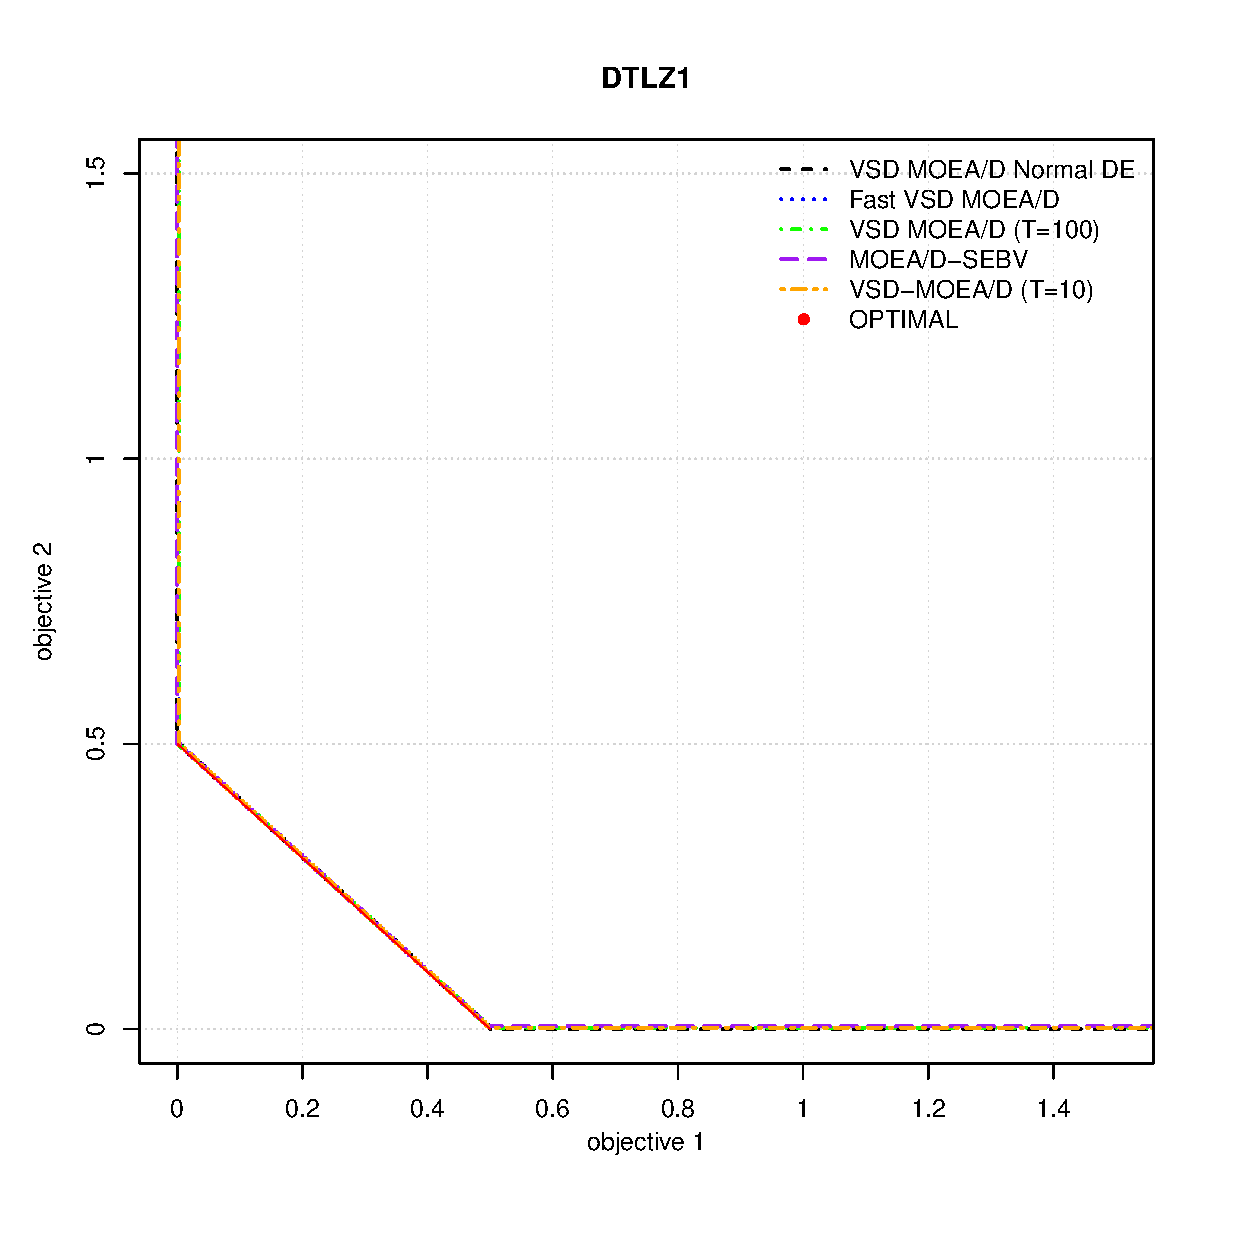
\includegraphics[scale=0.2]
{Figures_Chapter2/DTLZ1.jpg}
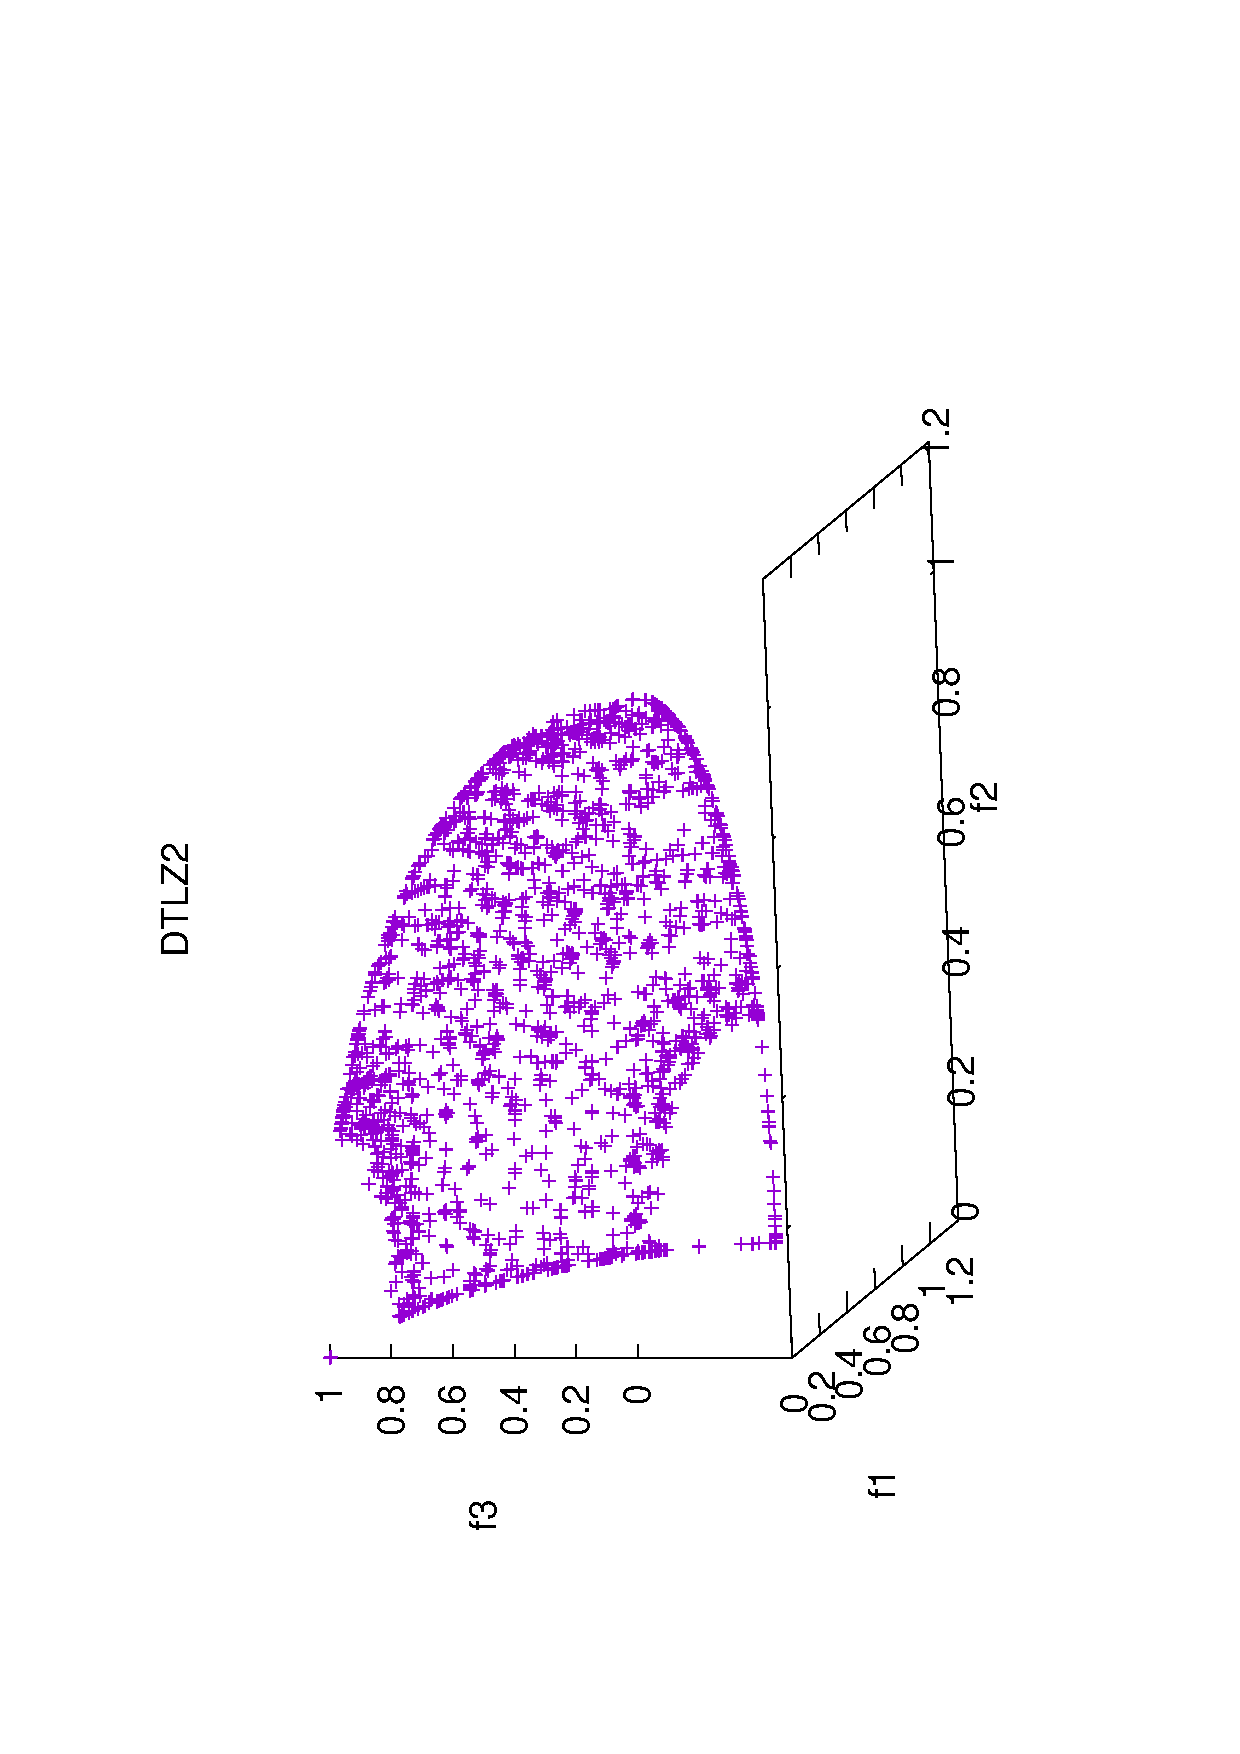
\includegraphics[scale=0.2]
{Figures_Chapter2/DTLZ2.jpg} \\
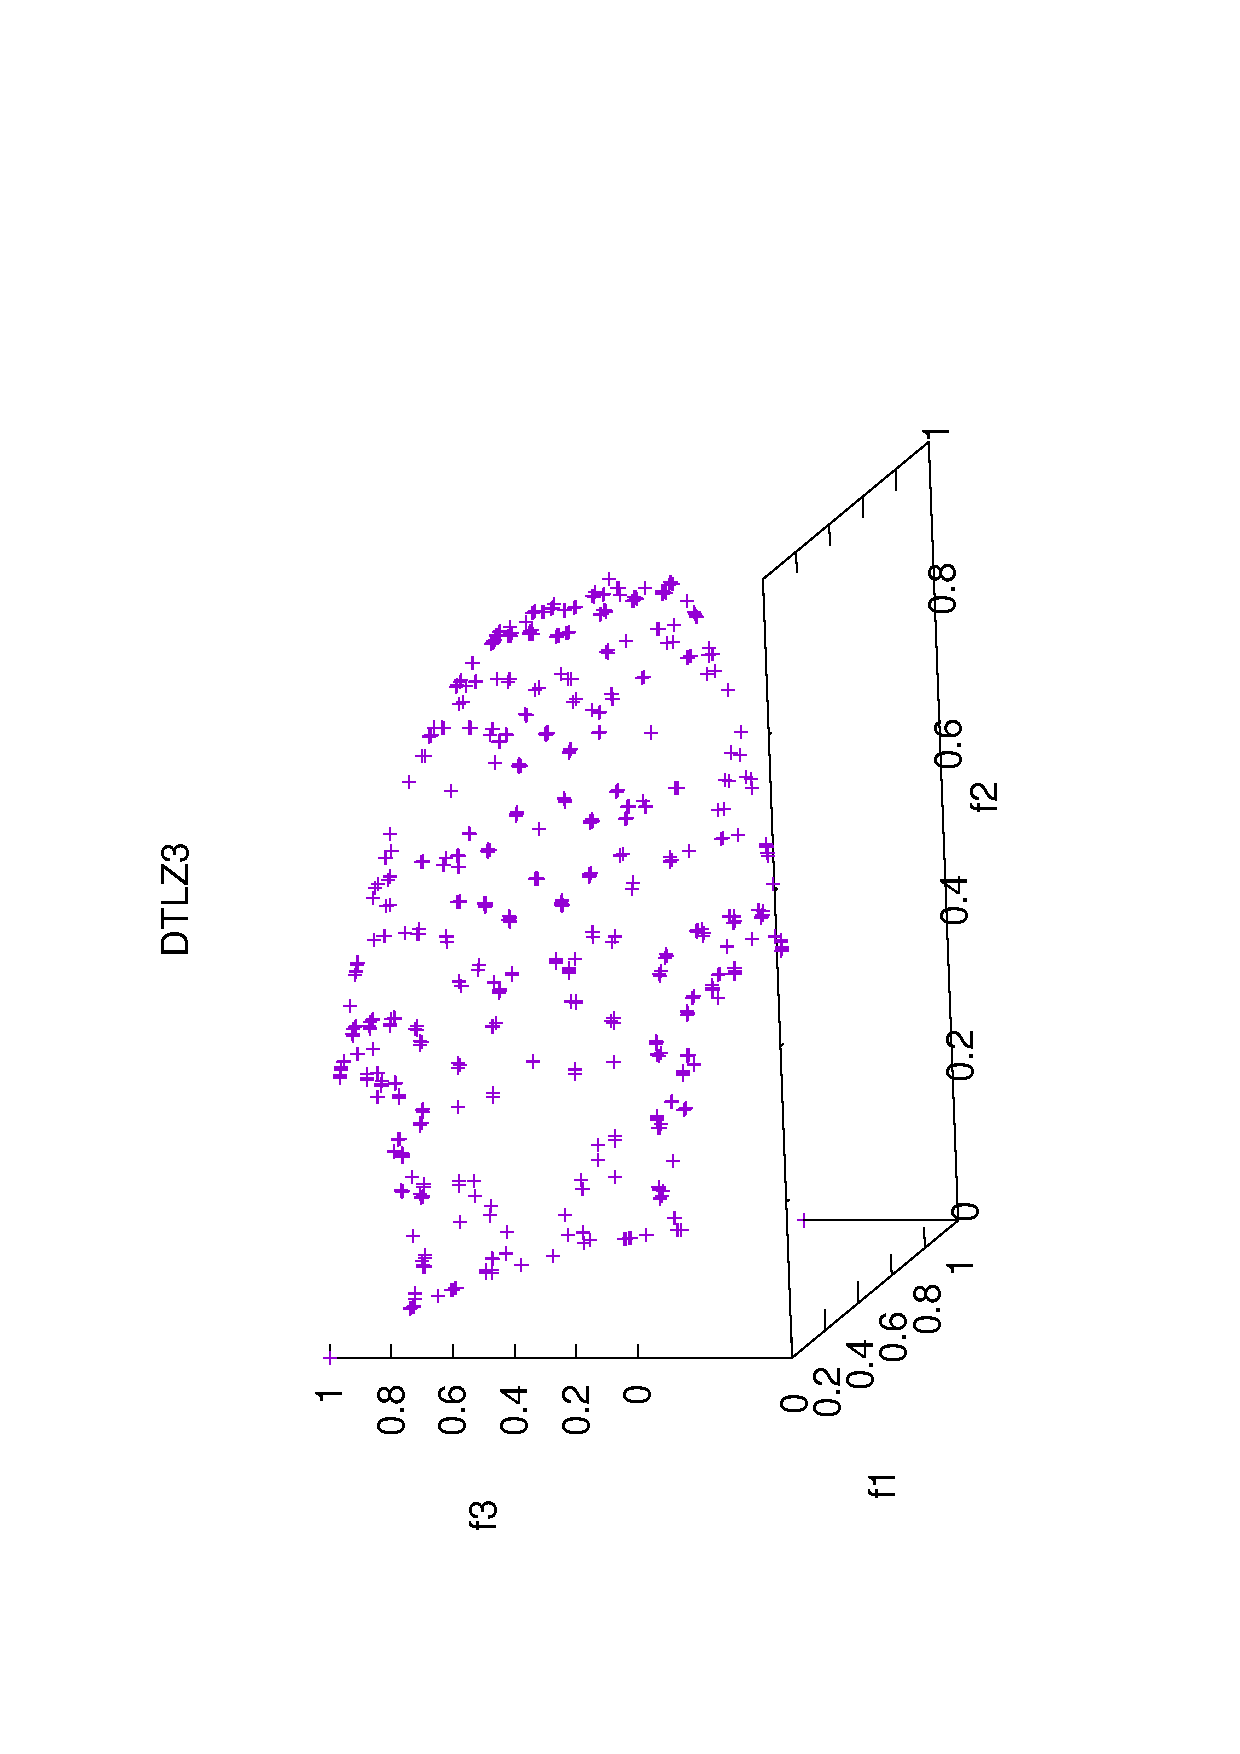
\includegraphics[scale=0.2]
{Figures_Chapter2/DTLZ3.jpg}
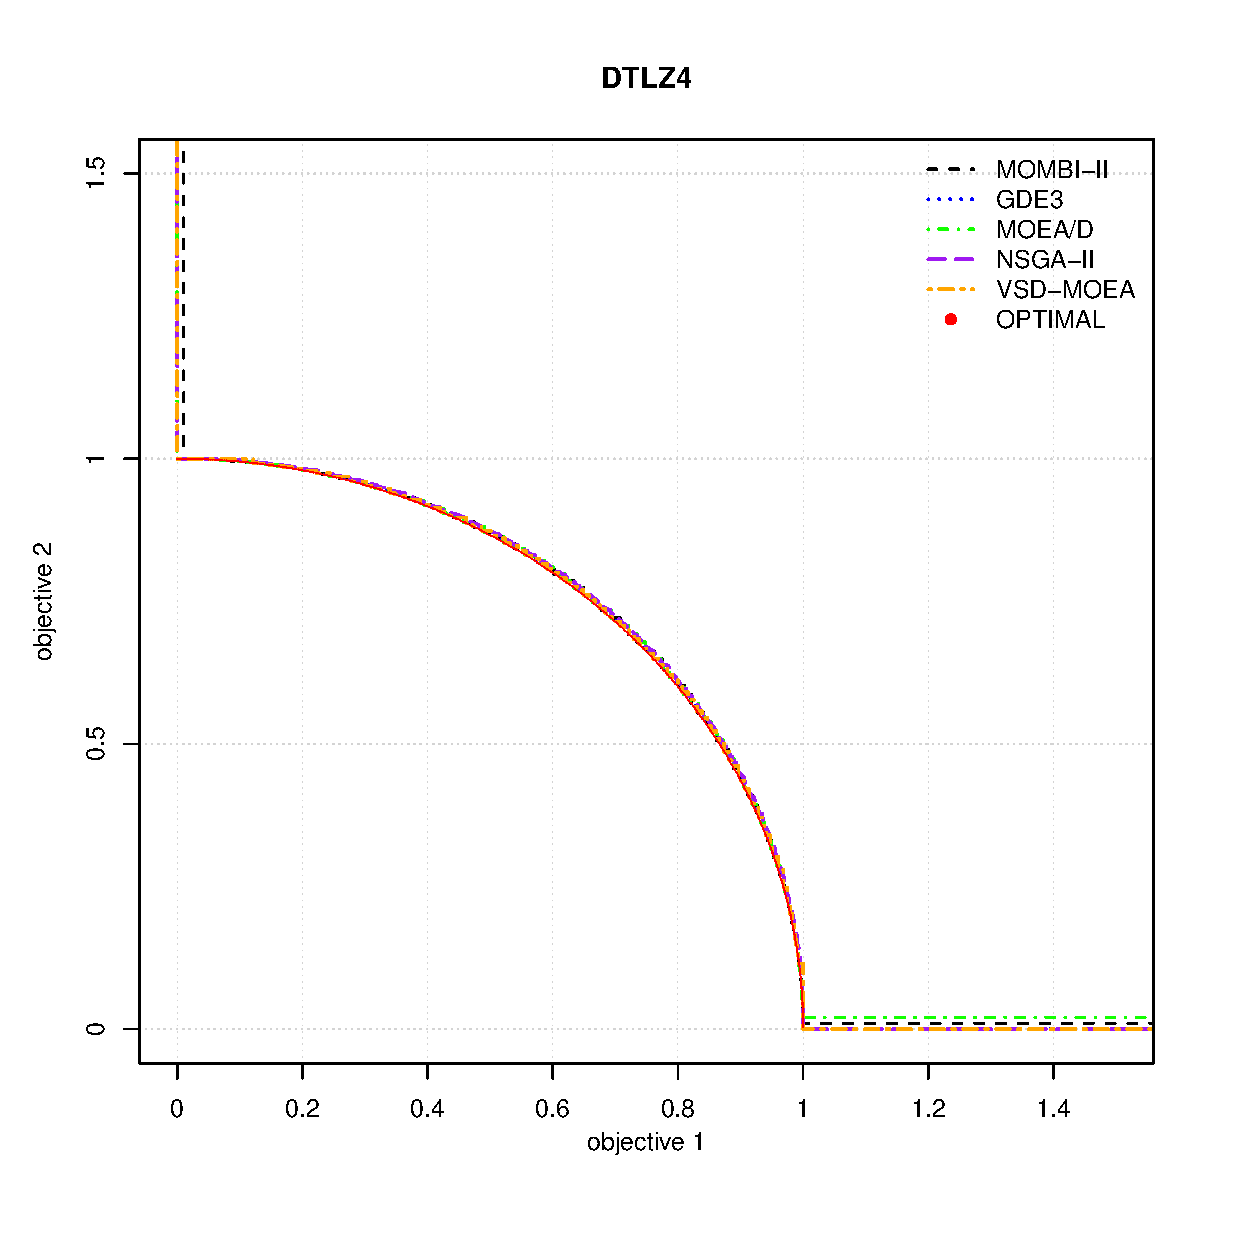
\includegraphics[scale=0.2]
{Figures_Chapter2/DTLZ4.jpg}\\
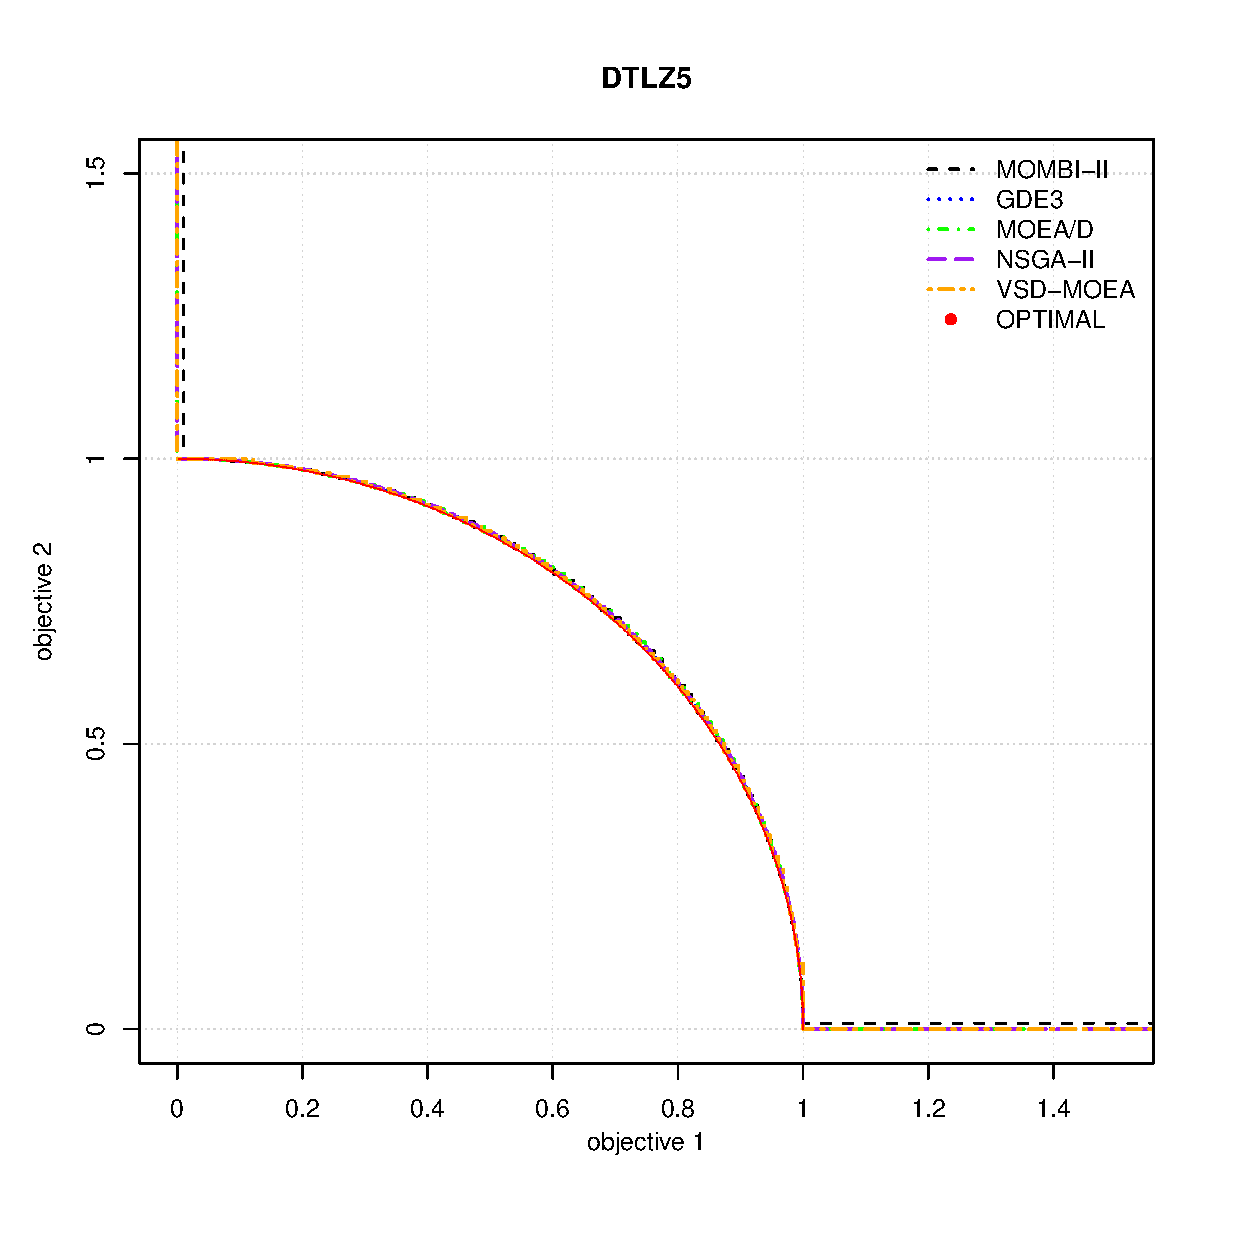
\includegraphics[scale=0.2]
{Figures_Chapter2/DTLZ5.jpg}
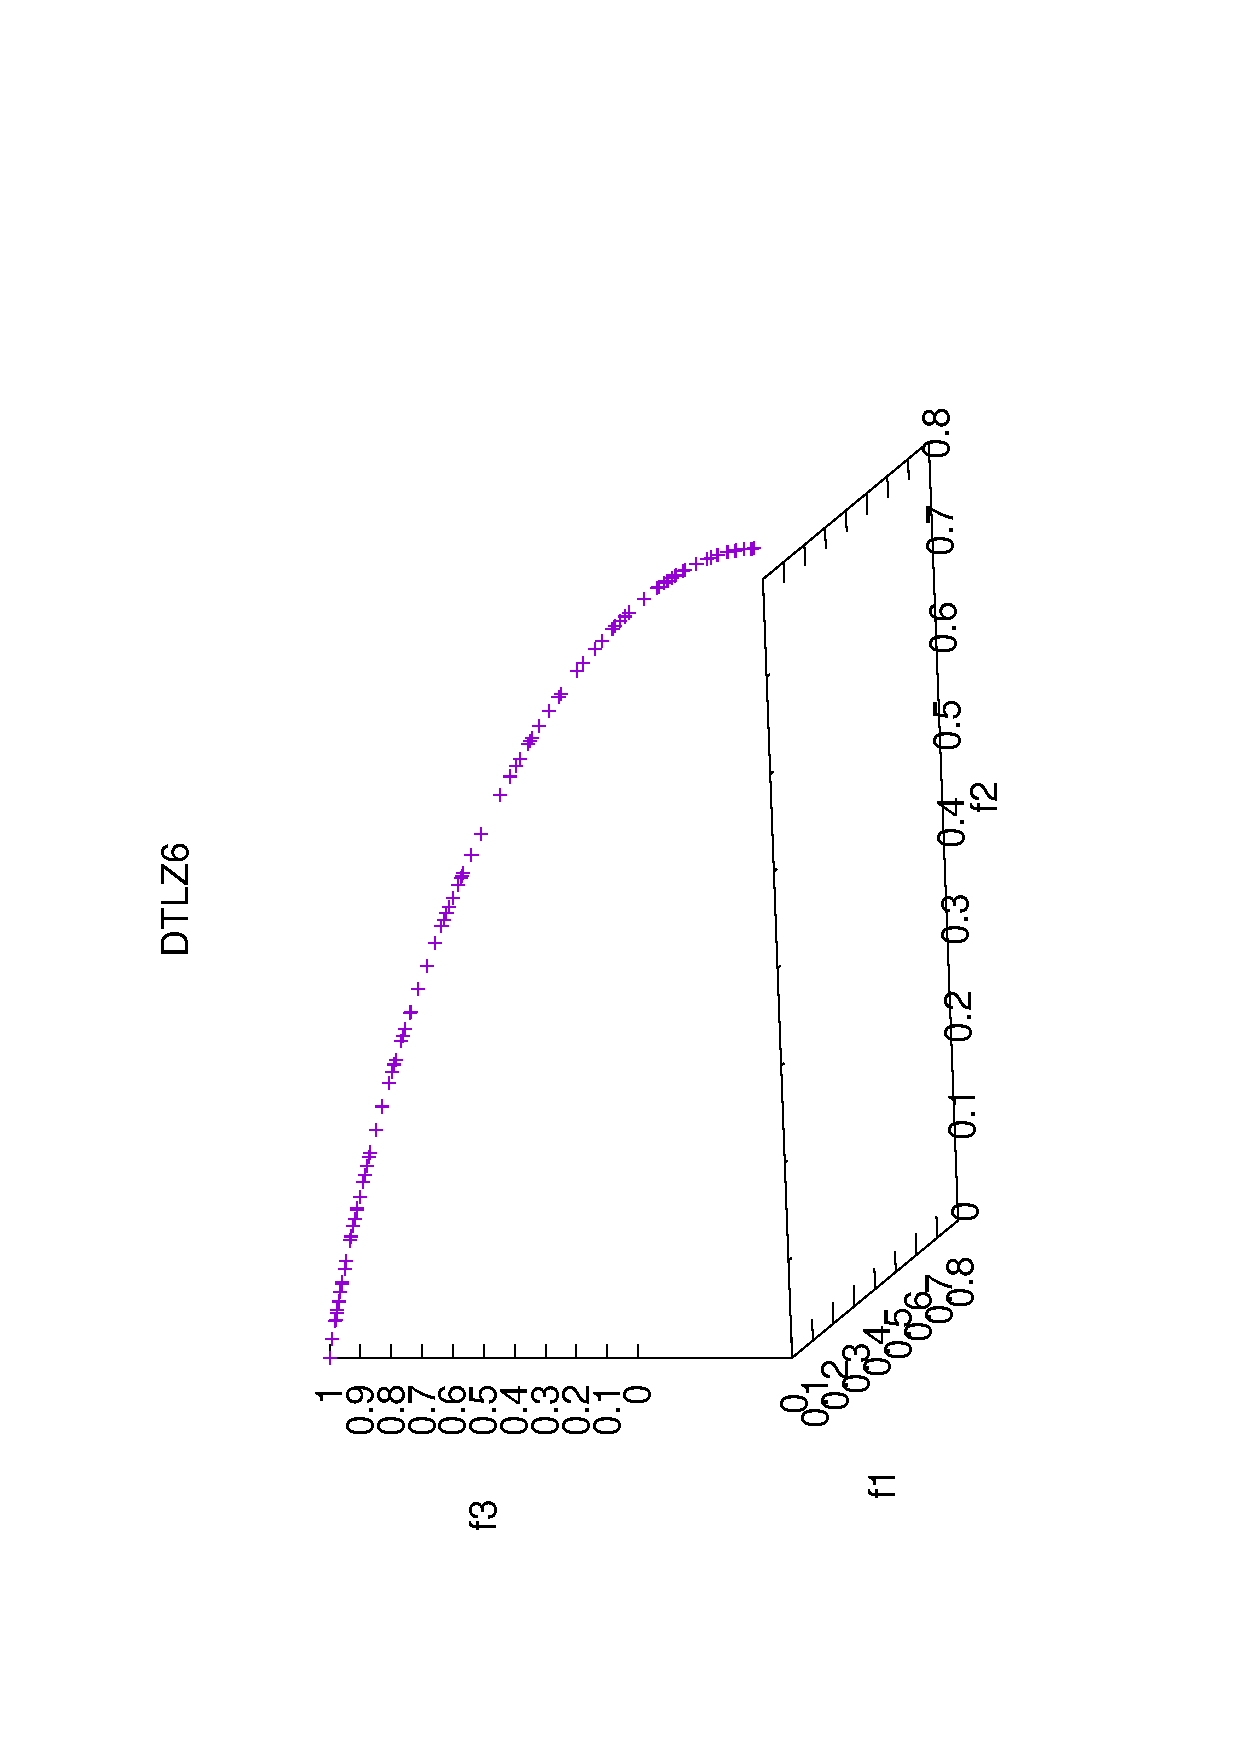
\includegraphics[scale=0.2]
{Figures_Chapter2/DTLZ6.jpg}\
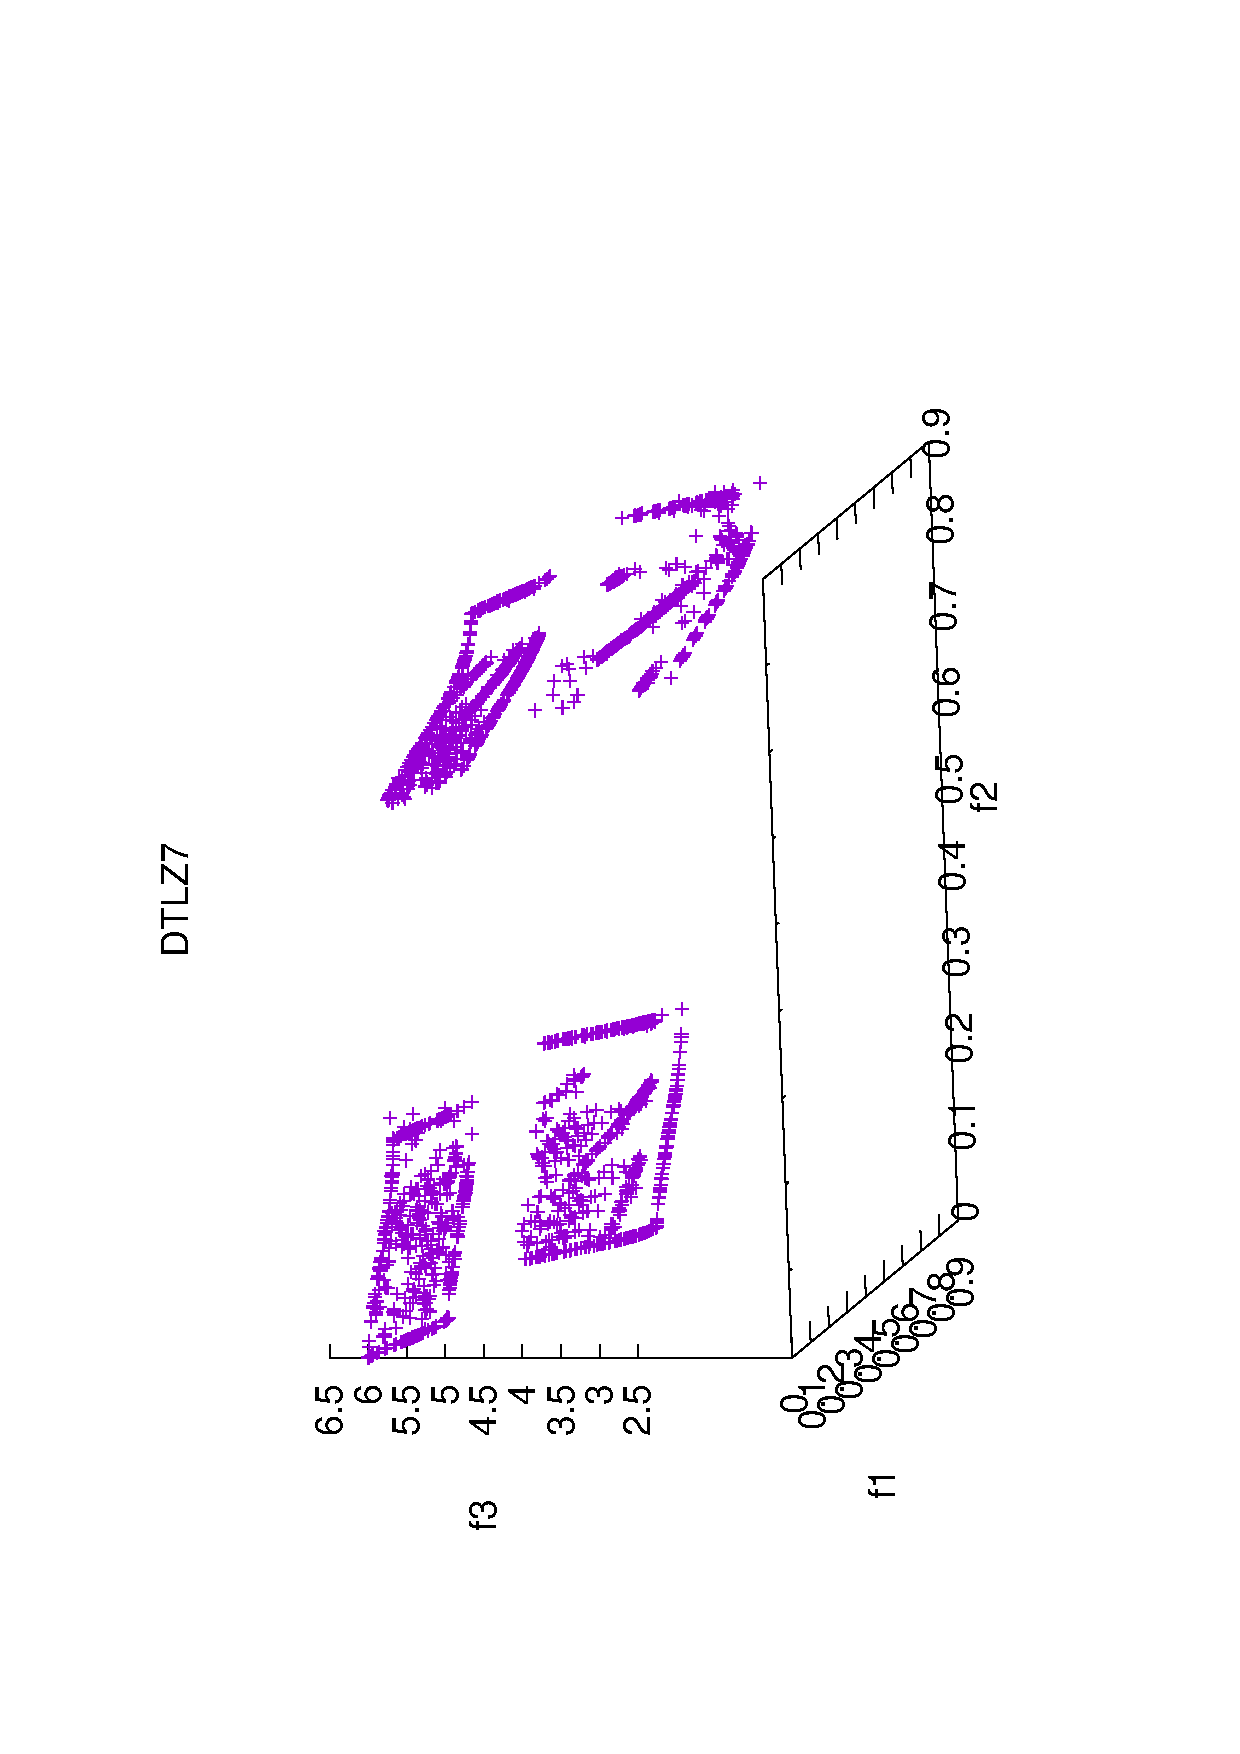
\includegraphics[scale=0.2]
{Figures_Chapter2/DTLZ7.jpg}
\end{figure}

% Please add the following required packages to your document preamble:
% \usepackage{graphicx}
\begin{table}[H]
\centering
\caption{Problemas DTLZ}
\label{tab:DTLZ}
\resizebox{\textwidth}{!}{%
\begin{tabular}{|c|l|c|}
\hline
Nombre & \multicolumn{1}{c|}{Problema} & Dominio de los parámetros \\ \hline
DTLZ1 & $ \begin{array}{lll}  f_1 &= (1+g) 0.5 \prod_{i=1}^{M-1} x_i \\ f_{m=2:M-1} &= (1+g) 0.5 (\prod_{i=1}^{M-m} x_i)(1 - y_{M-m+1}) \\ f_M &= (1+g) 0.5 (1-x_1) \\ g &= 100[x_M+\sum_{x_i \in x_M} (  (x_i - 0.5)^2 - cos(20 \pi (x_i - 0.5)) )] \end{array}$ & $[0,1]$ \\ \hline
DTLZ2 & $ \begin{array}{lll}   f_1 &= (1+g) \prod_{i=1}^{M-1} cos(x_i \pi/2) \\   f_{m=2:M-1} &= (1+g) \left (  \prod_{i=1}^{M-m} cos(x_i \pi / 2)   \right ) sin(x_{M-m+1} \pi / 2)   \\   f_M &= (1+g) sin(x_1 \pi /2) \\   g &= \sum_{x_i \in x_M} (x_i -0.5)^2 \end{array}$ & $[0,1]$ \\ \hline
DTLZ3 & Igual que DTLZ2, excepto que se utiliza la ecuación $g$ del DTLZ1 & $[0,1]$ \\ \hline
DTLZ4 & Igual que DTLZ2, excepto que $x_i \in x$ es reemplazado por $x_i ^ \alpha$, donde $\alpha > 0$ & $[0,1]$ \\ \hline
DTLZ5 & Igual que DTLZ2, excepto que $x_2, ..., x_{M-1} \in x $ son reemplazados por $\frac{1+2 g x_i}{2(1+g)}$ & $[0,1]$ \\ \hline
DTLZ6 & Igual que DTLZ5, excepto que la ecuación para $g$ es reemplazada por $g = \sum_{x_i \in x_M} x_i^{0.1}$ & $[0,1]$ \\ \hline
DTLZ7 & $ \begin{array}{lll} f_{m=1:M-1} &= x_m \\ f_M &= (1+g) \left (  M - \sum_{i=1}^{M-1} \left [ \frac{f_i}{1+g}(1 + sin(3 \pi f_i)) \right ] \right) \\ g &= 1+9 \sum_{x_i \in x_M} x_i /k \end{array}$ & $[0,1]$ \\ \hline
\end{tabular}%
}
\end{table}

\subsection{The Walking Fish Group (WFG)}
El toolkit WFG fue propuesto por \citeauthor{Joel:WFG_Main} en \citeyear{Joel:WFG_Main}, y provee las reglas para diseñar problemas personalizados, aunque en este trabajo se propusieron nueve instancias de ejemplo, éstas son utilizadas popularmente en el ámbito multi-objetivo.
%
Los problemas WFG dividen el espacio de las variables de decisión en dos subespacios: los parámetros de distancia y los parámetros de posición.
%
Un parámetro de distancia es aquel que al ser modificado siempre domina, es dominado o es un vector de parámetros equivalente.
%
Un parámetro de posición es aquel que cuando es modificado siempre resulta en un vector incomparable o un vector de parámetros equivalentes como se muestra en la figura \ref{fig:ParametrosWFG}.
%

Los nueve problemas de prueba propuestos emplean un número de funciones de transformación que facilitan la creación de vectores de transición, para dar al lector un panorama general se muestran las transiciones de cada problema de ejemplo en la tabla \ref{tab:WFG}, sin embargo no se presenta el gráfico de los frentes de Pareto debido a que sus respectivas formas están definidas por la configuración de los $l$ parámetros de distancia y los $k$ parámetros de posición, no obstante se pueden observar sus propiedades en la tabla \ref{tab:Propiedades}.
%
\subsubsection*{Observaciones WFG}
La instancia WFG1 distorsiona la importancia de cada parámetro por medio de distintos pesos mediante una reducción con suma de pesos, únicamente las instancias WFG1 y WFG7 son separables y unimodales, por otro lado la propiedad de no separabilidad de las instancias WFG6 y WFG9 provoca más dificultad en comparación a las instancias WFG2 y WFG3, la multimodalidad del WFG4 posee regiones óptimas más pronunciadas siendo más difícil que la multimodalidad de la instancia WFG9.
%
La deceptividad de la instancia WFG5 es más difícil que la instancia WFG9 ya que esta última sólo es deceptiva en los parámetros de posición.
%
Los parámetros de distancia de la instancia WFG8 son dependientes a los parámetros de posición (y entre los mismos parámetros de distancia) conformando un problema no separable.
%
Entonces en base a sus características, las instancias que se pueden considerar más difíciles son WFG5, WFG6, WFG8 y WFG9 a causa de su deceptividad, multimodalidad y dependencia.
%

Para las instancias WFG1-WFG7 una solución es óptimo de Pareto si todos los parámetros de distancia  $z_{i=k+1:n} = 2 i \times 0.35 $, particularmente el problems WFG2 es desconectado.
%
Para el problema WFG8 una solución es óptimo de Pareto si:
\begin{equation*}
\scriptsize
\begin{split}
z_{i=k+1:n} &= 2 i \times 0.35^{ \left  (   0.02 + 49.98  \left ( \frac{0.98}{49.98} - (1-2u) \left | \lfloor 0.5 - u \rfloor + \frac{0.98}{49.98} \right 	| \right  )            \right   )^{-1}    } \\
u &= r\_sum( \{ z_1, ..., z_{i-1} \}, \{ 1, ..., 1 \})
\end{split}
\end{equation*}  
Para el problema WFG9 una solución es óptimo de Pareto si:
\begin{equation*}
\scriptsize
\begin{split}
z_{i=k+1:n} &= 2 i  \begin{cases}\times 0.35^{  (0.02 + 1.96 u   )^{-1}    } & si \quad i \neq n \\ 0.35 & si \quad i=n \end{cases} \\
u &= r\_sum( \{ z_1, ..., z_{i-1} \}, \{ 1, ..., 1 \})
\end{split}
\end{equation*}

\begin{figure}[H]
\centering
\scriptsize
\includegraphics[scale=0.30]
{Figures_Chapter2/Parametros_Posicion_Distancia.png}
\caption{Par\'ametros de posici\'on y distancia de los problemas WFG}
\label{fig:ParametrosWFG}
\end{figure}



% Please add the following required packages to your document preamble:
% \usepackage{graphicx}
\begin{table}[]
\centering
\caption{Problemas de prueba WFG}
\label{tab:WFG}
\resizebox{\textwidth}{!}{%
\begin{tabular}{|l|l|c|}
\hline
\multicolumn{1}{|c|}{Nombre} & \multicolumn{1}{c|}{Problema} & Dominio de los parámetros \\ \hline
WFG1 & \begin{tabular}[c]{@{}l@{}}$\begin{array}{lll}      t^1_{i=1:k} &= x_i \\ t^1_{k+1:n} &= s\_linear(x_i, 0,35) \\ t^2_{i=1:k} &= x_i \\ t^2_{i=k+1:n} &= b\_flat(x_i, 0.8, 0.75, 0.85) \\ t^3_{i=1:n} &= b\_poly(x_i, 0.02) \\ t^4_{i=1:M-1} &= r\_sum(  \{ x_{(i-1)k/(M-1)+1},...,y_{ik/(M-1)} \}, \\  &\{ 2((i-1)k/(M-1)+1), ..., 2ik/(M-1) \} ) \\ t^4_M &= r\_sum( \{x_{k+1},...,y_n\}, \{ 2(k+1), ..., 2n \}) \\ h_{m=1:M-1} &= convex_m\\ \end{array}$\end{tabular} & $[0, 2 i]$ \\ \hline
WFG2 & \begin{tabular}[c]{@{}l@{}}Implementar $t^1$ del WFG1\\ $ \begin{array}{lll} t^2_{i=1:k}  &= x_i\\    t^2_{i =k+1:k+l/2} &= r\_nonsep(\{ x_{k+2(i-k)-1}, z_{k+2(i-k)}  \}, 2 )\\    t^3_{i=1:M-1} &= r\_sum( \{  x_{(i-1)k / (M-1) +1}, ..., x_{ik / (M-1)}  \}, \{1,...,1\} )\\    t^3_M &= r\_sum( \{ y_{k+1},..., y_{k+l/2}  \},\{1,...,1\} )\\    h_{m=1:M-1} &= convex_m\\    h_M &= disc_M ( \alpha = \beta =1, A = 5)\\  \end{array}$\end{tabular} & $[0, 2 i]$ \\ \hline
WFG3 & \begin{tabular}[c]{@{}l@{}}Implementar $t^1$, $t^2$ y $t^3$ del WFG2\\ $h_{m=1:M} = linear_m$\end{tabular} & $[0, 2 i]$ \\ \hline
WFG4 & \begin{tabular}[c]{@{}l@{}}$\begin{array}{lll}  t^1_{i=1:n} &= s\_multi(x_i, 30, 10, 0.35)\\   t^2_{i=1:M-1} &= r\_sum(\{ x_{(i-1)k / (M-1)+1},..., x_{ik / (M-1)}  \}, \{1,...,1\})\\   t^2_M &= r\_sum( \{ x_{k+1}, ..., x_n  \}, \{1,...,1\})\\   h_{m=1:M} &= concave_m\\ \end{array}$\end{tabular} & $[0, 2 i]$ \\ \hline
WFG5 & \begin{tabular}[c]{@{}l@{}}$t^1_{i=1:n} = s\_decept(x_i, 0.35, 0.001, 0.05)$\\ Implementar $t^2$ del WFG4 \\ $h_{m=1:M} = concave_m$\end{tabular} & $[0, 2 i]$ \\ \hline
WFG6 & \begin{tabular}[c]{@{}l@{}}Implementar $t^1$ del WFG1\\ $\begin{array}{lll} t^2_{i=1:M-1} &= r\_nonsep(\{y_{(i-1)k / (M-1) +1}, ..., y_{ik / (M-1)}\}, k/(M-1))\\  t^2_M &= r\_nonsep(\{ y_{k+1}, ..., y_n \}, l)\\ h_{m=1:M} &=concave_m\\  \end{array}$\end{tabular} & $[0, 2 i]$ \\ \hline
WFG7 & \begin{tabular}[c]{@{}l@{}}$\begin{array}{lll} t^1_{i=1:k} &= b\_param(x_i, r\_sum(\{ x_{i+1}, ..., x_n \},\{1,...,1\}), \frac{0.98}{49.88}, 0.02, 50)\\    t^1_{i=k+1:n} &=x_i\\    \end{array}$\\ Implementar $t^1$ del WFG1\\ Implementar $t^2$ del WFG4\\ $h_{m=1:M} = concave_m$\end{tabular} & $[0, 2 i]$ \\ \hline
WFG8 & \begin{tabular}[c]{@{}l@{}}$\begin{array}{lll}   t^1_{i=1:k} &= x_i\\    t^1_{k+1:n} &= b\_param( x_i, r\_sum( \{ x_1,, ...., x_{i-1} \}, \{ 1,..., 1\} ) , \frac{0.98}{49.98}, 0.02, 50)\\   \end{array}$\\ Implementar $t^2$ del WFG1\\ Implementar $t^2$ del WFG4\\ $h_{m=1:M} = concave_m$\end{tabular} & $[0, 2 i]$ \\ \hline
WFG9 & \begin{tabular}[c]{@{}l@{}}$\begin{array}{lll}t^1_{i=1:n-1} &= b\_param( x_i, r\_sum(  \{ y_{i+1}, ..., y_n \}, \{1,...,1\} ), \frac{0.98}{49.98}, 0.02, 50 )\\ t^1_{n} &= x_n\\ t^2_{i=1:k} &= s\_decept(x_i, 0.35, 0.001, 0.05)\\ t^2_{i=k+1:n} &= s\_multi(x_i, 30, 95, 0.35)\\ \end{array}$\\ Implementar $t^2$ del WFG6\\ $h_{m=1:M} = concave_m$\end{tabular} & $[0, 2 i]$ \\ \hline
\end{tabular}%
}
\end{table}

\subsection{Problemas de prueba sin restricciones (UF)}
Aunque los problemas ZDT, DTLZ y WFG, son muy implementados en el ámbito multi-objetivo, se ha propuesto un nuevo conjunto de problemas en el Congreso de Computo Evolutivo 2009 (Congress on Evolutionary Computation - CEC2009) por \cite{Joel:CEC2009}, denominados como UF (Unconstrained Functions) las cuales están compuestos por 10 problemas, donde los primeros 7 son específicamente para minimización dos objetivos y el resto de instancias son para minimización de tres objetivos. 
%

% Please add the following required packages to your document preamble:
% \usepackage{graphicx}
\begin{table}[]
\centering
\caption{Expresión del frente de Pareto y el conjunto de Pareto de los problemas UF}
\label{tab:Optimos_UF}
\resizebox{\textwidth}{!}{%
\begin{tabular}{|c|c|c|c|}
\hline
Nombre & Frente de Pareto & Conjunto de Pareto & Variables Recomendadas \\ \hline
UF1 & \begin{tabular}[c]{@{}c@{}}$f_2= 1 - \sqrt{f_1}$\\  $0 \leq f_1 \leq 1$\end{tabular} & \begin{tabular}[c]{@{}c@{}}$x_j = sin(6 \pi x_1 + \frac{j \pi}{n})$\\  $ j=2,...,n $\\ $0 \leq x_1 \leq 1$\end{tabular} & 30 \\ \hline
UF2 & \begin{tabular}[c]{@{}c@{}}$f_2= 1 - \sqrt{f_1}$\\  $0 \leq f_1 \leq 1$\end{tabular} & $ x_j =\begin{cases} \{ 0.3x_1^2 cos(24 \pi x_1 + \frac{4 j \pi}{n}) + 0.6 x_1 \} \times \\cos( 6 \pi x_1 + \frac{j \pi}{n}) \\ j \in J_1 \\ \{ 0.3x_1^2 cos(24 \pi x_1 + \frac{4 j \pi}{n}) + 0.6 x_1 \}\times \\ cos( 6 \pi x_1 + \frac{j \pi}{n}) \\ j \in J_2,\end{cases} $ & 30 \\ \hline
UF3 & \begin{tabular}[c]{@{}c@{}}$f_2 = 1 - \sqrt{f_1}$\\  $0 \leq f_1 \leq 1$\end{tabular} & \begin{tabular}[c]{@{}c@{}}$x_j = x_1^{ 0.5(1.0 + \frac{3(j-2)}{n-2}) }$\\   $j=2, ..., n, \quad 0 \leq x_1 \leq 1$\end{tabular} & 30 \\ \hline
UF4 & \begin{tabular}[c]{@{}c@{}}$f_2= 1 - f_1^2$\\  $0 \leq f_1 \leq 1$\end{tabular} & \begin{tabular}[c]{@{}c@{}}$x_j = sin(6 \pi x_1 + \frac{j \pi}{n})$\\  $j=2,...,n, \quad 0 \leq x_1 \leq 1$\end{tabular} & 30 \\ \hline
UF5 & \begin{tabular}[c]{@{}c@{}}$(\frac{i}{2N}, 1 - \frac{i}{2N}) \quad \forall i = 0,1,..., 2N$\\ \\ $N=10$, $\epsilon = 0.1$ y $n = 30$.\end{tabular} &  & 30 \\ \hline
UF6 & \begin{tabular}[c]{@{}c@{}}Consiste de un punto aislado en (0,1) y $N$ partes desconectadas\\ $f_2= 1 - f_1, f_1 \in \bigcup\limits_{i=1}^{N} [ \frac{2i - 1}{2N}$\\ $\frac{2i}{2N}]$\end{tabular} &  & 30 \\ \hline
UF7 & \begin{tabular}[c]{@{}c@{}}$f_2= 1 - f_1$\\  $0 \leq f_1 \leq 1$\end{tabular} & \begin{tabular}[c]{@{}c@{}}$x_j = sin(6 \pi x_1 + \frac{j \pi}{n})$\\ $j=2,...,n$\\ $0 \leq x_1 \leq 1$\end{tabular} & 30 \\ \hline
UF8 & \begin{tabular}[c]{@{}c@{}}$f_1^2 + f_2^2 + f_3^2 = 1$\\ $0 \leq f_1, f_2, f_3 \leq 1$\end{tabular} & \begin{tabular}[c]{@{}c@{}}$x_j = 2 x_2 sin(2 \pi x_1 + \frac{j \pi}{n})$\\ $j=3,...,n $\end{tabular} & 30 \\ \hline
UF9 & \begin{tabular}[c]{@{}c@{}}La primer parte es \\ $0 \leq f_3 \leq 1$\\ \\  $0 \leq f_1 \leq \frac{1}{4} (1 - f_3)$\\ \\ $f_2 = 1 - f_1 - f_3$\\ \\ La segunda parte es \\ $0 \leq f_3 \leq 1$, \\ \\ $\frac{3}{4} (1 - f_3) \leq f_1 \leq 1,$\\ \\ $f_2 = 1 - f_1 - f_3$\end{tabular} & \begin{tabular}[c]{@{}c@{}}Tiene dos partes desconectadas\\ $x_1 \in [0, 0.25] \cup [0.75, 1] \quad 0 \leq x_2 \leq 1$\\ \\ $x_j = 2 x_2 sin(2 \pi x_1 + \frac{j \pi}{n}), \quad j=3,...,n$\end{tabular} & 30 \\ \hline
UF10 & \begin{tabular}[c]{@{}c@{}}$f_1^2 + f_2^2 + f_3^2 = 1$ \\ $ 0 \leq f_1, f_2, f_3 \leq 1$\end{tabular} & $x_j = 2 x_2 sin (2 \pi x_1 + \frac{j \pi}{n}), \quad j=3,...,n$ & 30 \\ \hline
\end{tabular}%
}
\end{table}


%\subsubsection*{Función de prueba UF1}
%\begin{equation*}
%\scriptsize
%\begin{split}
%& minimizar \quad f_1= x_1 + \frac{2}{|J_1|} \sum_{j \in J_1} [x_j - sin(6 \pi x_1 + \frac{j \pi}{n})]^2 \\
%& minimizar \quad f_2 = 1 - \sqrt{x_1} + \frac{1}{|J_2|} \sum_{j \in J_2} [x_j - sin( 6 \pi x_1 + \frac{j \pi}{n}]^2
%\end{split}
%\end{equation*}
% Donde
% $J_1 = \{ j|j$ es impar y $2 \leq j \leq n \}$ y $J_2 = \{ j|j$ es par con $2 \leq j \leq n \}$, el espacio de búsqueda esta comprendido por $[0, 1] \times [-1,1]^{n-1}$.
 %
 
% El frente de Pareo óptimo es:
% \begin{equation*}
% f_2= 1 - \sqrt{f_1}, \quad 0 \leq f_1 \leq 1
% \end{equation*}
% %
% 
% El conjunto de Pareto está definido por:
% \begin{equation*}
%x_j = sin(6 \pi x_1 + \frac{j \pi}{n}), \quad j=2,...,n, \quad 0 \leq x_1 \leq 1
% \end{equation*}
%
%El número de variables utilizadas son $n=30$.
%\begin{figure}[H]
%\centering
%\scriptsize
%\includegraphics[scale=0.5]
%{Figures_Chapter2/UF1.eps}
%%\decoRule
%\caption{Frente de Pareto y conjunto de Pareto del problema UF1}
%\label{fig:UF1}
%\end{figure}

%\subsubsection*{Función de prueba UF2}
%\begin{equation*}
%\scriptsize
%\begin{split}
%& minimizar \quad f_1= x_1 + \frac{2}{|J_1|} \sum_{j \in J_1} y_j^2 \\
%& minimizar \quad f_2 = 1 - \sqrt{x_1} + \frac{1}{|J_2|} \sum_{j \in J_2} y_j^2
%\end{split}
%\end{equation*}
% Donde
% $J_1 = \{ j|j$ es impar y $2 \leq j \leq n \}$ y $J_2 = \{ j|j$ es par con $2 \leq j \leq n \}$, el espacio de búsqueda esta comprendido por $[0, 1] \times [-1,1]^{n-1}$.
% %
% \begin{equation}
% y_j = 
% \begin{cases}
% x_j - [0.3x_1^2 cos(24 \pi x_1 + \frac{4 j \pi}{n}) + 0.6 x_1] cos( 6 \pi x_1 + \frac{j \pi}{n} \quad j \in J_1 \\
% x_j - [0.3x_1^2 cos(24 \pi x_1 + \frac{4 j \pi}{n}) + 0.6 x_1] cos( 6 \pi x_1 + \frac{j \pi}{n} \quad j \in J_2 
% \end{cases}
% \end{equation}
 %
% El frente de Pareo óptimo es:
% \begin{equation*}
% f_2= 1 - \sqrt{f_1}, \quad 0 \leq f_1 \leq 1
% \end{equation*}
% %
% 
% 
% El conjunto de Pareto es:
% \begin{equation*}
% x_j = 
% \begin{cases}
% \{ 0.3x_1^2 cos(24 \pi x_1 + \frac{4 j \pi}{n}) + 0.6 x_1 \} cos( 6 \pi x_1 + \frac{j \pi}{n} \quad j \in J_1 \\
% \{ 0.3x_1^2 cos(24 \pi x_1 + \frac{4 j \pi}{n}) + 0.6 x_1 \} cos( 6 \pi x_1 + \frac{j \pi}{n} \quad j \in J_2 
% \end{cases}
% \end{equation*}
%El número de variables utilizadas son $n=30$.
%\begin{figure}[H]
%\centering
%\scriptsize
%\includegraphics[scale=0.5]
%{Figures_Chapter2/UF2.eps}
%\caption{Frente de Pareto y conjunto de Pareto del problema UF2}
%\label{fig:UF2}
%\end{figure}


%\subsubsection*{Función de prueba UF3}
%\begin{equation*}
%\scriptsize
%\begin{split}
%& minimizar \quad f_1= x_1 + \frac{2}{|J_1|} ( 4 \sum_{j \in J_1} y_j^2 - 2 \prod_{j \in J_1} cos (  \frac{20 y_j \pi}{ \sqrt[]{j}} ) + 2 ) \\
%& minimizar \quad f_2=  1 - \sqrt[]{x_1} + \frac{2}{|J_2|} ( 4 \sum_{j \in J_2} y_j^2 - 2 \prod_{j \in J_2} cos (  \frac{20 y_j \pi}{ \sqrt[]{j}} ) + 2 ) 
%\end{split}
%\end{equation*}
% Donde
% $J_1$ y $J_2$ son iguales como en F1, el espacio de búsqueda esta comprendido por $[0, 1]^n$.
% %
% \begin{equation*}
%    y_j = x_1^{ 0.5(1.0 + \frac{3(j-2)}{n-2}) }, \quad j=2, ..., n,
%\end{equation*}
 
% El frente de Pareo óptimo es:
% \begin{equation*}
%   f_2 = 1 - \sqrt[]{f_1}, \quad 0 \leq f_1 \leq 1.
%\end{equation*}
%
% %
% El conjunto de Pareto es:
% \begin{equation*}
%	x_j = x_1^{ 0.5(1.0 + \frac{3(j-2)}{n-2}) }, \quad j=2, ..., n, \quad 0 \leq x_1 \leq 1. 
% \end{equation*}
%
%El número de variables utilizadas son $n=30$
%\begin{figure}[H]
%\centering
%\scriptsize
%\includegraphics[scale=0.5]
%{Figures_Chapter2/UF3.eps}
%\caption{Frente de Pareto y conjunto de Pareto del problema UF3}
%\label{fig:UF3}
%\end{figure}


%\subsubsection*{Función de prueba UF4}
%\begin{equation*}
%\scriptsize
%\begin{split}
%& minimizar \quad f_1= x_1 + \frac{2}{|J_1|} \sum_{j \in J_1} h(y_j)\\
%& minimizar \quad f_2= 1 - x_1^2 + \frac{2}{|J_2|} \sum_{j \in J_2} h(y_j)
%\end{split}
%\end{equation*}
% Donde
% $J_1 = \{ j|j$ es impar y $2 \leq j \leq n \}$ y $J_2 = \{ j|j$ es par con $2 \leq j \leq n \}$, el espacio de búsqueda esta comprendido por $[0, 1] \times [-2,2]^{n-1}$.
% %
% \begin{equation*}
% \begin{split}
% y_j = x_j - sin( 6 \pi x_1 + \frac{j \pi}{ n} ), j=2, ..., n. \\
% h(t) = \frac{|t|}{ 1 ++ e^{2 |t| }}
% \end{split}
% \end{equation*}
 
% El frente de Pareo óptimo es:
% \begin{equation*}
% f_2= 1 - f_1^2, \quad 0 \leq f_1 \leq 1
% \end{equation*}
%
% %
% El conjunto de Pareto es:
% \begin{equation*}
%x_j = sin(6 \pi x_1 + \frac{j \pi}{n}), \quad j=2,...,n, \quad 0 \leq x_1 \leq 1
% \end{equation*}
%
%El número de variables utilizadas son $n=30$

%\begin{figure}[H]
%\centering
%\scriptsize
%\includegraphics[scale=0.5]
%{Figures_Chapter2/UF4.eps}
%\caption{Frente de Pareto y conjunto de Pareto del problema UF4}
%\label{fig:UF4}
%\end{figure}

%\subsubsection*{Función de prueba UF5}
%\begin{equation*}
%\scriptsize
%\begin{split}
%& minimizar \quad f_1= x_1 +  (\frac{1}{2N} + \epsilon) | sin(2 N \pi x_1)  +\frac{2}{|J_1|} \sum_{j \in J_1} h(y_j)\\
%& minimizar \quad f_2= 1 - x_1 +  (\frac{1}{2N} + \epsilon) | sin(2 N \pi x_1)  +\frac{2}{|J_2|} \sum_{j \in J_2} h(y_j)\\
%\end{split}
%\end{equation*}
% Donde
% $J_1 = \{ j|j$ es impar y $2 \leq j \leq n \}$ y $J_2 = \{ j|j$ es par con $2 \leq j \leq n \}$. N es un entero, $\epsilon >0$ ,el espacio de búsqueda esta comprendido por $[0, 1] \times [-1,1]^{n-1}$.
% %
% \begin{equation*}
% \begin{split}
% y_j = x_j - sin( 6 \pi x_1 + \frac{j \pi}{ n} ), j=2, ..., n. \\
% h(t) = 2t^2 - cos(4 \pi t) + 1
% \end{split}
% \end{equation*}
 
% El frente de Pareo óptimo tiene 2N + 1 soluciones:
% \begin{equation*}
%(\frac{i}{2N}, 1 - \frac{i}{2N}) \quad \forall i = 0,1,..., 2N.
% \end{equation*}
%$N=10$, $\epsilon = 0.1$ y $n = 30$.

%\begin{figure}[H]
%\centering
%\scriptsize
%\includegraphics[scale=0.5]
%{Figures_Chapter2/UF5.eps}
%\caption{Frente de Pareto y conjunto de Pareto del problema UF5}
%\label{fig:UF5}
%\end{figure}

%\subsubsection*{Función de prueba UF6}
%\begin{equation*}
%\scriptsize
%\begin{split}
%& minimizar \quad f_1= x_1 + max \{ 0,  2(\frac{1}{2N} + \epsilon ) sin(2N \pi x_1)  \} + \frac{2}{|J_1|} ( 4 \sum_{j \in J_1} y_j^2 - 2 \prod_{j \in J_1} cos( \frac{20 y_j \pi}{\sqrt[]{j}} ) + 2  )  \\
%& minimizar \quad f_2= 1 - x_1 + max \{ 0,  2(\frac{1}{2N} + \epsilon ) sin(2N \pi x_1)  \} + \frac{2}{|J_2|} ( 4 \sum_{j \in J_2} y_j^2 - 2 \prod_{j \in J_2} cos( \frac{20 y_j \pi}{\sqrt[]{j}} ) + 2  )  \\
%\end{split}
%\end{equation*}
% Donde
% $J_1 = \{ j|j$ es impar y $2 \leq j \leq n \}$ y $J_2 = \{ j|j$ es par con $2 \leq j \leq n \}$, el espacio de búsqueda esta comprendido por $[0, 1] \times [-1,1]^{n-1}$.
% %
% \begin{equation*}
% y_j= x_j - sin(6 \pi x_1 + \frac{j \pi}{n}), j=2,...,n.
% \end{equation*}
 
% El frente de Pareo óptimo consiste de un punto aislado y $N$ parte desconectadas.
% \begin{equation*}
% f_2= 1 - f_1, f_1 \in \bigcup\limits_{i=1}^{N} [ \frac{2i - 1}{2N}, \frac{2i}{2N}].
% \end{equation*}
%$N=2$, $\epsilon = 0.1$ y $n=30$.
% \begin{figure}[H]
%\centering
%\scriptsize
%\includegraphics[scale=0.5]
%{Figures_Chapter2/UF6.eps}
%\caption{Frente de Pareto y conjunto de Pareto del problema UF6}
%\label{fig:UF6}
%\end{figure}

%\subsubsection*{Función de prueba UF7}
%\begin{equation*}
%\scriptsize
%\begin{split}
%& minimizar \quad f_1= \sqrt[5]{x_1} + \frac{2}{|J_1|} \sum_{j \in J_1} y_j^2 \\
%& minimizar \quad f_2= 1 - \sqrt[5]{x_1} + \frac{2}{|J_2|} \sum_{j \in J_2} y_j^2 \\
%\end{split}
%\end{equation*}
% Donde
% $J_1 = \{ j|j$ es impar y $2 \leq j \leq n \}$ y $J_2 = \{ j|j$ es par con $2 \leq j \leq n \}$, el espacio de búsqueda esta comprendido por $[0, 1] \times [-1,1]^{n-1}$.
% %
% \begin{equation*}
% y_j = x_j - sin(6 \pi x_1 + \frac{j \pi}{n} ), j=2,..., n
% \end{equation*}
 
% El frente de Pareo óptimo es
% \begin{equation*}
% f_2= 1 - f_1, \quad 0 \leq f_1 \leq 1
% \end{equation*}
%
% %
% El conjunto de Pareto es
% \begin{equation*}
%x_j = sin(6 \pi x_1 + \frac{j \pi}{n}), \quad j=2,...,n, \quad 0 \leq x_1 \leq 1
% \end{equation*}
%
%El número de variables utilizados son $n=30$
%\begin{figure}[H]
%\centering
%\scriptsize
%\includegraphics[scale=0.5]
%{Figures_Chapter2/UF7.eps}
%\caption{Frente de Pareto y conjunto de Pareto del problema UF7}
%\label{fig:UF7}
%\end{figure}

%\subsubsection*{Función de prueba UF8}
%\begin{equation*}
%\scriptsize
%\begin{split}
%& minimizar \quad f_1= cos(0.5 x_1 \pi) cos(0.5 x_2 \pi ) + \frac{2}{J_1} \sum_{j \in J_1} (x_j - 2 x_2 sin(2\pi x_1 + \frac{j \pi}{n}))^2\\
%& minimizar \quad f_2= cos(0.5 x_1 \pi) sin(0.5 x_2 \pi ) + \frac{2}{J_2} \sum_{j \in J_1} (x_j - 2 x_2 sin(2\pi x_1 + \frac{j \pi}{n}))^2\\
%& minimizar \quad f_3= sin(0.5 x_1 \pi ) + \frac{2}{J_3} \sum_{j \in J_1} (x_j - 2 x_2 sin(2\pi x_1 + \frac{j \pi}{n}))^2
%\end{split}
%\end{equation*}
% Donde
% $J_1 = \{ j|3 \leq j \leq n \}$, y $j-1$ es una multiplicación de 3, \\
% $J_2 = \{ j|3 \leq j \leq n \}$, y $j-2$ es una multiplicación de 3, \\
% $J_3 = \{ j|3 \leq j \leq n \}$, y $j$ es una multiplicación de 3. 
% %
%El espacio de búsqueda es $[0,1]^2 \times [-2, 2]^{n-2}$

% El frente de Pareo óptimo es
% \begin{equation*}
% f_1^2 + f_2^2 + f_3^2 = 1, 0 \leq f_1, f_2, f_3 \leq 1. 
% \end{equation*}
% %
% El conjunto de Pareto es
% \begin{equation*}
%x_j = 2 x_2 sin(2 \pi x_1 + \frac{j \pi}{n}), \quad j=3,...,n.
% \end{equation*}
%
%El número de variables utilizados son $n=30$
%\begin{figure}[H]
%\centering
%\scriptsize
%\includegraphics[scale=0.5]
%{Figures_Chapter2/UF8.eps}
%\caption{Frente de Pareto y conjunto de Pareto del problema UF8}
%\label{fig:UF8}
%\end{figure}

%\subsubsection*{Función de prueba UF9}
%\begin{equation*}
%\scriptsize
%\begin{split}
%& minimizar \quad f_1= 0.5[ max\{ 0,  (1 + \epsilon) (1 - 4(2 x_1 - 1)^2 ) \} + 2 x_1] x_2 + \frac{2}{|J_1|} \sum_{j \in J_1} ( x_j - 2 x_2 sin(2 \pi x_1 + \frac{j \pi}{n}) )^2\\
%& minimizar \quad f_2= 0.5[ max\{ 0,  (1 + \epsilon) (1 - 4(2 x_1 - 1)^2 ) \} - 2 x_1 + 2] x_2 + \frac{2}{|J_2|} \sum_{j \in J_2} ( x_j - 2 x_2 sin(2 \pi x_1 + \frac{j \pi}{n}) )^2\\
%& minimizar \quad f_3= 1 - x_2 + \frac{2}{|J_3|} \sum_{j \in J_3} ( x_j - 2 x_2 sin(2 \pi x_1 + \frac{j \pi}{n}) )^2
%\end{split}
%\end{equation*}
% Donde
% $J_1 = \{ j|3 \leq j \leq n \}$, y $j-1$ es una multiplicación de 3, \\
% $J_2 = \{ j|3 \leq j \leq n \}$, y $j-2$ es una multiplicación de 3, \\
% $J_3 = \{ j|3 \leq j \leq n \}$, y $j$ es una multiplicación de 3. \\
% $\epsilon = 0.1$\\
% %
%El espacio de búsqueda es $[0,1]^2 \times [-2, 2]^{n-2}$

% El frente de Pareo óptimo tiene dos partes. La primer parte es
%\begin{equation*}
%\begin{split}
%0 \leq f_3 \leq 1, \\
%0 \leq f_1 \leq \frac{1}{4} (1 - f_3),\\
%f_2 = 1 - f_1 - f_3
%\end{split}
%\end{equation*}
% %
%La segunda parte es:
%\begin{equation*}
%\begin{split}
%0 \leq f_3 \leq 1, \\
%\frac{3}{4} (1 - f_3) \leq f_1 \leq 1,\\
%f_2 = 1 - f_1 - f_3
%\end{split}
% \end{equation*}
% 
% %
%El conjunto de Pareto, también tiene dos partes:
% \begin{equation*}
% \begin{split}
%   x_1 \in [0, 0.25] \cup [0.75, 1], \quad 0 \leq x_2 \leq 1,\\
%   x_j = 2 x_2 sin (2 \pi x_1 + \frac{j \pi}{n}), \quad j=3,...,n.
% \end{split}
% \end{equation*}
%
%El número de variables utilizados son $n=30$

%\begin{figure}[H]
%\centering
%\scriptsize
%\includegraphics[scale=0.5]
%{Figures_Chapter2/UF9.eps}
%\caption{Frente de Pareto y conjunto de Pareto del problema UF9}
%\label{fig:UF9}
%\end{figure}
%\subsubsection*{Función de prueba UF10}
%\begin{equation*}
%\scriptsize
%\begin{split}
%& minimizar \quad f_1= cos(0.5 x_1 \pi ) cos(0.5 x_2 \pi) + \frac{2}{|J_1|} \sum_{j \in J_1} [ 4 y_j^2 - cos( 8 \pi y_j) + 1] \\
%& minimizar \quad f_2= cos(0.5 x_1 \pi ) sin(0.5 x_2 \pi) + \frac{2}{|J_2|} \sum_{j \in J_2} [ 4 y_j^2 - cos( 8 \pi y_j) + 1] \\
%& minimizar \quad f_3= sin(0.5 x_1 \pi) + \frac{2}{|J_3|} \sum_{j \in J_3} [ 4 y_j^2 - cos( 8 \pi y_j) + 1]
%\end{split}
%\end{equation*}
% Donde
% $J_1 = \{ j|3 \leq j \leq n \}$, y $j-1$ es una multiplicación de 3, \\
% $J_2 = \{ j|3 \leq j \leq n \}$, y $j-2$ es una multiplicación de 3, \\
% $J_3 = \{ j|3 \leq j \leq n \}$, y $j$ es una multiplicación de 3. \\
% \begin{equation*}
%\begin{split}
%y_j = x_j - 2 x_2 sin( 2 \pi x_1 + \frac{j \pi}{n}), \quad j=3, ..., n
%\end{split}
%\end{equation*}
% %
%El espacio de búsqueda es $[0,1]^2 \times [-2, 2]^{n-2}$

% El frente de Pareo óptimo es:
%\begin{equation*}
%\begin{split}
%f_1^2 + f_2^2 + f_3^2 = 1, \quad 0 \leq f_1, f_2, f_3 \leq 1 
%\end{split}
%\end{equation*}
% %
%El conjunto de Pareto es:
% \begin{equation*}
% \begin{split}
%   x_j = 2 x_2 sin (2 \pi x_1 + \frac{j \pi}{n}), \quad j=3,...,n.
% \end{split}
% \end{equation*}
%
%El número de variables utilizados son $n=30$
%\begin{figure}[H]
%\centering
%\scriptsize
%\includegraphics[scale=0.5]
%{Figures_Chapter2/UF10.eps}
%\caption{Frente de Pareto y conjunto de Pareto del problema UF10}
%\label{fig:UF10}
%\end{figure}


% Please add the following required packages to your document preamble:
% \usepackage{graphicx}
\begin{table}[]
\centering
\caption{Frente de Pareto y conjunto óptimo de los problemas UF.}%proyección del conjunto de soluciones óptimas.}
\label{fig:Formas_UF}
\resizebox{\textwidth}{!}{%
\begin{tabular}{cc}
UF1 & UF2 \\
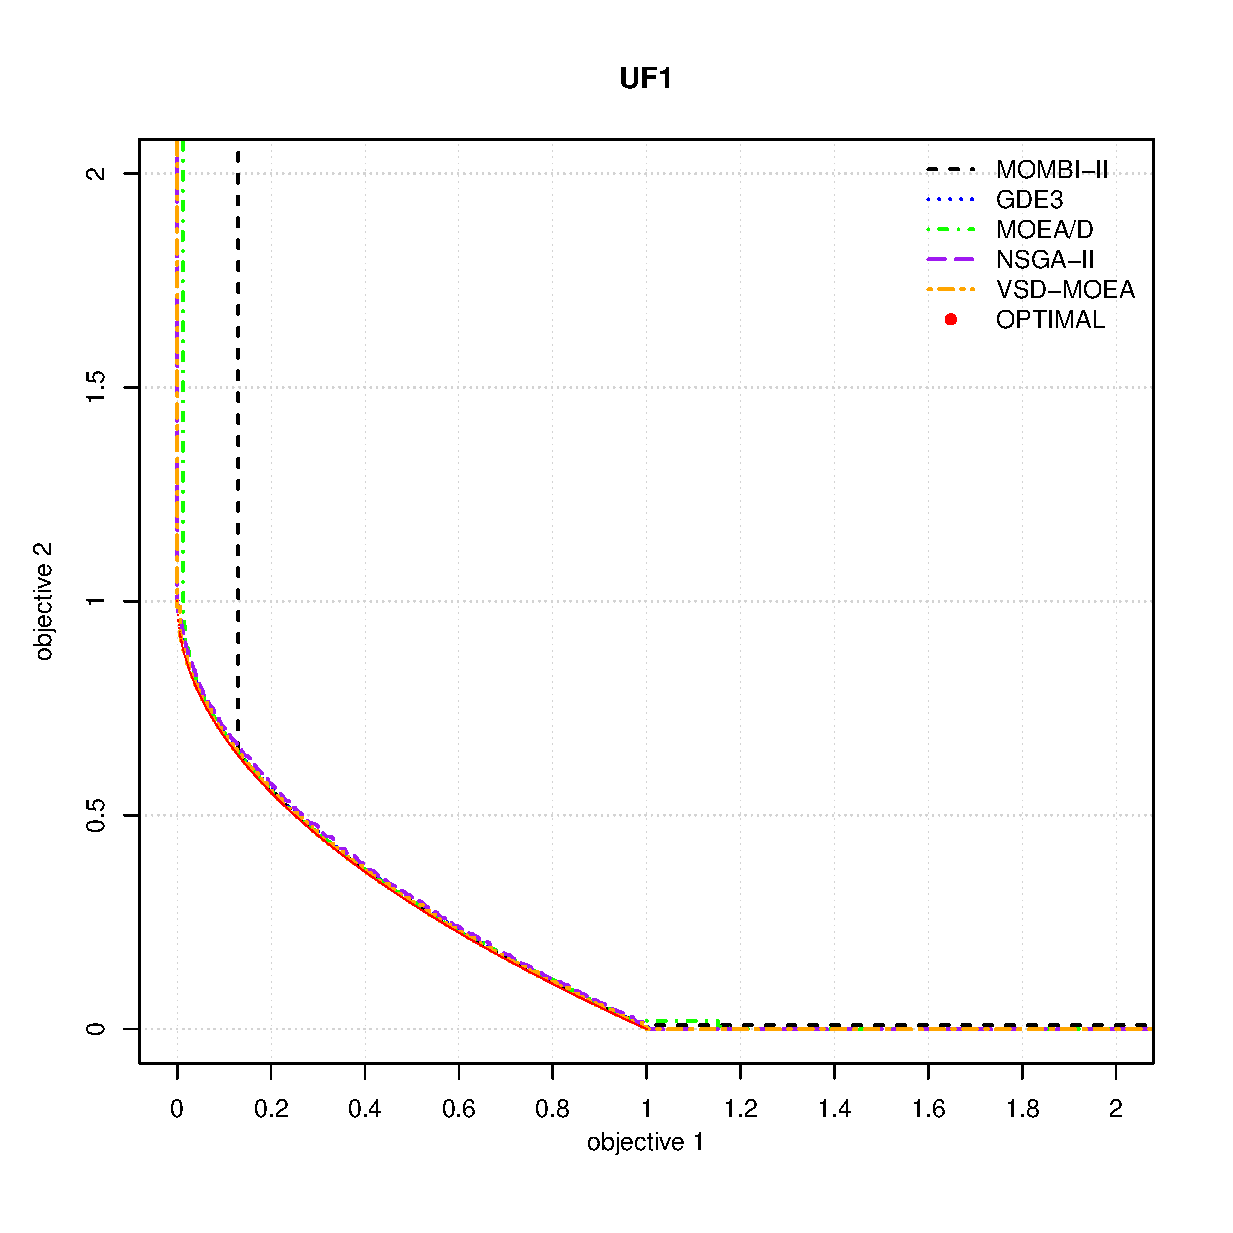
\includegraphics[scale=0.5]{Figures_Chapter2/UF1.eps} & 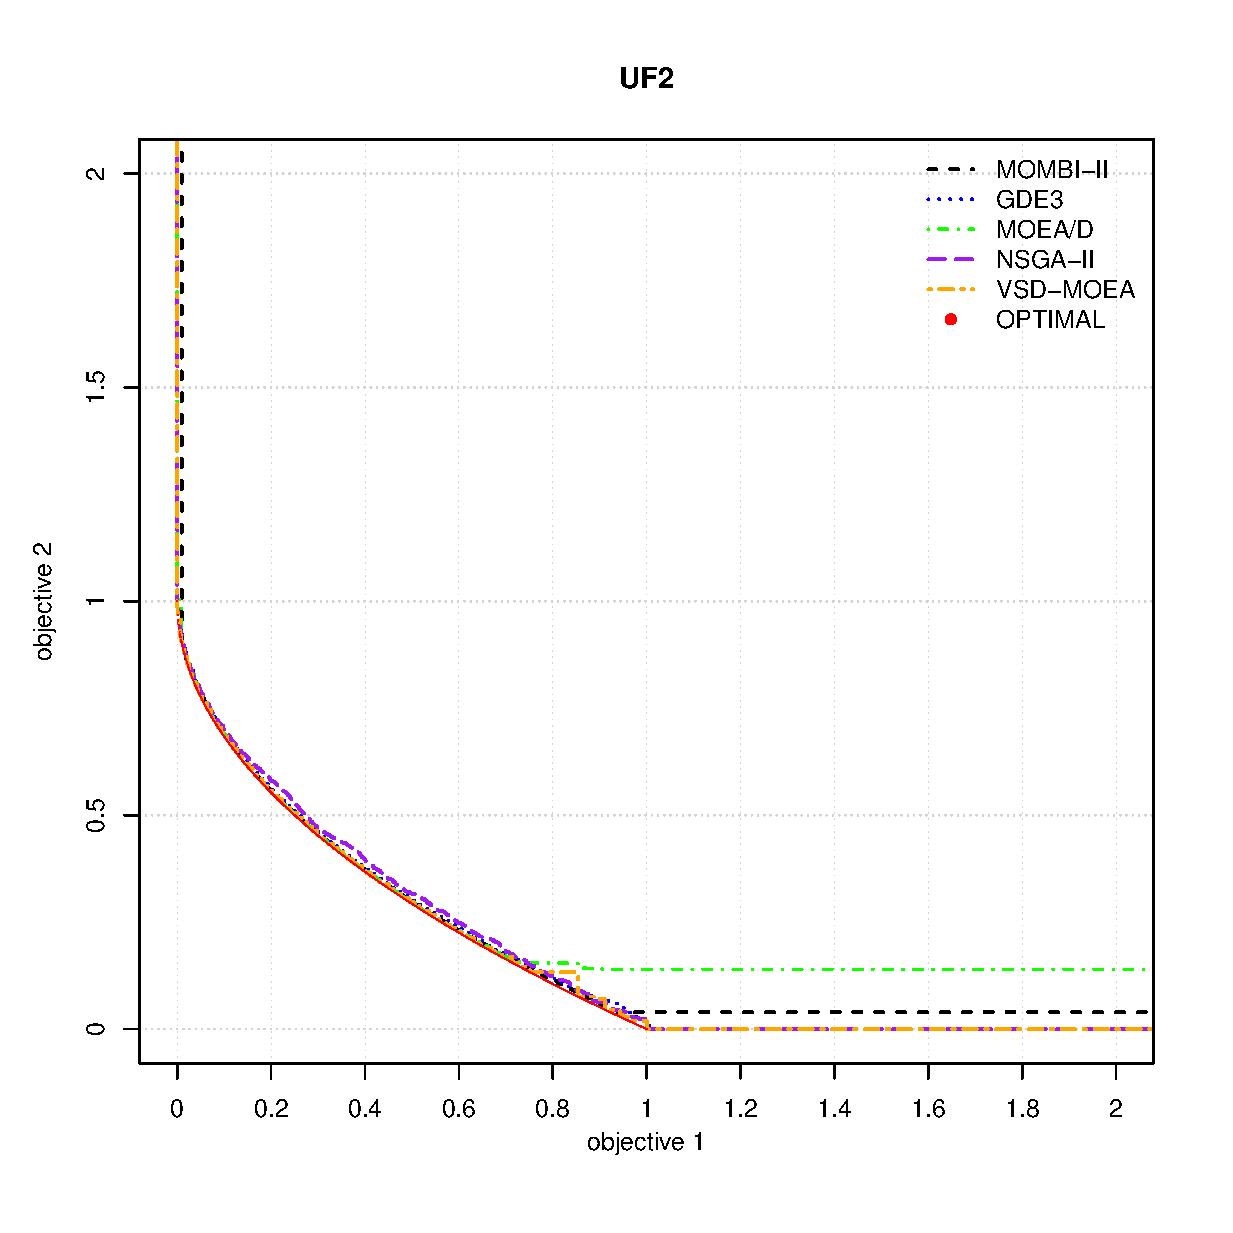
\includegraphics[scale=0.5]{Figures_Chapter2/UF2.eps} \\
UF3 & UF4 \\
\includegraphics[scale=0.5]{Figures_Chapter2/UF3.eps} & 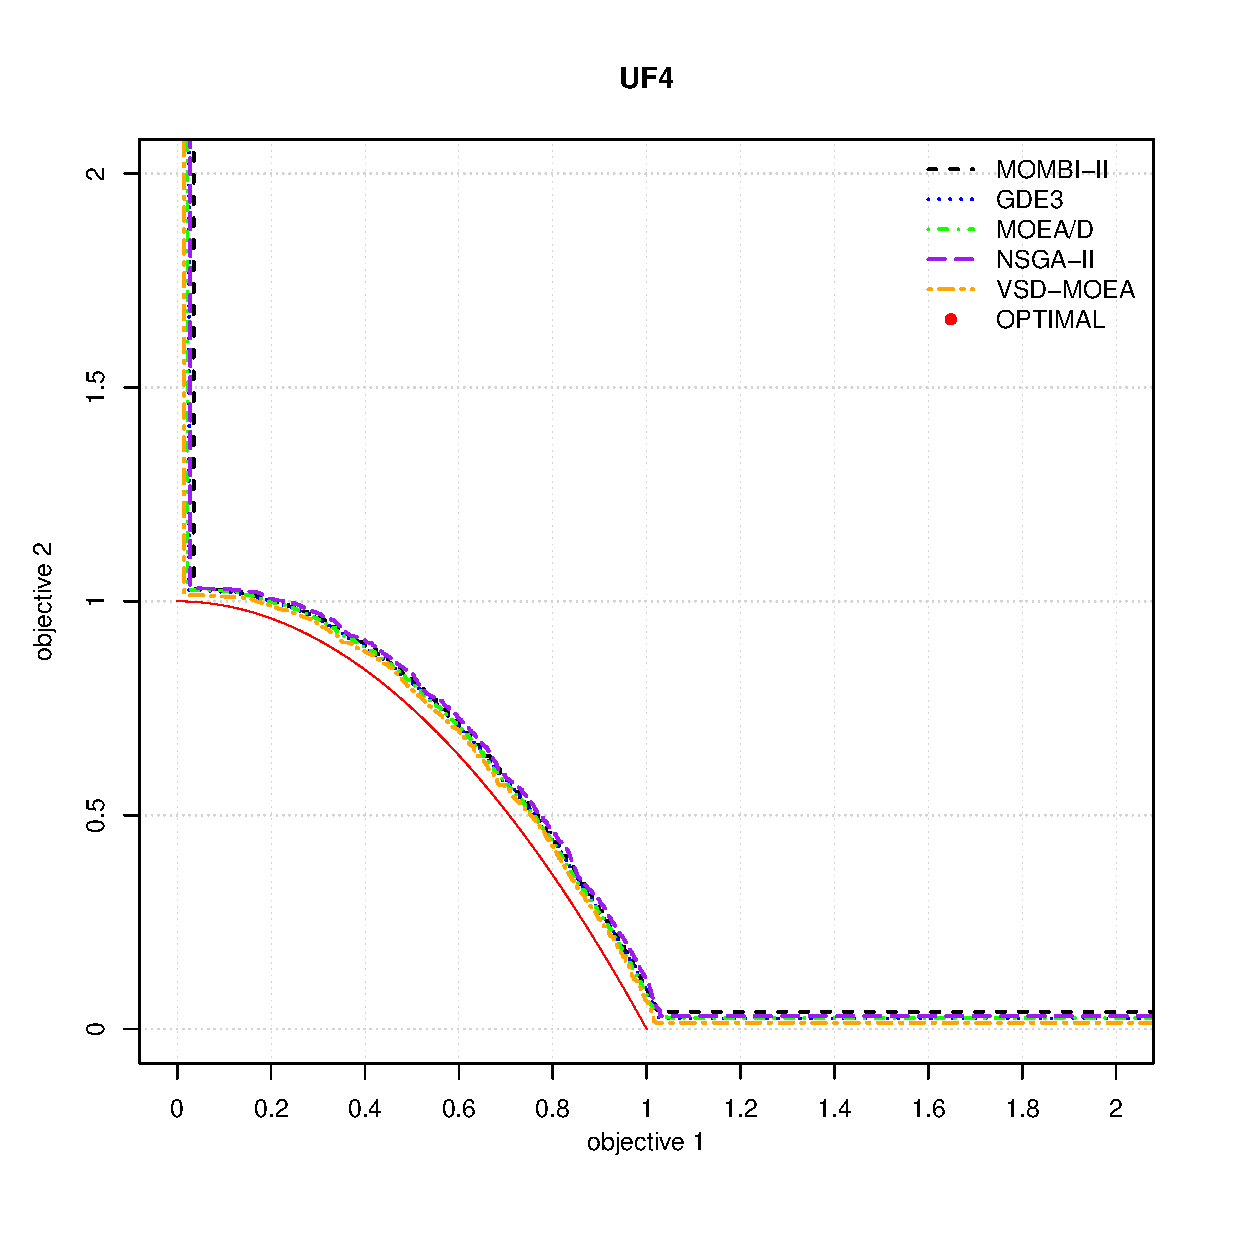
\includegraphics[scale=0.5]{Figures_Chapter2/UF4.eps} \\
UF5 & UF6 \\
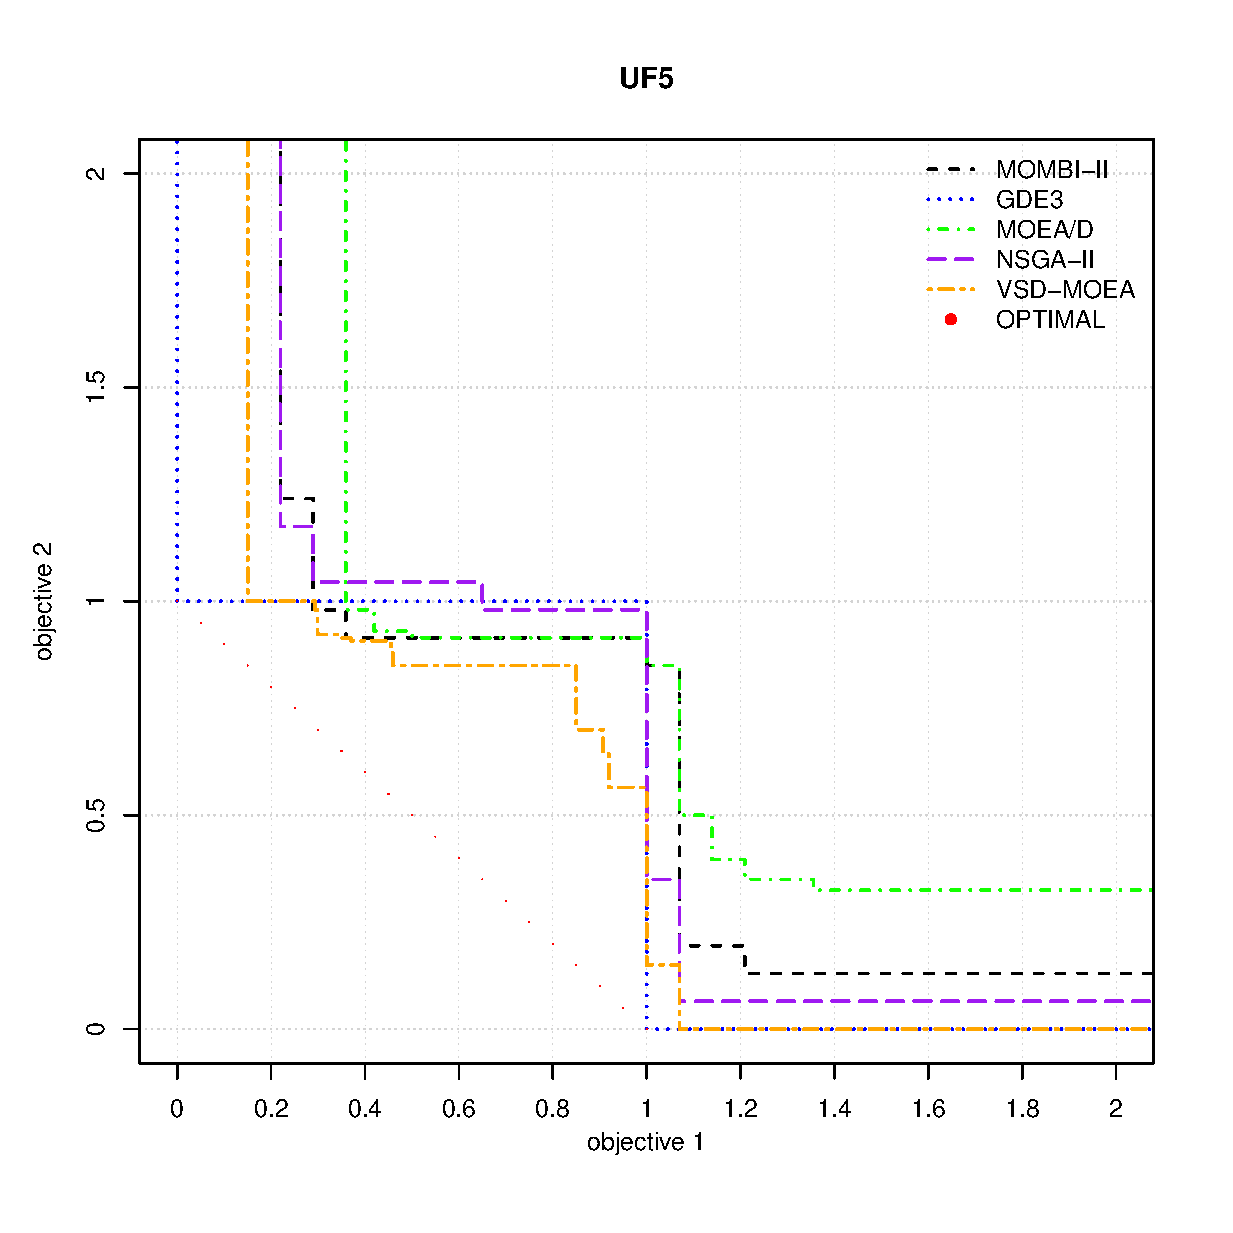
\includegraphics[scale=0.5]{Figures_Chapter2/UF5.eps} & 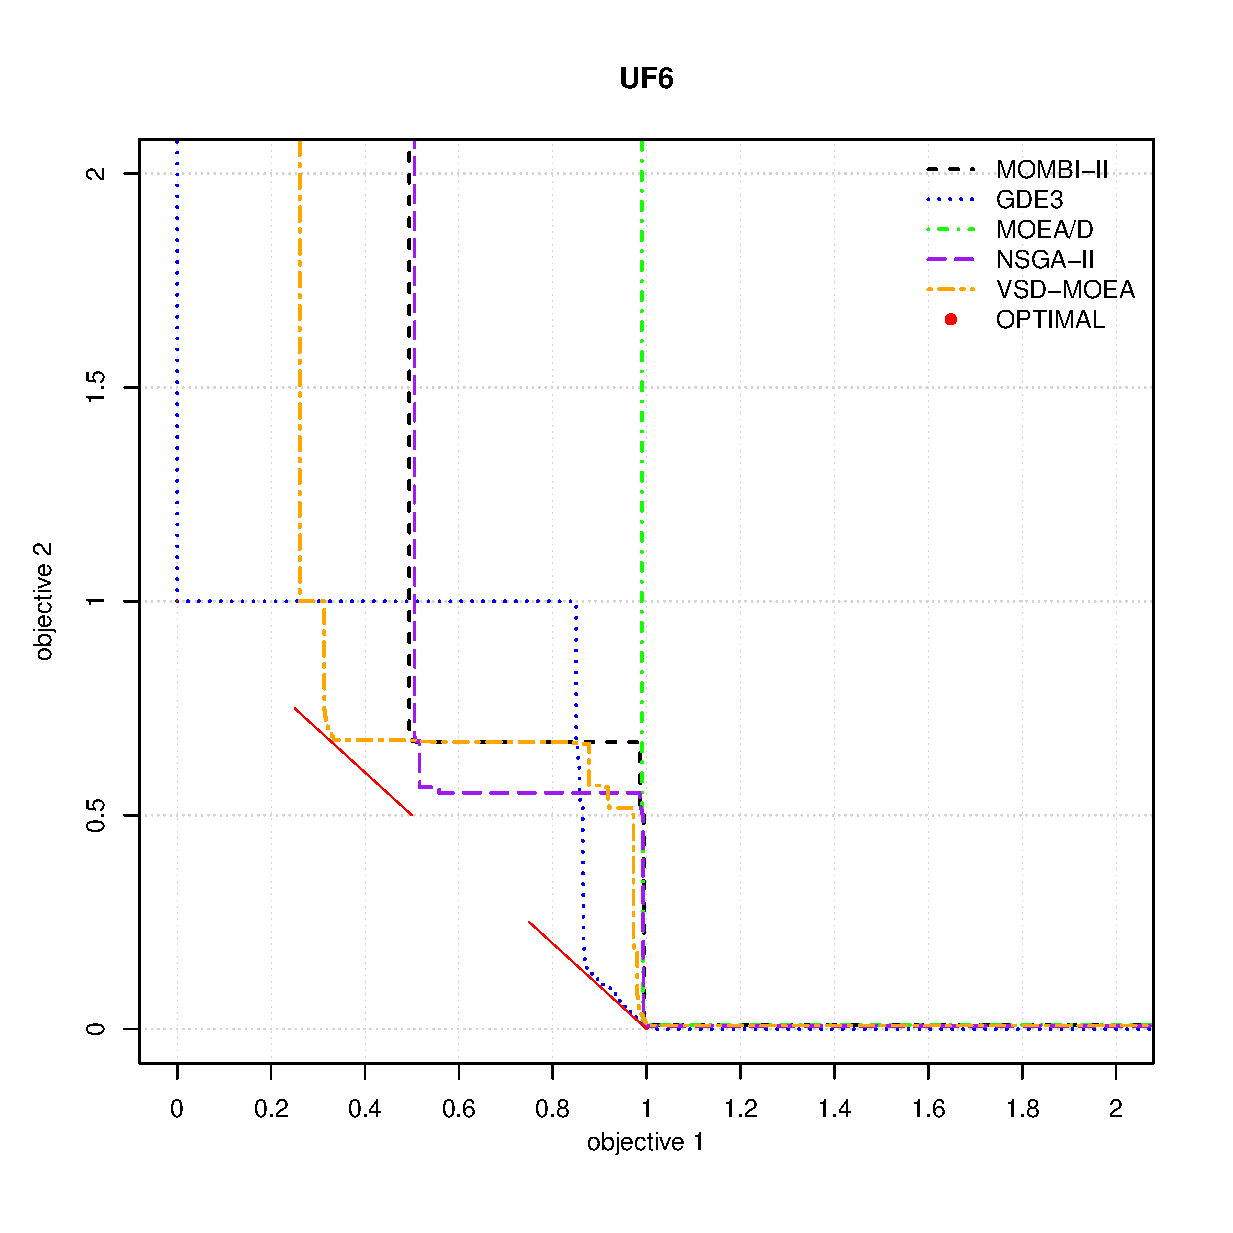
\includegraphics[scale=0.5]{Figures_Chapter2/UF6.eps} \\
UF7 & UF8 \\
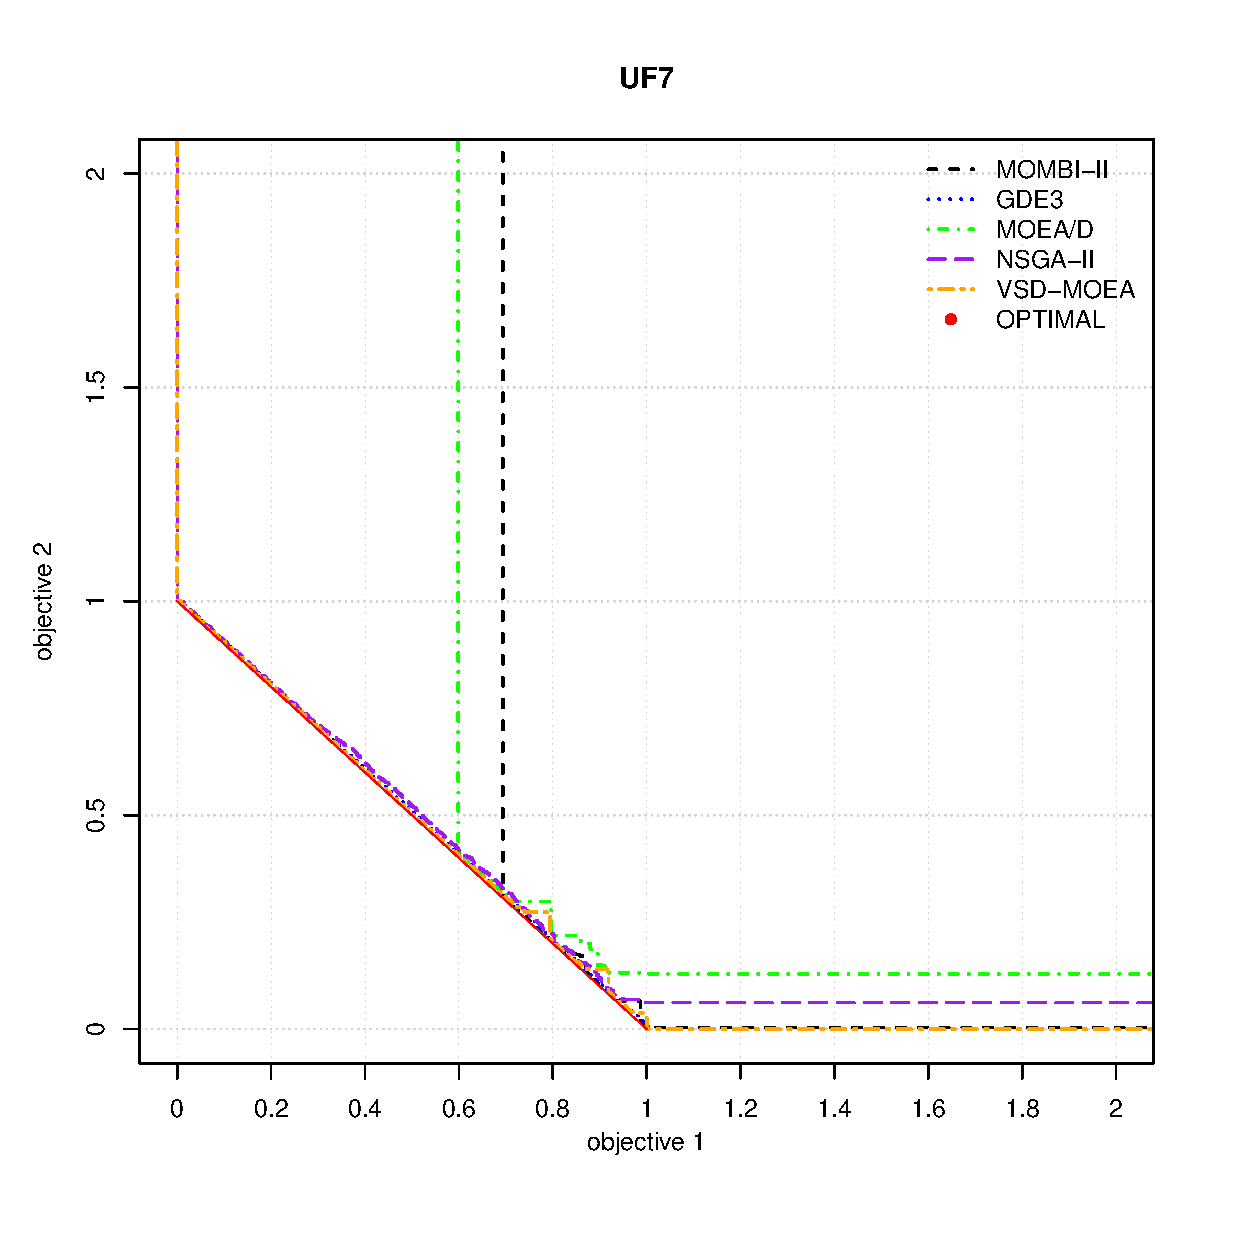
\includegraphics[scale=0.5]{Figures_Chapter2/UF7.eps} & \includegraphics[scale=0.5]{Figures_Chapter2/UF8.eps} \\
UF9 & UF10 \\
\includegraphics[scale=0.5]{Figures_Chapter2/UF9.eps} & \includegraphics[scale=0.5]{Figures_Chapter2/UF10.eps}
\end{tabular}%
}
\end{table}


% Please add the following required packages to your document preamble:
% \usepackage{graphicx}
\begin{table}[]
\centering
\caption{Problemas de prueba UF (CEC 2009)}
\label{tab:UF}
\resizebox{\textwidth}{!}{%
\begin{tabular}{|l|l|c|}
\hline
\multicolumn{1}{|c|}{Nombre} & \multicolumn{1}{c|}{Problema} & Dominio \\ \hline
UF1 & \begin{tabular}[c]{@{}l@{}}$ \begin{array}{lll} f_1&= x_1 + \frac{2}{|J_1|} \sum_{j \in J_1} [x_j - sin(6 \pi x_1 + \frac{j \pi}{n})]^2 \\  f_2 &= 1 - \sqrt{x_1} + \frac{1}{|J_2|} \sum_{j \in J_2} [x_j - sin( 6 \pi x_1 + \frac{j \pi}{n})]^2  \end{array}$\\ $J_1 = \{ j|j$ es impar y $2 \leq j \leq n \}$\\  $J_2 = \{ j|j$ es par con $2 \leq j \leq n \}$\end{tabular} & $[0, 1] \times [-1,1]^{n-1}$ \\ \hline
UF2 & \begin{tabular}[c]{@{}l@{}}$ \begin{array}{lll}f_1 &= x_1 + \frac{2}{|J_1|} \sum_{j \in J_1} y_j^2  \\ f_2 &= 1 - \sqrt{x_1} + \frac{1}{|J_2|} \sum_{j \in J_2} y_j^2,\end{array}$\\ $J_1$ y $J_2$ son los mismos que en UF1\\ $\begin{array}{lll}y_j =\begin{cases} x_j - [0.3x_1^2 cos(24 \pi x_1 + \frac{4 j \pi}{n}) + 0.6 x_1] cos( 6 \pi x_1 + \frac{j \pi}{n}) \quad j \in J_1 \\x_j - [0.3x_1^2 cos(24 \pi x_1 + \frac{4 j \pi}{n}) + 0.6 x_1] cos( 6 \pi x_1 + \frac{j \pi}{n}) \quad j \in J_2,\end{cases} \end{array}$\end{tabular} & $[0, 1] \times [-1,1]^{n-1}$ \\ \hline
UF3 & \begin{tabular}[c]{@{}l@{}}$\begin{array}{lll} f_1 &= x_1 + \frac{2}{|J_1|} ( 4 \sum_{j \in J_1} y_j^2 - 2 \prod_{j \in J_1} cos (\frac{20 y_j \pi}{ \sqrt[]{j}} ) + 2 ) \\  \\ f_2 &= 1 - \sqrt[]{x_1} + \frac{2}{|J_2|} ( 4 \sum_{j \in J_2} y_j^2 - 2 \prod_{j \in J_2} cos (\frac{20 y_j \pi}{ \sqrt[]{j}} ) + 2 ) \\ y_j &= x_j -  x_1^{ 0.5(1.0 + \frac{3(j-2)}{n-2}) }, \quad j=2, ..., n,\end{array}$\end{tabular} & $[0, 1]^n$ \\ \hline
UF4 & \begin{tabular}[c]{@{}l@{}}$\begin{array}{lll}\\ f_1&= x_1 + \frac{2}{|J_1|} \sum_{j \in J_1} h(y_j)\\ f_2&= 1 - x_1^2 + \frac{2}{|J_2|} \sum_{j \in J_2} h(y_j),\end{array}$\\ $J_1$ y $J_2$ son los mismos que en UF1\\ $\begin{array}{lll} y_j = x_j - sin( 6 \pi x_1 + \frac{j \pi}{ n} ), j=2, ..., n. \\ h(t) = \frac{|t|}{ 1 ++ e^{2 |t| }} \end{array}$\end{tabular} & $[0, 1] \times [-2,2]^{n-1}$ \\ \hline
UF5 & \begin{tabular}[c]{@{}l@{}}$\begin{array}{lll} f_1 &= x_1 +(\frac{1}{2N} + \epsilon) | sin(2 N \pi x_1) + \frac{2}{|J_1|} \sum_{j \in J_1} h(y_j)\\   f_2 &= 1 - x_1 + (\frac{1}{2N} + \epsilon) | sin(2 N \pi x_1) + \frac{2}{|J_2|} \sum_{j \in J_2} h(y_j) \end{array}$\\ $J_1$ y $J_2$ son los mismos que en UF1\\ $\begin{array}{lll} y_j = x_j - sin( 6 \pi x_1 + \frac{j \pi}{ n} ), j=2, ..., n.\\ h(t) = 2t^2 - cos(4 \pi t) + 1 \end{array}$\end{tabular} & $[0, 1] \times [-1,1]^{n-1}$ \\ \hline
UF6 & \begin{tabular}[c]{@{}l@{}}$\begin{array}{lll} f_1 &= x_1 + max \{ 0,2(\frac{1}{2N} + \epsilon ) sin(2N \pi x_1)\} +\\  &\frac{2}{|J_1|} ( 4 \sum_{j \in J_1} y_j^2 - 2 \prod_{j \in J_1} cos( \frac{20 y_j \pi}{\sqrt[]{j}} ) + 2)\\  f_2 &= 1 - x_1 + max \{ 0,2(\frac{1}{2N} + \epsilon ) sin(2N \pi x_1),\} +\\ & \frac{2}{|J_2|} ( 4 \sum_{j \in J_2} y_j^2 - 2 \prod_{j \in J_2} cos( \frac{20 y_j \pi}{\sqrt[]{j}} ) + 2)\end{array}$\\ $J_1$ y $J_2$ son los mismos que en UF1\\ $y_j= x_j - sin(6 \pi x_1 + \frac{j \pi}{n}), j=2,...,n.$\end{tabular} & $[0, 1] \times [-1,1]^{n-1}$ \\ \hline
UF7 & \begin{tabular}[c]{@{}l@{}}$\begin{array}{lll}\\ f_1 &= \sqrt[5]{x_1} + \frac{2}{|J_1|} \sum_{j \in J_1} y_j^2 \\ f_2 &= 1 - \sqrt[5]{x_1} + \frac{2}{|J_2|} \sum_{j \in J_2} y_j^2,\end{array}$\\ $J_1$ y $J_2$ son los mismos que en UF1\\ $y_j = x_j - sin(6 \pi x_1 + \frac{j \pi}{n} ), j=2,..., n$\end{tabular} & $[0, 1] \times [-1,1]^{n-1}$ \\ \hline
UF8 & \begin{tabular}[c]{@{}l@{}}$\begin{array}{lll}f_1 &= cos(0.5 x_1 \pi) cos(0.5 x_2 \pi ) + \frac{2}{|J_1|} \sum_{j \in J_1} (x_j - 2 x_2 sin(2\pi x_1 + \frac{j \pi}{n}))^2 \\ f_2 &= cos(0.5 x_1 \pi) sin(0.5 x_2 \pi ) + \frac{2}{|J_2|} \sum_{j \in J_1} (x_j - 2 x_2 sin(2\pi x_1 + \frac{j \pi}{n}))^2  \\ f_3 &= sin(0.5 x_1 \pi ) + \frac{2}{|J_3|} \sum_{j \in J_1} (x_j - 2 x_2 sin(2\pi x_1 + \frac{j \pi}{n}))^2 \end{array}$\\ $J_1 = \{ j|3 \leq j \leq n \}$, y $j-1$ es una multiplicación de 3, \\ $J_2 = \{ j|3 \leq j \leq n \}$, y $j-2$ es una multiplicación de 3\\ $J_3 = \{ j|3 \leq j \leq n \}$, y $j$ es una multiplicación de 3.\end{tabular} & $[0,1]^2 \times [-2, 2]^{n-2}$ \\ \hline
UF9 & \begin{tabular}[c]{@{}l@{}}$\begin{array}{lll}\\ f_1 &= 0.5[ max\{ 0,(1 + \epsilon) (1 - 4(2 x_1 - 1)^2 ) \} + 2 x_1] x_2 + \\ &\frac{2}{|J_1|} \sum_{j \in J_1} ( x_j - 2 x_2 sin(2 \pi x_1 + \frac{j \pi}{n}) )^2\\ f_2 &= 0.5[ max\{ 0,(1 + \epsilon) (1 - 4(2 x_1 - 1)^2 ) \} - 2 x_1 + 2] x_2 + \\ &\frac{2}{|J_2|} \sum_{j \in J_2} ( x_j - 2 x_2 sin(2 \pi x_1 + \frac{j \pi}{n}) )^2\\ f_3 &= 1 - x_2 + \frac{2}{|J_3|} \sum_{j \in J_3} ( x_j - 2 x_2 sin(2 \pi x_1 + \frac{j \pi}{n}) )^2,\end{array}$\\ $J_1$, $J_2$ y $J_3$ son los mismos que en UF9\\ $\epsilon = 0.1$\end{tabular} & $[0,1]^2 \times [-2, 2]^{n-2}$ \\ \hline
UF10 & \begin{tabular}[c]{@{}l@{}}$\begin{array}{lll}f_1 &= cos(0.5 x_1 \pi ) cos(0.5 x_2 \pi) + \frac{2}{|J_1|} \sum_{j \in J_1} [ 4 y_j^2 - cos( 8 \pi y_j) + 1] \\ f_2 &= cos(0.5 x_1 \pi ) sin(0.5 x_2 \pi) + \frac{2}{|J_2|} \sum_{j \in J_2} [ 4 y_j^2 - cos( 8 \pi y_j) + 1] \\ f_3 &= sin(0.5 x_1 \pi) + \frac{2}{|J_3|} \sum_{j \in J_3} [ 4 y_j^2 - cos( 8 \pi y_j) + 1]\end{array}$\\ $J_1$, $J_2$ y $J_3$ son los mismos que en UF9\\ $y_j = x_j - 2 x_2 sin( 2 \pi x_1 + \frac{j \pi}{n}), \quad j=3, ..., n$\end{tabular} & \multicolumn{1}{l|}{$[0,1]^2 \times [-2, 2]^{n-2}$} \\ \hline
\end{tabular}%
}
\end{table}


%% Please add the following required packages to your document preamble:
%% \usepackage{graphicx}
%\begin{table}[]
%\centering
%\caption{My caption}
%\label{my-label}
%\resizebox{\textwidth}{!}{%
%\begin{tabular}{|c|l|c|}
%\hline
%Nombre & \multicolumn{1}{c|}{Problema} & Dominio de los parámetros \\ \hline
%ZDT1 & $ \begin{array}{lll} f_1(x_1) &= x_1 \\g(x_2, ..., x_n) &= 1+9,\sum_{i=2}^n x_i / (n-1) \\h(f_1, g) &= 1 - \sqrt{f_1/g} \end{array}$ & $[0,1]$ \\ \hline
%ZDT2 & Igual que ZDT1, a excepción de $h = 1-(f_1 / g)^2$ & $[0,1]$ \\ \hline
%ZDT3 & Igual que ZDT1, a excepción de $h(f_1, g) = 1 - \sqrt{f_1/g} - (f_1 / g) sin( 10 \pi f_1)$ & $[0,1]$ \\ \hline
%ZDT4 & Igual que ZDT1, a excepción de $h(f_1, g) = 1 - \sqrt{f_1/g}$ & $ \begin{array}{lll}  x_1 \in [0,1] \\ x_2, ..., x_n \in [-5, 5] \end{array}$ \\ \hline
%ZDT6 & $ \begin{array}{lll} f_1(x_1) &= 1 - exp(-4 x_1) sin^6 (6 \pi x_1) \\g(x_2, ..., x_n) &= 1 + 9 \sum_{i=2}^n (x_i / (n-1))^{0.25} \\h(f_1, g) &= 1 - (f_1/g)^2 \end{array}$ & $[0,1]$ \\ \hline
%DTLZ1 & $ \begin{array}{lll}  f_1 &= (1+g) 0.5 \prod_{i=1}^{M-1} x_i \\ f_{m=2:M-1} &= (1+g) 0.5 (\prod_{i=1}^{M-m} x_i)(1 - y_{M-m+1}) \\ f_M &= (1+g) 0.5 (1-x_1) \\ g &= 100[x_M+\sum_{x_i \in x_M} (  (x_i - 0.5)^2 - cos(20 \pi (x_i - 0.5)) )] \end{array}$ & $[0,1]$ \\ \hline
%DTLZ2 & $ \begin{array}{lll}   f_1 &= (1+g) \prod_{i=1}^{M-1} cos(x_i \pi/2) \\   f_{m=2:M-1} &= (1+g) \left (  \prod_{i=1}^{M-m} cos(x_i \pi / 2)   \right ) sin(x_{M-m+1} \pi / 2)   \\   f_M &= (1+g) sin(x_1 \pi /2) \\   g &= \sum_{x_i \in x_M} (x_i -0.5)^2 \end{array}$ & $[0,1]$ \\ \hline
%DTLZ3 & Igual que DTLZ2, excepto que se utiliza la ecuación $g$ del DTLZ1 & $[0,1]$ \\ \hline
%DTLZ4 & Igual que DTLZ2, excepto que $x_i \in x$ es reemplazado por $x_i ^ \alpha$, donde $\alpha > 0$ & $[0,1]$ \\ \hline
%DTLZ5 & Igual que DTLZ2, excepto que $x_2, ..., x_{M-1} \in x $ son reemplazados por $\frac{1+2 g x_i}{2(1+g)}$ & $[0,1]$ \\ \hline
%DTLZ6 & Igual que DTLZ5, excepto que la ecuación para $g$ es reemplazada por $g = \sum_{x_i \in x_M} x_i^{0.1}$ & $[0,1]$ \\ \hline
%DTLZ7 & $ \begin{array}{lll} f_{m=1:M-1} &= x_m \\ f_M &= (1+g) \left (  M - \sum_{i=1}^{M-1} \left [ \frac{f_i}{1+g}(1 + sin(3 \pi f_i)) \right ] \right) \\ g &= 1+9 \sum_{x_i \in x_M} x_i /k \end{array}$ & $[0,1]$ \\ \hline
%\multicolumn{1}{|l|}{WFG1} & \begin{tabular}[c]{@{}l@{}}$\begin{array}{lll}      t^1_{i=1:k} &= x_i \\ t^1_{k+1:n} &= s\_linear(x_i, 0,35) \\ t^2_{i=1:k} &= x_i \\ t^2_{i=k+1:n} &= b\_flat(x_i, 0.8, 0.75, 0.85) \\ t^3_{i=1:n} &= b\_poly(x_i, 0.02) \\ t^4_{i=1:M-1} &= r\_sum(  \{ x_{(i-1)k/(M-1)+1},...,y_{ik/(M-1)} \}, \\  &\{ 2((i-1)k/(M-1)+1), ..., 2ik/(M-1) \} ) \\ t^4_M &= r\_sum( \{x_{k+1},...,y_n\}, \{ 2(k+1), ..., 2n \}) \\ h_{m=1:M-1} &= convex_m\\ \end{array}$\end{tabular} & $[0, 2 i]$ \\ \hline
%\multicolumn{1}{|l|}{WFG2} & \begin{tabular}[c]{@{}l@{}}Implementar $t^1$ del WFG1\\ $ \begin{array}{lll} t^2_{i=1:k}  &= x_i\\    t^2_{i =k+1:k+l/2} &= r\_nonsep(\{ x_{k+2(i-k)-1}, z_{k+2(i-k)}  \}, 2 )\\    t^3_{i=1:M-1} &= r\_sum( \{  x_{(i-1)k / (M-1) +1}, ..., x_{ik / (M-1)}  \}, \{1,...,1\} )\\    t^3_M &= r\_sum( \{ y_{k+1},..., y_{k+l/2}  \},\{1,...,1\} )\\    h_{m=1:M-1} &= convex_m\\    h_M &= disc_M ( \alpha = \beta =1, A = 5)\\  \end{array}$\end{tabular} & $[0, 2 i]$ \\ \hline
%\multicolumn{1}{|l|}{WFG3} & \begin{tabular}[c]{@{}l@{}}Implementar $t^1$, $t^2$ y $t^3$ del WFG2\\ $h_{m=1:M} = linear_m$\end{tabular} & $[0, 2 i]$ \\ \hline
%\multicolumn{1}{|l|}{WFG4} & \begin{tabular}[c]{@{}l@{}}$\begin{array}{lll}  t^1_{i=1:n} &= s\_multi(x_i, 30, 10, 0.35)\\   t^2_{i=1:M-1} &= r\_sum(\{ x_{(i-1)k / (M-1)+1},..., x_{ik / (M-1)}  \}, \{1,...,1\})\\   t^2_M &= r\_sum( \{ x_{k+1}, ..., x_n  \}, \{1,...,1\})\\   h_{m=1:M} &= concave_m\\ \end{array}$\end{tabular} & $[0, 2 i]$ \\ \hline
%\multicolumn{1}{|l|}{WFG5} & \begin{tabular}[c]{@{}l@{}}$t^1_{i=1:n} = s\_decept(x_i, 0.35, 0.001, 0.05)$\\ Implementar $t^2$ del WFG4 \\ $h_{m=1:M} &= concave_m$\end{tabular} & $[0, 2 i]$ \\ \hline
%\multicolumn{1}{|l|}{WFG6} & \begin{tabular}[c]{@{}l@{}}Implementar $t^1$ del WFG1\\ $\begin{array}{lll} t^2_{i=1:M-1} &= r\_nonsep(\{y_{(i-1)k / (M-1) +1}, ..., y_{ik / (M-1)}\}, k/(M-1))\\  t^2_M &= r\_nonsep(\{ y_{k+1}, ..., y_n \}, l)\\ h_{m=1:M} &=concave_m\\  \end{array}$\end{tabular} & $[0, 2 i]$ \\ \hline
%\multicolumn{1}{|l|}{WFG7} & \begin{tabular}[c]{@{}l@{}}$\begin{array}{lll} t^1_{i=1:k} &= b\_param(x_i, r\_sum(\{ x_{i+1}, ..., x_n \},\{1,...,1\}), \frac{0.98}{49.88}, 0.02, 50)\\    t^1_{i=k+1:n} &=x_i\\    \end{array}$\\ Implementar $t^1$ del WFG1\\ Implementar $t^2$ del WFG4\\ $h_{m=1:M} = concave_m$\end{tabular} & $[0, 2 i]$ \\ \hline
%\multicolumn{1}{|l|}{WFG8} & \begin{tabular}[c]{@{}l@{}}$\begin{array}{lll}   t^1_{i=1:k} &= x_i\\    t^1_{k+1:n} &= b\_param( x_i, r\_sum( \{ x_1,, ...., x_{i-1} \}, \{ 1,..., 1\} ) , \frac{0.98}{49.98}, 0.02, 50)\\   \end{array}$\\ Implementar $t^2$ del WFG1\\ Implementar $t^2$ del WFG4\\ $h_{m=1:M} = concave_m$\end{tabular} & $[0, 2 i]$ \\ \hline
%\multicolumn{1}{|l|}{WFG9} & \begin{tabular}[c]{@{}l@{}}$\begin{array}{lll}t^1_{i=1:n-1} &= b\_param( x_i, r\_sum(  \{ y_{i+1}, ..., y_n \}, \{1,...,1\} ), \frac{0.98}{49.98}, 0.02, 50 )\\ t^1_{n} &= x_n\\ t^2_{i=1:k} &= s\_decept(x_i, 0.35, 0.001, 0.05)\\ t^2_{i=k+1:n} &= s\_multi(x_i, 30, 95, 0.35)\\ \end{array}$\\ Implementar $t^2$ del WFG6\\ $h_{m=1:M} = concave_m$\end{tabular} & $[0, 2 i]$ \\ \hline
%\end{tabular}%
%}
%\end{table}
%


% Please add the following required packages to your document preamble:
% \usepackage{graphicx}
\begin{table}[H]
\centering
\caption{Propiedades de los problemas de prueba ZDT, DTLZ, WFG y UF}
\label{tab:Propiedades}
\resizebox{\textwidth}{!}{%
\begin{tabular}{|c|c|c|c|c|c|}
\hline
\textbf{Nombre} & \textbf{Separable} & \textbf{Modalidad} & \multicolumn{1}{l|}{\textbf{Geometría del frente de Pareto}} & \multicolumn{1}{l|}{\textbf{Distribución de las soluciones}} & \textbf{Número de objetivos} \\ \hline
ZDT1 & Si & Unimodal & Convexo & Uniforme & 2 \\ \hline
ZDT2 & Si & Unimodal & Concavo & Uniforme & 2 \\ \hline
ZDT3 & Si & Unimodal-Multimodal & Desconectado & Uniforme & 2 \\ \hline
ZDT4 & Si & Unimodal-Multimodal & Convexo & Uniforme & 2 \\ \hline
ZDT6 & Si & Multimodal & Concavo & Polinomial & 2 \\ \hline
DTLZ1 & Si & Multimodal & Lineal & Uniforme & N \\ \hline
DTLZ2 & Si & Unimodal & Concavo & Uniforme & N \\ \hline
DTLZ3 & Si & Multimodal & Concavo & Uniforme & N \\ \hline
DTLZ4 & Si & Unimodal & Concavo & Polinomial & N \\ \hline
DTLZ5 & - & Unimodal & Degenerado - Arco & Uniforme & N \\ \hline
DTLZ6 & - & Unimodal & Degenerado - Arco & Depende del parámetro & N \\ \hline
DTLZ7 & Si & Unimodal-Multimodal & Desconectado - Mixto & Uniforme & N \\ \hline
WFG1 & Si & Unimodal & Convexo - Mixto & Polinomial - Regiones planas & N \\ \hline
WFG2 & No & Unimodal-Multimodal & Convexo - Desconectado & Uniforme & N \\ \hline
WFG3 & No & Unimodal & Lineal - Degenerado & Uniforme & N \\ \hline
WFG4 & Si & Multimodal & Concavo & Uniforme & N \\ \hline
WFG5 & Si & Deceptivo & Concavo & Uniforme & N \\ \hline
WFG6 & No & Unimodal & Concavo & Uniforme & N \\ \hline
WFG7 & Si & Unimodal & Concavo & Depende del parámetro & N \\ \hline
WFG8 & No & Unimodal & Concavo & Depende del parámetro & N \\ \hline
WFG9 & No & Unimodal-Deceptivo & Concavo & Depende del parámetro & N \\ \hline
UF1 & - & - & Concavo & - & 2 \\ \hline
UF2 & - & - & Concavo & - & 2 \\ \hline
UF3 & - & - & Concavo & - & 2 \\ \hline
UF4 & - & - & Convexo & - & 2 \\ \hline
UF5 & - & - & Frente de 21 puntos & - & 2 \\ \hline
UF6 & - & - & Lineal & - & 2 \\ \hline
UF7 & - & - & Lineal & - & 2 \\ \hline
UF8 & - & - & Parabólico & - & 3 \\ \hline
UF9 & - & - & Planar & - & 3 \\ \hline
UF10 & - & - & Parabólico & - & 3 \\ \hline
\end{tabular}%
}
\end{table}

\subsection{Generar las soluciones óptimas}
Generar las soluciones óptimas de Pareto que corresponden a los problemas de prueba es un aspecto importante, ya que varias métricas utilizan estas soluciones óptimas como conjuntos de referencia.
%
Aunque se proporcionan las fórmulas para obtener los óptimos de pareto en los problemas multi-objetivo, se debe tener cuidado, principalmente porque una distribución de soluciones en el espacio de las variables no determina una distribución igual en el espacio objetivo, tal es el caso de los problemas WFG, que aunque proporcionan un generador de soluciones, las soluciones no tienen una distribución adecuada, principalmente en configuraciones que aumentan la complejidad.
%
Además la cantidad de puntos de referencia es afectado en caso de que el número de objetivos o el número de variables es elevado, ya que al generar puntos en base a una distribución uniforme podría no ser suficiente para representar adecuadamante al frente de Pareto.
%
Para resolver estos inconvenientes se implementa un método Quasi aleatorio, específicamente el método de Hammersley el cual produce una secuencia de números con baja discrepancia \citep{Joel:Hammersley, Joel:AlgoritmoHungaro}.
%
A diferencia de un generador de números aleatorios, implementar una secuencia de baja discrepancia genera puntos en el espacio de un modo más sistemático.
%
Ya que un clásico generador aleatorio, una misma área puede explorarse varias veces y otras no ser exploradas nunca, particularmente esta dificultad se incrementa considerablemente al aumentar la dimensión de los espacios.
%
El procedimiento que sugerido consiste en generar una secuencia de números en el espacio de soluciones óptimas por medio del método de Hammersley, posteriormente se implementa un proceso de filtrado, el cual consite en elimintar a los puntos más cercanos dada una tolerancia. 
%
Como se puede observar en la figura \ref{fig:Random} la cual es resultado de generar diez mil puntos en un espacio de tres dimensiones, en la parte izquierda de la fiigura los puntos se generan por medio de una distribución uniforme y en la parte derecha se generan por medio del método de hammersley, se puede observar que generar datos con una distribución uniforme puede provocar regiones aisladas.

\begin{figure}[H]
\centering
\scriptsize
\includegraphics[scale=0.35]
{Figures_Chapter2/Random.png}
\includegraphics[scale=0.35]
{Figures_Chapter2/Hammersley.png}
\caption{Frente de Pareto problema WFG5, en la izquierda con un método aleatorio y con el método de Hammersley considerando diez mil puntos.}
\label{fig:Random}
\end{figure}


\section{Métricas}
En optimización multi-objetivo, se han desarrollado técnicas para medir el desempeño de las soluciones obtenidas.
%
Se han propuesto varios indicadores para evaluar la calidad del conjunto de soluciones no dominados \citep{Joel:EjemploFallaGD}.\\
%
En general los indicadores son métricas las cuales determinan el grado de convergencia al frente de Pareto y/o la diversidad de las soluciones en el frente de Pareto.
%
El indicador que se utiliza más frecuentemente es el hipervolumen \citep{Joel:ComparativeCaseStudy} . 
%
Esto se debe a que ningún otro indicador es \textit{Pareto compliant} \citep{Joel:HypervolumeRevisited}. 
%
Una característica importante que un indicador debería tener es ser \textit{Pareto compliant} \citep{Joel:ComparacionMetricas}, esto quiere decir que el indicador no debería contradecir el orden inducido por la relación de dominancia.
%
Así, dados dos conjuntos de soluciones $A$ y $B$ si $A \succeq B \land B \nsucc A$, entonces el valor del indicador de $A$ no debe ser peor que el valor del indicador $B$.
%
Para considerarse estrictamente \textit{compliant} se requiere que $A \succeq B \land B  \nsucc A$ implicando que el valor del indicador de $A$ es estrictamente mejor que el valor del indicador $B$, esto es:
\begin{equation*}
   A \succeq B \land B \nsucceq A \Rightarrow  I(A) > I(B)
\end{equation*}
%

%
En la literatura se ha descrito repetidas veces \citep{Joel:HypervolumeRevisited, Joel:EjemploFallaGD}  que con indicadores de tipo Pareto \textit{non-compliant} se pueden obtener resultados engañosos al momento de evaluar al conjunto de soluciones no dominadas. 
%
En el \citeyear{Joel:EjemploFallaGD} \citeauthor{Joel:EjemploFallaGD} demuestran que se pueden obtener resultados engañosos implementando la distancia generacional (GD).
%
En este contexto un conjunto de soluciones óptimas de Pareto se denotan por $P^*$ y el conjunto de aproximaciones por $Q$ compuestos por $M$ y $N$ puntos respectivamente.

\subsection{Distancia Generacional y Distancia Generacional Invertida}

La Distancia Generacional (GD - \cite{Joel:GD}) y la Distancia Generacional Invertida  son indicadores considerados Pareto \textit{non-compliant}, y para ser implementados es requerido el conjunto óptimo de Pareto.
%
El GD está diseñado para obtener la distancia promedio de cada solución al punto de referencia más cercano. 


Por otra parte la Distancia Generacional Invertida (IGD) fue propuesta por \cite{Joel:ParallelizationMOEA, Joel:SwarmOptimizerDiversity}. Sin embargo ya se habían propuesto indicadores similares por \citeauthor{Joel:SimulatedAnnealingMetaheuristic} en \citeyear{Joel:SimulatedAnnealingMetaheuristic}.\\
%
El IGD es la distancia promedio de cada punto de referencia a su solución más cercana.
%
Así, si se tiene un conjunto de puntos utilizados como referencia, los cuales estén bien distribuidos en el frente de Pareto, un valor pequeño del IGD sugiere una buena convergencia de las soluciones al frente de Pareto y una buena distribución en relación al frente de Pareto.
\begin{equation}
\begin{split}
GD (P^*, Q) = \frac{1}{|N|}\left(  \sum_{i=1}^{|N|} d_i^p  \right) ^{1/p} \qquad
IGD (P^*, Q) = \frac{1}{|M|}\left(  \sum_{i=1}^{|M|} \hat{d}_j^p  \right) ^{1/p}
\end{split}
\end{equation}
Donde $d_i$ denota la distancia Euclídea entre la solución $y_i \in Q$ y el punto de referencia más cercano del conjunto $P^*$ y $\hat{d_i}$ denota la distancia entre el punto de referencia $x_i^* \in P^*$ a la solución más cercana del conjunto $Q$. 
% 
Recientemente \citeauthor{Joel:HausdorffDistance} propusieron una modificación al GD y al IGD, donde argumentan que conforme aumenta el número de puntos $M$, la calidad en la aproximación "mejora", aunque la aproximación aparentemente no ha cambiado, tratándose de un falso positivo.
%
Esto es demostrado, asumiendo que el conjunto de distancias $d_i$ (para el caso del GD) sean 1 y dada una muestra de $N$ soluciones, entonces:
\begin{equation*}
  GD(P^*, Q) = \frac{1}{|N|}\left( \sum_{i=1}^{|N|} d_i^p  \right) ^{1/p} = \frac{ \Vert (1,...,1)^T \Vert_p }{N} = \frac{\sqrt[p]{N}}{N} 
\end{equation*}
%
Se puede observar que:
\begin{itemize}
\item Al incrementar el número $N$ de puntos, la calidad que pertenece a la aproximación \textit{mejora} aunque aparentemente no ha cambiado.
\item La secuencia de puntos convergen a una aproximación "perfecta", esto es:
\begin{equation*}
\begin{split}
  \lim_{N \to \infty} GD( P^*, Q) = 0 
\end{split}
\end{equation*}
\end{itemize}
Lo mismo ocurre para el IGD, al considerar más puntos de referencia.
%
Para evitar el efecto mencionado, se propone la modificación al indicador, conocido como la potencia media para promediar las distancias:
\begin{equation}
\begin{split}
& GD_P(P^*, Q) = \left( \frac{1}{|N|}  \sum_{i=1}^{|N|} d_i^p  \right) ^{1/p} = \frac{ \Vert d_i \Vert_p }{\sqrt[p]{N}}  \\
& IGD_P(P^*, Q) = \left( \frac{1}{|M|}  \sum_{i=1}^{|M|} \hat{d}_j^p  \right) ^{1/p} = \frac{ \Vert \hat{d}_j \Vert_p }{\sqrt[p]{N}}  
\end{split}
\end{equation}
%
Esta modificación evita que al aumentar el número de soluciones (en el caso de GD) o al momento de aumentar el número de puntos de referencia (en el caso del IGD) la calidad del indicador se vea afectado.
%

%
Sin embargo como ya se explicó anteriormente al ser estas métricas Pareto \textit{non-compliant}, existen escenarios en que la estimación puede ser cuestionable, por ejemplo en la figura \ref{fig:IGD_Fallo} donde el conjunto de soluciones A y B evaluados con el IGD son 3.71 y 2.59 respectivamente, se observa que aunque el conjunto de soluciones A tenga más puntos cercanos a los  puntos de referencia la estimación de la métrica es mejorado por el conjunto de soluciones B.

\begin{figure}[H]
\centering
\scriptsize
\includegraphics[scale=0.2]
{Figures_Chapter2/IGD_Problema.png}
\decoRule
\caption{Ejemplo con 5 puntos de referencia IGD.}
\label{fig:IGD_Fallo}
\end{figure}
%
En lugar del IGD se propone la distancia generacional invertida modificada (IGD+) propuesta por \citeauthor{Joel:IGDPlus_And_GDPlus} en el \citeyear{Joel:IGDPlus_And_GDPlus}, la cual es considerada como \textit{Weak Pareto compliance}, este indicador consiste en:


\textit{Si una solución es dominada por un punto de referencia, entonces se utiliza la distancia Euclídea sin alguna modificación. Sin embargo, si la solución y el punto de referencia son no dominados entre sí, entonces se calcula la mínima distancia desde el punto de referencia a la región dominada por la solución.}
%

La forma del IGD+ es similar al IGD propuesto previamente, a diferencia que la distancia Euclídea es modificada, de la siguiente manera:
\begin{itemize}
\item En problemas de minimización es \[d^+(z,a) = \sqrt{d_1^2 + ... + d_m^2} = \sqrt{max\{a_1 - z_1, 0\}^2+...+max\{a_m - z_m, 0\}^2}   \]
\item En problemas de maximización es \[d^+(z,a) = \sqrt{d_1^2 + ... + d_m^2} = \sqrt{max\{z_1 - a_1, 0\}^2+...+max\{z_m - a_m, 0\}^2}\]
\end{itemize}
%

\subsection{Distancia promedio de Hausdorff $\Delta_p$}
La distancia de Hausdorff $d_H$ es una herramienta utilizada para medir la distancia entre diferentes objetos \cite{Joel:HausdorffDistance}.
%
A excepción de trabajos teóricos, esta distancia no es muy utilizada en el ámbito multi-objetivo, la mayor razón es que probablemente $d_H$ penaliza los valores más atípicos de un conjunto de puntos, lo cual produce que una ``buena'' aproximación que contiene al menos un dato atípico sea considerada como una ``mala'' aproximación.
%
Un forma para remediar esto es promediando las distancias de los elementos que pertenecen a los conjuntos, guiando a una ``distancia promedio de Hausdorff''.
%
\begin{equation}
\Delta_p(P) = max \{ GD_p(P^*, Q), IGD_p(P^*, Q) \}
\end{equation}
%
Los autores \citeauthor{Joel:HausdorffDistance} argumentan que una propiedad importante que debe poseer una métrica es la de satisfacer la desigualdad del triángulo.
%
Sin embargo se debe tener cuidado que al promediar las distancias es posible violar dicha propiedad.
%
El efecto que tiene el parámetro $p$ sobre la métrica $\Delta_p$ es la clave para manejar los datos atípicos, ya que un valor pequeño de $p$ tiene un mayor efecto en el promedio y existe una menor influencia de los datos atípicos.
%
De otra forma, si $p$ es incrementado, los datos atípicos influyen más en la métrica $\Delta_p$.
%
En el caso extremo donde $p \rightarrow \infty$, sólo son consideradas las distancias que corresponden a los puntos más lejanos.
%
En un análisis práctico se concluye que las violaciones de la desigualdad del triángulo disminuyen conforme aumenta el parámetro de $p$, de igual forma sucede como conforme incrementa el número de elementos en los conjuntos considerados.
%
Esto demuestra una razón por los cual en la literatura no se observan análisis sobre la violación de la desigualdad del triángulo.
%
Ya que para usos prácticos se observa que $\Delta_p$ debería ser suficiente ''similar`` a una métrica.


\subsection{Distancia al vecino más cercano - DCN}
El DCN (\textit{Distance to the Closest Neighbor}) es una métrica que normalmente se utiliza en algoritmos evolutivos que mantienen algún mecanismo para gestionar la diversidad \citep{Joel:DCN, Joel:MultiDynamic}.\\
El valor de esta métrica indica el grado de diversidad que existe en una población, esto se realiza promediando las distancias a los individuos más cercanos de cada individuo.
Para obtener el valor de esta métrica en relación al individuo $i$, se considera al individuo $j$ con menor distancia de la población $Q$.

\begin{equation}
DCN(i) = arg_{min} d(i,j ) \forall j \in Q, i \neq j
\end{equation}

\subsection{Distancia media (ADI)}
La distancia media  \citep{Joel:DCN, Joel:MultiDynamic} de un determinado individuo $i$, consiste en promediar todas las distancias a los demás individuos en la población $Q$.
\begin{equation}
ADI(i) = \frac{1}{|Q|} \sum_{j \in Q,  i \neq j}  d_{i,j}
\end{equation}

A diferencia del DCN la distancia media (\textit{Average Distance Individuals}), proporciona una estimación del centro de masa de todas las distancias, por lo que es más robusto, como ejemplo se observa un caso donde existe un punto atípico o muy lejano a los demás y el resto se ubican muy cercanos entre sí, entonces con el DCN el efecto del punto atípico se considera sólo una vez, por otro lado en el ADI este dato atípico participa en la estimación de cada punto, ahora si el número de puntos cercanos aumenta considerablemente, se observa que en la métrica del DCN el efecto del punto atípico disminuye considerablemente, y en contraparte en el ADI no pierde fuerza la distancia del punto atípico. 
%
Esto se puede demostrar visualizando los $N$ puntos en una recta (Figura \ref{fig:Recta_DCN}), donde un punto atípico $C$ se ubica en un lugar muy lejano del resto, además los $N-1$ puntos están acotados por $[L_I, L_S]$ y están equi-espaciados entre sí con una distancia de $k = \frac{L_S - L_I}{ N-2 }$. Promediando la métrica DCN de toda la población $Q$ se tiene:
%
\begin{equation}
   \begin{split}
      DCN &= \frac{ (N-1)(k) + C - L_S }{N} = \frac{(N-1)(L_S-L_I)}{(N)(N-2)} + \frac{C- L_S}{N} \\
      			 &= \lim_{N \rightarrow \infty} \frac{(N-1)(L_S-L_I)}{(N)(N-2)} + \frac{C- L_S}{N} \\ 
      			 &= \lim_{N \rightarrow \infty} \frac{(N-1)(L_S-L_I)}{(N)(N-2)}
   \end{split}
\end{equation}
Esto demuestra que el punto $C$ pierde efecto en la métrica del DCN conforme incrementa el número de individuos.
%
En el caso del ADI, se tiene:
\begin{equation}
\begin{split}
	ADI &= \frac{1}{N} \sum_{j=1}^N \left [ (\mu_j + C - x_j ) \frac{1}{N-1} \right  ] \\
		    &= \frac{1}{N} \left [  \frac{  \sum_{j=1}^N   \mu_j}{ N-1}  +  \frac{  \sum_{j=1}^N   C - x_j }{ N-1}  \right  ]
\end{split}
\end{equation}
Donde $\mu_j$ es la suma de todas las distancias entre el punto $x_j$ y los demás $N-2$ puntos (excepto $C$), se puede observar que conforme aumenta el número de puntos en el área del cluster, la distancia hacia el punto $C$ aún tiene influencia.

\begin{figure}[H]
\centering
\scriptsize
\includegraphics[scale=0.4]
{Figures_Chapter2/RECTA_DCN_ADI.png}
\decoRule
\caption{El punto obscuro representa al punto atípico $C$.}
\label{fig:Recta_DCN}
\end{figure}

\subsection{Hipervolumen HV}
Esta métrica calcula el volúmen (en el espacio objetivo) cubierto entre las soluciones obtenidas y un punto de referencia \citep{Joel:Lebesgue_Measure}. 
%	
El indicador del hipervolumen de un conjunto de soluciones aproximadas $Q$ y basado en un punto de referencia $r$ se define de la forma:
\begin{equation}
HV(Q, r) = \mathcal{L}(  \cup_{q \in Q} \{ q^,  | q \prec q^, \prec r  \}  )
\end{equation}
Donde  $\mathcal{L}$ es la medición de Lebesgue de un conjunto.

La contribucion del HV de una solucion $q \in Q$ individual refleja la influencia de un solo punto en la calidad del conjunto aproximado y es definido como:
\begin{equation}
C_{HV}(q,Q,r) = HV(Q,r) - HV(Q \backslash \{ q\}, r)
\end{equation}
El indicador del HV es el único indicador conocido como estrictamente Pareto \textit{compliant} con la relación de dominancia. 
\subsection{Indicador R2}
La familia de indicadores $R$ \citep{Joel:R2_Many_Objective}, estan basados en funciones de utilidad las cuales realizan un mapeo de un vector $\vec{y} \in \Re^m$ a un valor de utilidad escalar $u \in \Re$.
%
Normalmente en este indicador es preferido al HV, por dos razones: el tiempo de ejecución del HV es exponencial con respecto al número de objetivos \citep{Joel:ReferencePointBasedNonDominateSortingApproach} y las distribuciones obtenidas por el HV están sesgados hacia las regiones que forman un ángulo recto del frente de Pareto \citep{Joel:OnPropertiesR2Indicator}.
%
Por otro lado el indicador R2 genera soluciones con una distribución más uniforme.

\begin{Classic}
Para un conjunto finito y discreto $U$ y una distribución uniforme $p$ sobre $U$, el indicador $R2$ puede ser:
\end{Classic}
\begin{equation}
R2(R, Q, U) = \frac{1}{|U|} = \sum_{u \in U} \left ( max_{r \in R} \{ u(r) \} - max_{q \in Q}\{u(q)\} \right )
\end{equation}

Dado que el primer sumando es una constante, si se sume que $R$ es una constante por simplicidad se tiene:
\begin{equation}
R2(R, Q, U) = \frac{1}{|U|} = \sum_{u \in U} \left ( - max_{q \in Q}\{u(q)\} \right )
\end{equation}


Basado en la función de pesos estándar de Tchebycheff:
\begin{Classic}
El indicador $R2$ de una solución $Q$ para un conjunto de pesos y un punto utópico $Z^*$ se define:
\end{Classic}
\begin{equation}
R2(Q, \Lambda, z^*) = \frac{1}{|\Lambda|} \sum_{\lambda \in \Lambda} min_{q \in Q} \{ max \{ \lambda_j | z_j^* - q | \} \}
\end{equation}
donde $\Lambda$ está conformado por un conjunto de vectores de pesos $\vec{\lambda}$.\\
%
La contribución del una solución $q \in Q$ es definido de la forma:
\begin{equation}
C_{R2}(q, Q, \Lambda, z^*) = R2(Q, \Lambda, z^*) - R2(Q \backslash \{q\}, \Lambda, z^*)
\end{equation}
En el caso de Tchebycheff puede ser escrito de la forma:
\begin{equation}
\begin{split}
C_{R2}(q, Q, \Lambda, z^*) =  \frac{1}{|\Lambda|} \sum_{\lambda \in \Lambda} ( min_{b \in Q} \left \{ max_{j \in \{1,...,m\}} \{ \lambda_j | z_j^* - b_j\} \right \} -
	\\   min_{b \in Q \backslash\{q\} } \left \{ max_{j \in \{1,...,m\}} \{ \lambda_j | z_j^* - b_j\} \right \}  )  
\end{split}
\end{equation}

\subsection{Superficies de cubrimiento}

Ya que los MOEAs funcionan por medio de un proceso estocástico, para evaluar su desempeño de una forma más generalizada, se construye una muestra por medio del resultado final de varias ejecuciones \footnote{Cada ejecución se realiza con una semilla distinta para el generador de números pseudoaleatorios.} \citep{Joel:ComparisonStochasticSurfaces}.
%
Una vez obtenida la muestra, se puede hacer una estimación estadística sobre la calidad lograda en una fracción de la muestra.
%
Por ejemplo la calidad promedio de la muestra, es la mejor estimación que un algoritmo puede alcanzar en un 50\% de las ejecuciones y de forma similar para otros cuantiles.
%

En el ámbito multi-objetivo específicamente en problemas relacionados con dos objetivos se utiliza gráficamente lo que se conoce como \textit{resumen de las superficies de cubrimiento}, aunque para mayores dimensiones también se han propuesto técnicas basadas en grids y proyecciones para generar superficies de cubrimiento \citep{Joel:AttainmentSurface}.
%
Una superficie de cubrimiento es la región generada en base a los puntos no dominados obtenidos por una ejecución, esto se realiza dibujando un límite en el espacio objetivo el cual separa el espacio dominado por o equivalente a cada uno de los puntos obtenidos, como se muestra en el cuadro de la parte superior izquierda de la figura  \ref{fig:AttainmentSurfaces}, se observa que la superficie de cubrimiento está conformada por un conjunto de lineas rectas las cuales se unen con las soluciones de una ejecución.
%
Así, una superficie de cubrimiento combina información sobre la calidad y la distribución de los puntos no dominados.
%
Una ventaja de las superficies de cubrimiento en comparación a simplemente graficando los puntos, es en el caso en que se muestran múltiples ejecuciones.\\
%
En el caso de múltiples superficies de cubrimiento se genera un resumen el cual es definido como la unión de todas las superficies.
%
Por lo que un resumen de las superficies de cubrimiento, sintetiza un conjunto de aproximaciones, y una superficie de cubrimiento es sólo una superficie definida por sólo un conjunto aproximado como resultado a una ejecución.
%
Visualmente este proceso consiste en ubicar líneas diagonales que cortan todas las superficies de cubrimiento como se muestra en el cuadro de la parte superior derecha de la figura \ref{fig:AttainmentSurfaces}, donde la línea diagonal inferior intersecta las superficies de cubrimiento en cinco puntos distintos, y esos puntos están ordenados a lo largo de la diagonal, así contando de izquierda a derecha los puntos de intersección en la línea diagonal primero se encuentra la mejor superificie de cubrimiento y en la última intersección la peor superficie de cubrimiento. 
%
Haciendo que cada intersección $s$ de la diagonal  con cada superficie de cubrimiento conforme los mejores resultados logrados precisamente en $s$ veces del total de ejecuciones. 
%
Utilizando muchas líneas diagonales se podría realizar una aproximación de todas las metas logradas, siendo precisamente en $s$ veces del total de ejecuciones, como ejemplo en la figura \ref{fig:AttainmentSurfaces} en la parte inferior se muestran las superficies logradas con $s= \{1, 2, 3, 4, 5\}$ que corresponde a $20\%, 40\%, 60\%, 80\%, 100\% $ respectiamente.

\begin{figure}[H]
\centering
\scriptsize
\includegraphics[scale=0.2]
{Figures_Chapter2/Surface.png}
\includegraphics[scale=0.2]
{Figures_Chapter2/Surfaces.png}
\includegraphics[scale=0.2]
{Figures_Chapter2/AttainmentSurfaces.png}
\decoRule
\caption{En la imágen superior izquierda se muestra una superficie de cubrimiento de una ejecución, en la imágen superior derecha se presentan las superficies de varias ejecuciones y en la imágen inferior se presenta el resumen de las superficies de cubrimiento logradas a $1, 2, 3, 4, 5$ que corresponde a $20\%, 40\%, 60\%, 80\%, 100\% $.}
\label{fig:AttainmentSurfaces}
\end{figure}

